\documentclass[a4paper,12pt]{article}

% -----------------------------
% Кодировка и русский язык
% -----------------------------
\usepackage[T2A]{fontenc}
\usepackage[utf8]{inputenc}
\usepackage[russian,english]{babel}

% -----------------------------
% Математика
% -----------------------------
\usepackage{amsmath}
\usepackage{amssymb}
\usepackage{amsthm}
\usepackage{mathtools}
\usepackage{bm}

% -----------------------------
% Графика и таблицы
% -----------------------------
\usepackage{graphicx}
\usepackage{float}
\usepackage{booktabs}
\usepackage{multirow}
\usepackage{array}

% -----------------------------
% Оформление
% -----------------------------
\usepackage[a4paper,
left=2.5cm,
right=2.5cm,
top=2.5cm,
bottom=2.5cm]{geometry}

\usepackage{setspace}
\onehalfspacing

\usepackage{enumitem}
\usepackage{hyperref}
\usepackage{xcolor}

\hypersetup{
    colorlinks=true,
    linkcolor=blue,
    urlcolor=blue,
    citecolor=blue
}

% -----------------------------
% Полезные команды
% -----------------------------
\newcommand{\E}{\mathbb{E}}
\newcommand{\R}{\mathbb{R}}
\newcommand{\N}{\mathbb{N}}

% -----------------------------
% Документ
% -----------------------------
\begin{document}

% =====================================
% Титульный лист
% =====================================

\begin{titlepage}

\begin{center}

\vspace*{2cm}

{\Large Конспект курса}

\vspace{0.5cm}

{\Huge \textbf{Natural Language Processing \\ and \\ Reinforcement Learning}}

\vspace{2cm}

{\Large Подготовка к экзамену}

\vfill

\begin{flushright}
Студент: \rule{6cm}{0.4pt}
\end{flushright}

\vfill

\large
\textbf{\today}

\end{center}

\end{titlepage}

% =====================================
% Оглавление
% =====================================

\tableofcontents

\newpage

% =====================================
% Лекции
% =====================================

```latex
\section{Лекция 1. Word Embeddings}

\subsection{Общая постановка задач NLP}

\textbf{Natural Language Processing (NLP)} --- область машинного обучения, связанная с обработкой текстов на естественном языке. Во многих прикладных задачах NLP текст нужно преобразовать в числовое представление, которое затем можно подать на вход модели машинного обучения.

Типичные задачи NLP:

\begin{itemize}
    \item \textbf{Sentiment analysis} --- определение тональности текста: положительная, отрицательная или нейтральная.
    \item \textbf{Spam filtering} --- определение, является ли сообщение спамом.
    \item \textbf{Fake news detection} --- обнаружение фейковых новостей.
    \item \textbf{Topic prediction} --- определение темы текста.
    \item \textbf{Hashtag prediction} --- предсказание подходящих хэштегов.
\end{itemize}

Многие из этих задач являются задачами классификации текста. В общем виде пайплайн выглядит так:

\[
\text{Text}
\longrightarrow
\text{Feature Extraction / Representation Learning}
\longrightarrow
\text{Classifier}
\longrightarrow
\text{Label or Probability Distribution}.
\]

Иными словами, исходный текст сначала переводится в вектор признаков фиксированной длины, а затем этот вектор передаётся в классификатор.

% ВАЖНАЯ КАРТИНКА:
% Слайд 7: общая схема text classification pipeline.
% Лучше сохранить как lecture01_text_classification_pipeline.png
% и раскомментировать:
%
% \begin{figure}[H]
%     \centering
%     \includegraphics[width=0.85\textwidth]{figures/lecture01_text_classification_pipeline.png}
%     \caption{Общая схема классификации текста: текст переводится в вектор признаков, затем классифицируется.}
% \end{figure}

В качестве классификатора могут использоваться:

\begin{itemize}
    \item линейный классификатор;
    \item логистическая регрессия;
    \item нейронная сеть;
    \item другие модели машинного обучения.
\end{itemize}

Главная проблема, обсуждаемая в этой лекции: \textbf{как представить текст в виде чисел так, чтобы модель могла эффективно с ним работать}.

\subsection{Виды меток в задачах NLP}

Метки в задачах NLP бывают дискретными и непрерывными.

\subsubsection{Дискретные метки}

\textbf{Бинарная классификация}:

\[
y \in \{0, 1\}.
\]

Примеры:

\begin{itemize}
    \item спам / не спам;
    \item положительный / отрицательный отзыв.
\end{itemize}

\textbf{Многоклассовая классификация}:

\[
y \in \{1, 2, \dots, C\}.
\]

Пример: классификация товара по описанию в одну из нескольких категорий.

\textbf{Многометочная классификация}:

\[
y \in \{0,1\}^C.
\]

В этом случае одному тексту может соответствовать сразу несколько меток. Пример --- предсказание набора хэштегов.

\subsubsection{Непрерывные метки}

Иногда по тексту нужно предсказать вещественное число:

\[
y \in \mathbb{R}.
\]

Например, можно предсказывать цену товара по его текстовому описанию.

\subsection{Предобработка текста}

Перед построением признаков текст обычно нужно предобработать.

\subsubsection{Токенизация}

\textbf{Токенизация} --- разбиение текста на отдельные элементы, называемые токенами.

Чаще всего токенами являются слова, но ими также могут быть:

\begin{itemize}
    \item символы;
    \item подслова;
    \item знаки пунктуации;
    \item специальные токены.
\end{itemize}

Например:

\[
\text{``This is a sentence''}
\longrightarrow
[\text{This}, \text{is}, \text{a}, \text{sentence}].
\]

Токенизация нужна, потому что модели машинного обучения обычно работают не с цельной строкой, а с последовательностью элементарных единиц.

\subsubsection{Нормализация токенов}

Одна и та же лексическая единица может встречаться в разных формах:

\[
\text{dog}, \text{dogs} \longrightarrow \text{dog},
\]

\[
\text{bark}, \text{barks} \longrightarrow \text{bark}.
\]

Идея нормализации состоит в том, чтобы привести разные формы слова к одной общей форме.

Основные подходы:

\begin{itemize}
    \item stemming;
    \item lemmatization.
\end{itemize}

\subsubsection{Stemming}

\textbf{Stemming} --- эвристическое отсечение или замена суффиксов слова для получения основы слова, называемой stem.

Пример:

\[
\text{consigned}, \text{consigning}, \text{consignment}
\longrightarrow
\text{consign}.
\]

Стеммер обычно не пытается понять грамматику слова. Он применяет набор правил, например:

\[
\text{SSES} \rightarrow \text{SS},
\]

\[
\text{IES} \rightarrow \text{I},
\]

\[
\text{S} \rightarrow \varnothing.
\]

Примеры для Porter stemmer:

\[
\text{dresses} \rightarrow \text{dress},
\]

\[
\text{ponies} \rightarrow \text{poni},
\]

\[
\text{dogs} \rightarrow \text{dog}.
\]

Популярные стеммеры:

\begin{itemize}
    \item \textbf{Porter stemmer} --- классический стеммер, опубликован в 1979 году.
    \item \textbf{Lancaster stemmer} --- более агрессивный стеммер, опубликован в 1990 году.
    \item \textbf{Snowball stemmer} или Porter 2 --- развитие Porter stemmer, сейчас часто используется на практике.
\end{itemize}

Недостатки stemming:

\begin{itemize}
    \item \textbf{Overstemming} --- разные по смыслу слова приводятся к одной и той же основе.
    \item \textbf{Understemming} --- слова, которые следовало бы привести к одной основе, остаются разными.
\end{itemize}

Пример overstemming:

\[
\text{university}, \text{universal}, \text{universities}, \text{universe}
\longrightarrow
\text{univers}.
\]

Здесь слова связаны морфологически, но не всегда должны считаться одним и тем же понятием.

Пример understemming:

\[
\text{data} \rightarrow \text{dat},
\]

\[
\text{datum} \rightarrow \text{datu}.
\]

Хотя \textit{data} и \textit{datum} близки по смыслу, стеммер может привести их к разным основам.

\subsubsection{Lemmatization}

\textbf{Лемматизация} --- приведение слова к его словарной форме, называемой леммой.

Пример:

\[
\text{playing}, \text{plays}, \text{played}
\longrightarrow
\text{play}.
\]

В отличие от stemming, lemmatization обычно использует словари и грамматическую информацию.

Например, лемматизатор из NLTK:

\begin{itemize}
    \item пытается найти словарную форму слова;
    \item основан на базе WordNet;
    \item работает лучше, если дополнительно передать part-of-speech tag, то есть часть речи.
\end{itemize}

\textbf{WordNet} --- лексическая база данных, в которой слова организованы по смысловым связям: синонимия, гипонимия, гиперонимия и т.д.

\subsubsection{Что ещё нужно учитывать при предобработке}

Помимо токенизации и нормализации, часто нужно обрабатывать:

\begin{itemize}
    \item заглавные буквы;
    \item пунктуацию;
    \item сокращения;
    \item числа, даты, идентификаторы, номера страниц;
    \item stop-words: \textit{the}, \textit{is}, \textit{a} и т.д.;
    \item HTML/XML-теги.
\end{itemize}

Полезные инструменты:

\begin{itemize}
    \item \texttt{NLTK};
    \item \texttt{nltk.stem.SnowballStemmer};
    \item \texttt{nltk.stem.PorterStemmer};
    \item \texttt{nltk.stem.WordNetLemmatizer};
    \item \texttt{nltk.corpus.stopwords};
    \item \texttt{BeautifulSoup} для парсинга HTML;
    \item регулярные выражения через \texttt{re};
    \item \texttt{pymorphy2} для русского языка.
\end{itemize}

\subsection{Bag-of-Words}

\textbf{Bag-of-Words, BoW} --- классический способ представить текст в виде вектора.

Пусть есть словарь размера \(V\):

\[
\mathcal{V} = \{w_1, w_2, \dots, w_V\}.
\]

Тогда документ \(d\) можно представить вектором:

\[
x_d = (x_1, x_2, \dots, x_V),
\]

где

\[
x_i = \text{число вхождений слова } w_i \text{ в документ } d.
\]

Например, для предложения

\[
\text{``the dog is on the table''}
\]

вектор BoW содержит частоты слов:

\[
\text{dog}: 1, \quad
\text{is}: 1, \quad
\text{on}: 1, \quad
\text{table}: 1, \quad
\text{the}: 2.
\]

Проблемы Bag-of-Words:

\begin{itemize}
    \item теряется порядок слов;
    \item векторы имеют огромную размерность;
    \item векторы очень разреженные;
    \item векторы не нормализованы;
    \item разные формы одного слова считаются разными признаками.
\end{itemize}

Главный недостаток: BoW не хранит информацию о структуре предложения. Например, фразы

\[
\text{``dog bites man''}
\]

и

\[
\text{``man bites dog''}
\]

могут иметь одинаковое BoW-представление, хотя смысл у них разный.

\subsection{Bag-of-Ngrams}

Чтобы частично сохранить информацию о порядке слов, можно использовать не отдельные слова, а \(n\)-граммы.

\textbf{\(n\)-грамма} --- последовательность из \(n\) подряд идущих токенов.

Например, для предложения

\[
\text{``The brown dog plays with a little cat''}
\]

биграммы:

\[
\text{The brown}, \quad
\text{brown dog}, \quad
\text{dog plays}, \quad
\text{plays with}, \quad
\text{with a}, \quad
\text{a little}, \quad
\text{little cat}.
\]

Но не все биграммы одинаково полезны. Некоторые несут смысловую информацию:

\[
\text{brown dog}, \quad
\text{dog plays}, \quad
\text{little cat}.
\]

А некоторые могут быть почти бесполезны:

\[
\text{with a}, \quad
\text{a little}.
\]

Значимые \(n\)-граммы часто называются \textbf{collocations}.

\subsection{Collocations}

\textbf{Collocation} --- устойчивое сочетание слов, которое часто встречается вместе и имеет смысл как единая единица.

Примеры:

\[
\text{New York}, \quad
\text{machine learning}, \quad
\text{credit card}.
\]

Первый простой способ отобрать полезные \(n\)-граммы:

\begin{itemize}
    \item удалить слишком частые \(n\)-граммы;
    \item удалить слишком редкие \(n\)-граммы.
\end{itemize}

Слишком частые \(n\)-граммы часто состоят из:

\begin{itemize}
    \item артиклей;
    \item предлогов;
    \item вспомогательных глаголов;
    \item слишком общей лексики.
\end{itemize}

Слишком редкие \(n\)-граммы часто являются:

\begin{itemize}
    \item опечатками;
    \item случайными комбинациями;
    \item сочетаниями, встретившимися один-два раза.
\end{itemize}

\subsection{PMI и pPMI}

Для оценки силы связи между словами можно использовать совместные частоты встречаемости в окне фиксированного размера.

Пусть:

\begin{itemize}
    \item \(n_{uv}\) --- сколько раз слова \(u\) и \(v\) встретились вместе в одном контекстном окне;
    \item \(n_u\) --- сколько раз встретилось слово \(u\);
    \item \(n_v\) --- сколько раз встретилось слово \(v\);
    \item \(n\) --- общее число наблюдений.
\end{itemize}

\textbf{Pointwise Mutual Information, PMI} измеряет, насколько совместное появление двух слов отличается от независимого появления:

\[
PMI(u,v)
=
\log \frac{p(u,v)}{p(u)p(v)}.
\]

Через частоты это можно записать так:

\[
PMI(u,v)
=
\log \frac{n_{uv} n}{n_u n_v}.
\]

Интерпретация:

\begin{itemize}
    \item если \(PMI(u,v) > 0\), слова встречаются вместе чаще, чем ожидалось бы при независимости;
    \item если \(PMI(u,v) = 0\), совместная встречаемость примерно соответствует независимости;
    \item если \(PMI(u,v) < 0\), слова встречаются вместе реже, чем ожидалось бы при независимости.
\end{itemize}

На практике часто используют \textbf{Positive PMI, pPMI}:

\[
pPMI(u,v) = \max(0, PMI(u,v)).
\]

То есть отрицательные значения PMI заменяются нулём.

\subsection{TF-IDF}

\textbf{TF-IDF} --- классический способ взвешивания слов в документе. Он учитывает не только частоту слова в документе, но и то, насколько слово редко встречается во всём корпусе.

TF-IDF состоит из двух частей:

\begin{itemize}
    \item \textbf{TF} --- term frequency;
    \item \textbf{IDF} --- inverse document frequency.
\end{itemize}

\subsubsection{Term Frequency}

\textbf{Term Frequency} показывает, как часто термин \(t\) встречается в документе \(d\).

Одна из простых форм:

\[
tf(t,d) = f_{t,d},
\]

где \(f_{t,d}\) --- частота термина \(t\) в документе \(d\).

Часто используют нормированную частоту:

\[
tf(t,d) = \frac{f_{t,d}}{\sum_{t' \in d} f_{t',d}}.
\]

\subsubsection{Inverse Document Frequency}

\textbf{Inverse Document Frequency} показывает, насколько термин редок во всём корпусе.

Пусть:

\[
D = \{d_1, d_2, \dots, d_N\}
\]

--- корпус документов, где

\[
N = |D|.
\]

Тогда

\[
idf(t,D)
=
\log
\frac{N}
{|\{d \in D : t \in d\}|}.
\]

Здесь

\[
|\{d \in D : t \in d\}|
\]

--- число документов, в которых встречается термин \(t\).

Если слово встречается почти во всех документах, его \(idf\) мал. Если слово встречается редко, его \(idf\) велик.

\subsubsection{Итоговая формула TF-IDF}

\[
tfidf(t,d,D)
=
tf(t,d) \cdot idf(t,D).
\]

Смысл:

\begin{itemize}
    \item частые слова внутри документа получают больший вес;
    \item слова, часто встречающиеся во всём корпусе, получают меньший вес;
    \item редкие и специфичные слова получают больший вес.
\end{itemize}

Например, в корпусе из двух предложений:

\[
A = \text{``The car is driven on the road''},
\]

\[
B = \text{``The truck is driven on the highway''}.
\]

Слова \textit{the}, \textit{is}, \textit{driven}, \textit{on} встречаются в обоих документах, поэтому:

\[
idf = \log \frac{2}{2} = 0.
\]

Значит, их TF-IDF вес будет равен нулю.

А слова \textit{car}, \textit{truck}, \textit{road}, \textit{highway} встречаются только в одном документе, поэтому:

\[
idf = \log \frac{2}{1}.
\]

Если используется десятичный логарифм, то:

\[
\log_{10} 2 \approx 0.3.
\]

Если слово встречается один раз в документе из 7 слов, то:

\[
tf = \frac{1}{7}.
\]

Тогда:

\[
tfidf = \frac{1}{7} \cdot 0.3 \approx 0.043.
\]

В Python TF-IDF можно получить через:

\[
\texttt{sklearn.feature\_extraction.text.TfidfVectorizer}.
\]

\subsection{One-hot encoding}

\textbf{One-hot encoding} --- способ представить слово вектором длины \(V\), где \(V\) --- размер словаря.

Каждому слову соответствует свой индекс. Вектор содержит единицу на позиции этого слова и нули на всех остальных позициях.

Например:

\[
\text{Rome} =
[1,0,0,0,\dots,0],
\]

\[
\text{Paris} =
[0,1,0,0,\dots,0],
\]

\[
\text{Italy} =
[0,0,1,0,\dots,0].
\]

Проблемы one-hot encoding:

\begin{itemize}
    \item размерность равна размеру словаря;
    \item векторы очень разреженные;
    \item нет информации о семантической близости слов.
\end{itemize}

Например, слова \textit{Paris} и \textit{France} семантически связаны, но их one-hot векторы ортогональны:

\[
\langle x_{\text{Paris}}, x_{\text{France}} \rangle = 0.
\]

То есть с точки зрения one-hot представления они так же далеки друг от друга, как любые два разных слова.

\subsection{Distributional Semantics}

Идея \textbf{distributional semantics} выражается фразой:

\[
\text{``You shall know a word by the company it keeps.''}
\]

Смысл: значение слова можно понять по его контекстам.

Если два слова часто встречаются в похожих контекстах, вероятно, они имеют похожие значения.

Например, слова \textit{dog} и \textit{cat} могут встречаться в похожих контекстах:

\[
\text{the fluffy dog barked},
\]

\[
\text{the fluffy cat slept}.
\]

Значит, модели можно попытаться выучить такие векторы слов, чтобы слова с похожими контекстами имели близкие векторные представления.

\subsection{Word representations через матричную факторизацию}

Один из подходов к построению векторных представлений слов --- использовать матрицу совместных встречаемостей.

Пусть построена матрица \(X\), где элемент \(X_{ij}\) отражает связь слова \(i\) и контекстного слова \(j\). Например, это может быть:

\begin{itemize}
    \item частота совместной встречаемости;
    \item PMI;
    \item pPMI.
\end{itemize}

Тогда можно применить понижение размерности, например SVD:

\[
X \approx U \Sigma V^\top.
\]

После этого строки одной из полученных матриц можно использовать как плотные векторы слов.

Идея:

\begin{itemize}
    \item вход: матрица PMI или co-occurrence matrix;
    \item метод: dimensionality reduction, например SVD;
    \item выход: векторы слов, по которым можно считать сходство.
\end{itemize}

Такой подход уже позволяет получать семантически осмысленные представления, но он может быть тяжёлым по памяти и вычислениям для больших словарей.

\subsection{Word Embeddings}

\textbf{Word embedding} --- плотный вещественный вектор фиксированной размерности, представляющий слово.

Вместо огромного sparse-вектора длины \(V\) каждое слово получает компактный вектор:

\[
w \mapsto \bm{v}_w \in \mathbb{R}^d,
\]

где обычно:

\[
d \ll V.
\]

Например, \(d = 100, 200, 300\).

Хорошие embeddings обладают важным свойством: семантически близкие слова имеют близкие векторы.

Близость часто измеряют косинусной мерой:

\[
\cos(\bm{u}, \bm{v})
=
\frac{\bm{u}^\top \bm{v}}
{\|\bm{u}\| \|\bm{v}\|}.
\]

Чем ближе значение к \(1\), тем более похожи направления векторов.

\subsection{Семантические аналогии}

Один из известных эффектов word embeddings --- возможность решать аналогии через векторную арифметику.

Классический пример:

\[
\bm{v}_{king} - \bm{v}_{man} + \bm{v}_{woman}
\approx
\bm{v}_{queen}.
\]

Смысл: направление

\[
\bm{v}_{king} - \bm{v}_{man}
\]

может кодировать переход от мужского человека к мужскому монарху, а добавление

\[
\bm{v}_{woman}
\]

даёт женский аналог.

Другие типичные аналогии:

\[
\bm{v}_{Paris} - \bm{v}_{France} + \bm{v}_{Italy}
\approx
\bm{v}_{Rome}.
\]

То есть embeddings могут кодировать отношения:

\begin{itemize}
    \item мужчина --- женщина;
    \item страна --- столица;
    \item настоящее время --- прошедшее время;
    \item единственное число --- множественное число.
\end{itemize}

% ВАЖНАЯ КАРТИНКА:
% Слайд 43: пример king - man + woman = queen.
% Можно сохранить как lecture01_embedding_analogy.png
%
% \begin{figure}[H]
%     \centering
%     \includegraphics[width=0.65\textwidth]{figures/lecture01_embedding_analogy.png}
%     \caption{Интуиция векторных аналогий в пространстве word embeddings.}
% \end{figure}

\subsection{Word2Vec}

\textbf{Word2Vec} --- семейство моделей для обучения word embeddings, предложенное Mikolov et al. в 2013 году.

Главная идея Word2Vec: обучать векторы слов через задачу предсказания контекста.

Есть две основные архитектуры:

\begin{itemize}
    \item Continuous Bag-of-Words, CBOW;
    \item Skip-gram.
\end{itemize}

\subsection{Skip-gram}

В модели \textbf{Skip-gram} по центральному слову предсказываются слова контекста.

Пусть есть последовательность слов:

\[
w_1, w_2, \dots, w_T.
\]

Для позиции \(t\) центральное слово:

\[
w_t.
\]

Контекстное окно размера \(m\):

\[
w_{t-m}, \dots, w_{t-1}, w_{t+1}, \dots, w_{t+m}.
\]

Skip-gram оценивает вероятности:

\[
P(w_{t+j} \mid w_t),
\quad
j \in \{-m,\dots,-1,1,\dots,m\}.
\]

То есть модель учится отвечать на вопрос:

\[
\text{какие слова вероятно встретятся рядом с данным словом?}
\]

Например, для фразы:

\[
\text{``the quick brown fox jumps over the lazy dog''}
\]

при центральном слове \textit{brown} и окне размера 2 обучающие пары будут:

\[
(\text{brown}, \text{the}),
\quad
(\text{brown}, \text{quick}),
\quad
(\text{brown}, \text{fox}),
\quad
(\text{brown}, \text{jumps}).
\]

% ВАЖНАЯ КАРТИНКА:
% Слайд 45: генерация training samples для Skip-gram.
% Сохранить как lecture01_skipgram_training_samples.png
%
% \begin{figure}[H]
%     \centering
%     \includegraphics[width=0.9\textwidth]{figures/lecture01_skipgram_training_samples.png}
%     \caption{Формирование обучающих пар в Skip-gram: центральное слово используется для предсказания слов контекста.}
% \end{figure}

Архитектурно Skip-gram можно представить как простую нейронную сеть:

\begin{itemize}
    \item вход --- one-hot вектор центрального слова;
    \item скрытый слой --- embedding центрального слова;
    \item выход --- распределение вероятностей по словам словаря.
\end{itemize}

Если словарь имеет размер \(V\), а размер embedding равен \(d\), то матрица входных весов имеет размер:

\[
V \times d.
\]

Строка этой матрицы и является вектором соответствующего слова.

% ВАЖНАЯ КАРТИНКА:
% Слайд 48: нейросетевая схема Word2Vec.
% Сохранить как lecture01_word2vec_network.png
%
% \begin{figure}[H]
%     \centering
%     \includegraphics[width=0.9\textwidth]{figures/lecture01_word2vec_network.png}
%     \caption{Word2Vec как нейронная сеть: one-hot вход, скрытый слой и softmax по словарю.}
% \end{figure}
%
% ВАЖНАЯ КАРТИНКА:
% Слайд 49: матрица весов как lookup table.
% Сохранить как lecture01_embedding_lookup_table.png
%
% \begin{figure}[H]
%     \centering
%     \includegraphics[width=0.8\textwidth]{figures/lecture01_embedding_lookup_table.png}
%     \caption{Матрица весов скрытого слоя фактически становится таблицей embeddings.}
% \end{figure}

\subsection{Softmax в Word2Vec}

Для слова \(w_o\) из контекста вероятность при центральном слове \(w_c\) можно записать через softmax:

\[
P(w_o \mid w_c)
=
\frac{
\exp(\bm{u}_{w_o}^{\top} \bm{v}_{w_c})
}{
\sum_{w \in \mathcal{V}}
\exp(\bm{u}_{w}^{\top} \bm{v}_{w_c})
}.
\]

Здесь:

\begin{itemize}
    \item \(\bm{v}_{w_c}\) --- embedding центрального слова;
    \item \(\bm{u}_{w_o}\) --- выходной embedding контекстного слова;
    \item \(\mathcal{V}\) --- словарь.
\end{itemize}

Проблема: сумма в знаменателе идёт по всему словарю. Если словарь большой, вычисление softmax становится дорогим.

Например, при:

\[
V = 10\,000,
\quad
d = 300
\]

матрица весов имеет:

\[
10\,000 \times 300 = 3\,000\,000
\]

параметров.

На больших корпусах обучение становится слишком долгим и вычислительно дорогим.

\subsection{Как ускоряют Word2Vec}

В Word2Vec используются несколько практических приёмов:

\begin{enumerate}
    \item Частые словосочетания можно рассматривать как отдельные токены.
    \item Частые слова можно subsample-ить, то есть случайно удалять из обучающих примеров.
    \item Вместо полного softmax можно использовать negative sampling.
\end{enumerate}

\subsection{Subsampling frequent words}

Очень частые слова, например \textit{the}, \textit{is}, \textit{of}, встречаются почти везде и часто дают мало полезной семантической информации.

Поэтому их можно случайно удалять из обучающих данных.

Пусть:

\[
w_i
\]

--- слово, а

\[
z(w_i)
\]

--- доля этого слова в корпусе.

Вероятность сохранить слово задаётся формулой:

\[
P(w_i)
=
\left(
\sqrt{\frac{z(w_i)}{0.001}} + 1
\right)
\frac{0.001}{z(w_i)}.
\]

Смысл формулы:

\begin{itemize}
    \item очень частые слова сохраняются с меньшей вероятностью;
    \item редкие слова почти не удаляются;
    \item уменьшается число обучающих примеров;
    \item модель меньше фокусируется на малоинформативных словах.
\end{itemize}

\subsection{Negative Sampling}

\textbf{Negative Sampling} --- способ заменить дорогой softmax более дешёвой задачей бинарной классификации.

Идея:

\begin{itemize}
    \item для настоящей пары слов \((w_c, w_o)\) модель должна предсказать, что это положительный пример;
    \item дополнительно выбираются несколько случайных слов, которые считаются отрицательными примерами;
    \item обновляются веса только для небольшого числа слов, а не для всего словаря.
\end{itemize}

То есть вместо того, чтобы считать ошибку для всех слов словаря, мы считаем её только для:

\begin{itemize}
    \item одного положительного слова;
    \item нескольких отрицательных слов.
\end{itemize}

Остальные слова получают нулевую ошибку и не обновляются на этом шаге.

Отрицательные примеры выбираются не равномерно, а с учётом частоты слов. Вероятность выбрать слово \(w_i\) как negative sample:

\[
P(w_i)
=
\frac{f(w_i)^{3/4}}
{\sum_{j=1}^{V} f(w_j)^{3/4}}.
\]

Здесь \(f(w_i)\) --- частота слова.

Степень \(3/4\) сглаживает распределение:

\begin{itemize}
    \item частые слова выбираются чаще;
    \item но не настолько часто, как при прямом использовании частот.
\end{itemize}

\subsection{CBOW}

\textbf{Continuous Bag-of-Words, CBOW} решает обратную задачу по сравнению со Skip-gram.

В CBOW по словам контекста предсказывается центральное слово.

Формально модель оценивает:

\[
P(w_i \mid w_{i-h}, \dots, w_{i-1}, w_{i+1}, \dots, w_{i+h}).
\]

Контекст рассматривается как ``мешок слов'', то есть порядок слов в контексте обычно не учитывается.

Например, если центральное слово --- \textit{banking}, а контекст:

\[
\text{problems}, \text{turning}, \text{crises}, \text{as},
\]

то CBOW пытается предсказать:

\[
\text{banking}.
\]

Особенности CBOW:

\begin{itemize}
    \item предсказывает одно слово за раз;
    \item обычно обучается быстрее Skip-gram;
    \item хорошо работает для частых слов.
\end{itemize}

\subsection{Сравнение CBOW и Skip-gram}

\begin{table}[H]
\centering
\begin{tabular}{p{0.45\textwidth} p{0.45\textwidth}}
\toprule
\textbf{CBOW} & \textbf{Skip-gram} \\
\midrule
Предсказывает центральное слово по контексту. &
Предсказывает слова контекста по центральному слову. \\

\[
P(w_i \mid w_{i-h}, \dots, w_{i+h})
\]
&
\[
P(w_{i-h}, \dots, w_{i+h} \mid w_i)
\]
\\

Быстрее обучается. &
Обучается медленнее. \\

Лучше для частых слов. &
Лучше работает с редкими словами. \\

Контекст агрегируется как bag-of-words. &
Каждое контекстное слово предсказывается отдельно. \\
\bottomrule
\end{tabular}
\caption{Сравнение CBOW и Skip-gram.}
\end{table}

% ВАЖНАЯ КАРТИНКА:
% Слайд 54: сравнение CBOW и Skip-gram.
% Сохранить как lecture01_cbow_vs_skipgram.png

\begin{figure}[H]
     \centering
     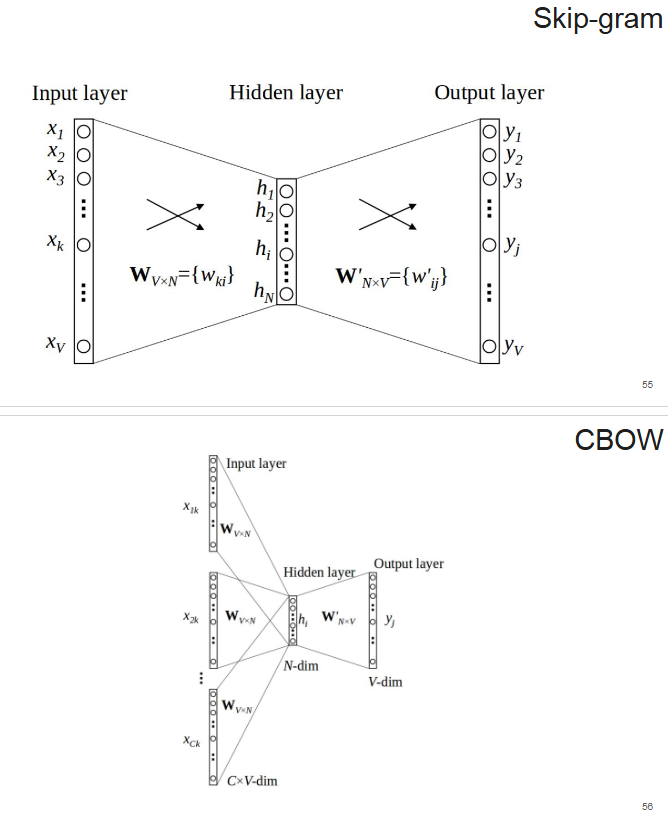
\includegraphics[width=0.9\textwidth]{figures/lecture01_cbow_vs_skipgram.png}
     \caption{Две основные архитектуры Word2Vec: CBOW и Skip-gram.}
\end{figure}
%
% ДОПОЛНИТЕЛЬНО, ЕСЛИ ЗАХОЧЕШЬ:
% Слайд 55: схема Skip-gram, lecture01_skipgram_architecture.png
% Слайд 56: схема CBOW, lecture01_cbow_architecture.png

\subsection{GloVe}

\textbf{GloVe} расшифровывается как \textbf{Global Vectors for Word Representation}.

Идея GloVe находится между двумя подходами:

\begin{itemize}
    \item count-based методами, которые используют статистику совместных встречаемостей;
    \item predictive методами, такими как Word2Vec.
\end{itemize}

Word2Vec обучается предсказывать близость слов через контекстные события.

GloVe обучается предсказывать статистики совместной встречаемости слов.

Пусть:

\[
X_{ij}
\]

--- количество раз, когда слово \(j\) встретилось в контексте слова \(i\).

GloVe минимизирует функцию потерь:

\[
J
=
\sum_{i,j=1}^{V}
f(X_{ij})
\left(
\bm{w}_i^\top \tilde{\bm{w}}_j
+
b_i
+
\tilde{b}_j
-
\log X_{ij}
\right)^2.
\]

Здесь:

\begin{itemize}
    \item \(\bm{w}_i\) --- обучаемый embedding слова \(i\);
    \item \(\tilde{\bm{w}}_j\) --- обучаемый embedding контекстного слова \(j\);
    \item \(b_i\), \(\tilde{b}_j\) --- обучаемые bias-параметры;
    \item \(X_{ij}\) --- co-occurrence count;
    \item \(f(X_{ij})\) --- весовая функция.
\end{itemize}

Смысл функции потерь:

\[
\bm{w}_i^\top \tilde{\bm{w}}_j
+
b_i
+
\tilde{b}_j
\]

должно приближать:

\[
\log X_{ij}.
\]

То есть скалярное произведение embeddings должно кодировать логарифм частоты совместной встречаемости.

Весовая функция \(f(X_{ij})\) нужна, чтобы:

\begin{itemize}
    \item уменьшать влияние слишком редких совместных встречаемостей;
    \item регуляризовать влияние слишком частых пар;
    \item сделать обучение устойчивее.
\end{itemize}

\subsection{Сравнение подходов к представлению текста}

\begin{table}[H]
\centering
\begin{tabular}{p{0.25\textwidth} p{0.35\textwidth} p{0.3\textwidth}}
\toprule
\textbf{Метод} & \textbf{Идея} & \textbf{Проблемы / особенности} \\
\midrule

One-hot &
Каждое слово --- отдельный sparse-вектор. &
Нет семантической близости, огромная размерность. \\

Bag-of-Words &
Документ --- вектор частот слов. &
Теряется порядок слов, sparse-векторы. \\

Bag-of-Ngrams &
Используются последовательности из \(n\) слов. &
Размерность быстро растёт. \\

TF-IDF &
Слова взвешиваются по важности для документа и редкости в корпусе. &
Хорошо для классических моделей, но не даёт плотной семантики. \\

PMI / pPMI &
Используются статистики совместной встречаемости слов. &
Можно получать семантическую близость, но матрицы большие. \\

Word2Vec &
Векторы обучаются через предсказание контекста. &
Эффективные dense embeddings, нужны оптимизации. \\

GloVe &
Векторы обучаются предсказывать co-occurrence statistics. &
Соединяет count-based и neural-подходы. \\

\bottomrule
\end{tabular}
\caption{Основные способы представления текста и слов.}
\end{table}

\subsection{Главные выводы}

\begin{itemize}
    \item Текст нельзя напрямую подать в классическую ML-модель: его нужно преобразовать в числовые признаки.
    \item Bag-of-Words --- простой baseline, но он теряет порядок слов и даёт sparse-векторы.
    \item TF-IDF улучшает BoW, понижая вес слишком общих слов и повышая вес редких информативных слов.
    \item One-hot encoding представляет слова как независимые категории и не кодирует семантическое сходство.
    \item Distributional semantics говорит: значение слова определяется его контекстом.
    \item Word embeddings --- плотные векторы слов, в которых похожие слова должны иметь близкие представления.
    \item Word2Vec обучает embeddings через задачу предсказания контекста.
    \item В Skip-gram центральное слово используется для предсказания контекста.
    \item В CBOW контекст используется для предсказания центрального слова.
    \item Negative Sampling ускоряет обучение Word2Vec, обновляя только малую часть весов.
    \item GloVe обучает embeddings так, чтобы их скалярные произведения приближали статистики совместной встречаемости.
\end{itemize}

\subsection{Что важно помнить к экзамену}

\begin{enumerate}
    \item Уметь объяснить общий pipeline text classification:
    \[
    \text{text} \rightarrow \text{features} \rightarrow \text{classifier} \rightarrow \text{label}.
    \]

    \item Понимать разницу между stemming и lemmatization.

    \item Знать проблемы Bag-of-Words:
    \begin{itemize}
        \item нет порядка слов;
        \item огромная размерность;
        \item sparse-векторы;
        \item разные формы слов считаются разными словами.
    \end{itemize}

    \item Уметь записать формулу TF-IDF:
    \[
    tfidf(t,d,D)
    =
    tf(t,d)
    \cdot
    \log
    \frac{N}
    {|\{d \in D : t \in d\}|}.
    \]

    \item Понимать, почему one-hot vectors не кодируют смысл.

    \item Уметь объяснить distributional hypothesis:
    слова с похожими контекстами имеют похожие значения.

    \item Знать формулу PMI:
    \[
    PMI(u,v)
    =
    \log
    \frac{p(u,v)}{p(u)p(v)}.
    \]

    \item Знать, что такое pPMI:
    \[
    pPMI(u,v) = \max(0, PMI(u,v)).
    \]

    \item Уметь объяснить Word2Vec, CBOW и Skip-gram.

    \item Понимать, зачем нужен Negative Sampling.

    \item Знать основную идею GloVe:
    embeddings обучаются предсказывать логарифмы co-occurrence counts.
\end{enumerate}
```









```latex
\section{Лекция 2. CNN for Texts and Embeddings for Different Languages}

\subsection{План лекции}

В этой лекции рассматриваются три основные темы:

\begin{itemize}
    \item повторение Word2Vec и embeddings;
    \item embeddings для разных языков и задача перевода без параллельных данных;
    \item применение сверточных нейронных сетей к текстам.
\end{itemize}

Основная идея лекции: векторы слов можно использовать не только внутри одного языка, но и для сопоставления разных языков, а CNN можно применять к тексту как к последовательности локальных фрагментов, похожих на \(n\)-граммы.

\subsection{Повторение Word2Vec}

Word2Vec обучает плотные векторные представления слов через задачу предсказания контекста.

В модели Skip-gram центральное слово используется для предсказания соседних слов. Если есть предложение

\[
\text{The quick brown fox jumps over the lazy dog},
\]

то для центрального слова \textit{brown} и окна размера 2 можно получить обучающие пары:

\[
(\text{brown}, \text{the}), \quad
(\text{brown}, \text{quick}), \quad
(\text{brown}, \text{fox}), \quad
(\text{brown}, \text{jumps}).
\]

Идея состоит в том, что слова с похожими контекстами получают похожие векторные представления.

\begin{figure}[H]
    \centering
    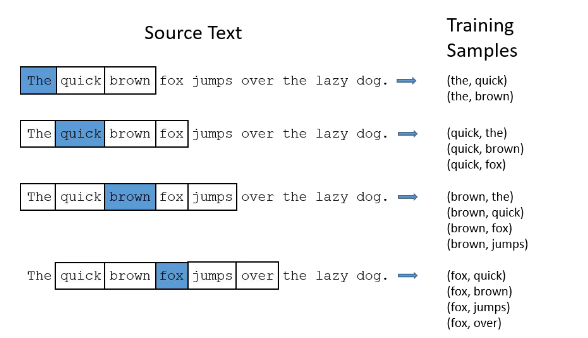
\includegraphics[width=0.9\textwidth]{figures/lecture02_word2vec_training_samples.png}
    \caption{Формирование обучающих пар в Skip-gram. Слайд 3.}
\end{figure}

Архитектурно Word2Vec можно представить как нейронную сеть:

\begin{itemize}
    \item вход --- one-hot вектор слова;
    \item скрытый слой --- плотное представление слова;
    \item выход --- распределение вероятностей по словам словаря.
\end{itemize}

Если размер словаря равен \(V\), а размерность embedding равна \(d\), то матрица входных весов имеет размер

\[
V \times d.
\]

Строки этой матрицы после обучения становятся векторами слов.

\begin{figure}[H]
    \centering
    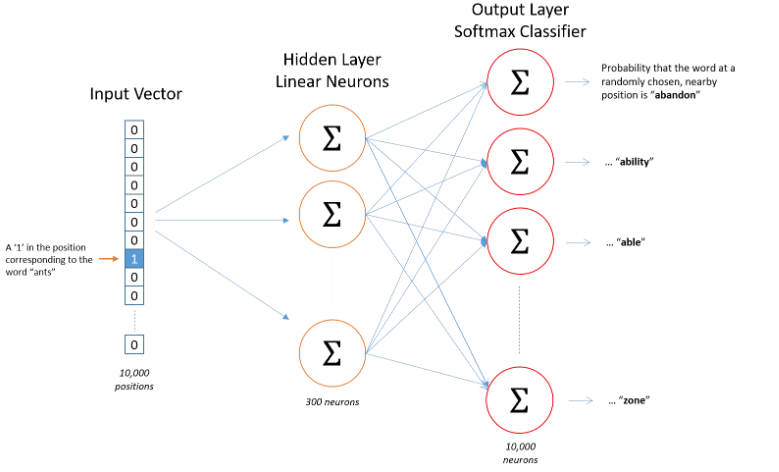
\includegraphics[width=0.85\textwidth]{figures/lecture02_word2vec_network.png}
    \caption{Word2Vec как нейронная сеть: one-hot вход, скрытый слой и softmax-выход. Слайд 4.}
\end{figure}

Матрицу весов скрытого слоя можно интерпретировать как lookup table:

\[
w_i \mapsto \bm{v}_{w_i}.
\]

То есть каждому слову сопоставляется строка матрицы --- его embedding.

\subsection{Embeddings для разных языков}

Оказывается, что embedding-пространства разных языков часто имеют похожую геометрическую структуру.

Например, в одном языке могут быть слова:

\[
\text{one}, \text{two}, \text{three}, \text{four}, \text{five},
\]

а в другом языке их переводы:

\[
\text{uno}, \text{dos}, \text{tres}, \text{cuatro}, \text{cinco}.
\]

Если обучить embeddings отдельно для каждого языка, относительное расположение таких слов может оказаться похожим. Аналогично могут сохраняться отношения между словами:

\[
\text{dog}, \text{cat}, \text{cow}, \text{horse}
\]

и их переводами в другом языке.

\begin{figure}[H]
    \centering
    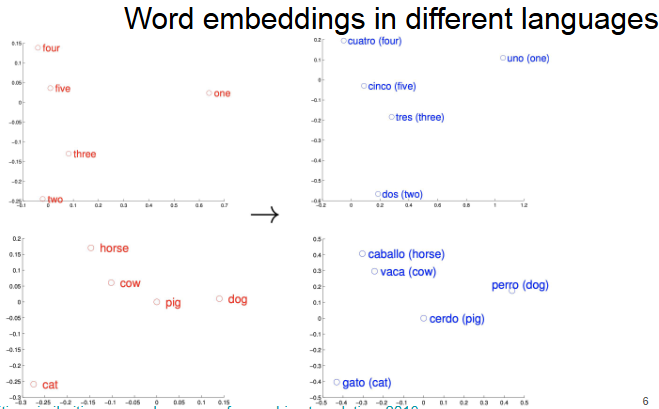
\includegraphics[width=0.85\textwidth]{figures/lecture02_crosslingual_embeddings_similarity.png}
    \caption{Похожая структура embedding-пространств для разных языков. Слайд 6.}
\end{figure}

Это позволяет решать задачу перевода слов через отображение одного embedding-пространства в другое.

\subsection{Линейное отображение между языками}

Пусть есть два языка:

\begin{itemize}
    \item source language --- исходный язык;
    \item target language --- целевой язык.
\end{itemize}

Для некоторого набора слов известны пары переводов:

\[
\{(x_i, y_i)\}_{i=1}^{n},
\]

где

\[
x_i \in \mathbb{R}^d
\]

--- embedding слова из исходного языка, а

\[
y_i \in \mathbb{R}^d
\]

--- embedding его перевода в целевом языке.

Например, можно взять

\[
n = 5000
\]

пар слов-переводов.

Идея: выучить линейное отображение

\[
W
\]

из source embedding space в target embedding space.

Если собрать векторы исходного языка в матрицу

\[
X \in \mathbb{R}^{d \times n},
\]

а векторы целевого языка в матрицу

\[
Y \in \mathbb{R}^{d \times n},
\]

то можно искать матрицу \(W\), минимизирующую расстояние между отображёнными исходными embeddings и целевыми embeddings:

\[
W^*
=
\arg\min_{W \in M_d(\mathbb{R})}
\|WX - Y\|_F.
\]

Здесь

\[
\|\cdot\|_F
\]

--- норма Фробениуса.

После обучения матрицы \(W\) перевод слова \(s\) можно искать так:

\[
t
=
\arg\max_t
\cos(Wx_s, y_t).
\]

То есть embedding исходного слова \(x_s\) сначала отображается в пространство целевого языка, а затем среди всех слов целевого языка выбирается ближайший вектор по cosine similarity.

\subsection{Ортогональное отображение}

На практике часто накладывают ограничение ортогональности на матрицу \(W\):

\[
W \in O_d(\mathbb{R}).
\]

Это означает:

\[
W^\top W = I.
\]

Ортогональное преобразование сохраняет длины и углы между векторами. Это полезно, потому что при переводе между языками мы хотим не произвольно деформировать пространство, а в основном повернуть или отразить его так, чтобы оно совпало с другим языком.

Задача принимает вид:

\[
W^*
=
\arg\min_{W \in O_d(\mathbb{R})}
\|WX - Y\|_F.
\]

Решение можно выразить через SVD:

\[
U \Sigma V^\top = SVD(YX^\top),
\]

\[
W^* = UV^\top.
\]

После этого перевод снова ищется по ближайшему вектору:

\[
t
=
\arg\max_t
\cos(Wx_s, y_t).
\]


\subsection{Unsupervised mapping между языками}

В презентации отмечается, что отображение между двумя языками может быть построено и полностью unsupervised способом, например с использованием GAN.

Идея в общих чертах:

\begin{itemize}
    \item есть два набора embeddings \(X\) и \(Y\);
    \item нет известных пар переводов;
    \item модель пытается найти такое отображение \(W\), чтобы распределение \(WX\) стало похоже на распределение \(Y\);
    \item после грубого выравнивания можно уточнять соответствия между словами.
\end{itemize}

Это важная идея для cross-lingual NLP: можно сопоставлять языки даже без параллельного корпуса и без большого словаря переводов.

\begin{figure}[H]
    \centering
    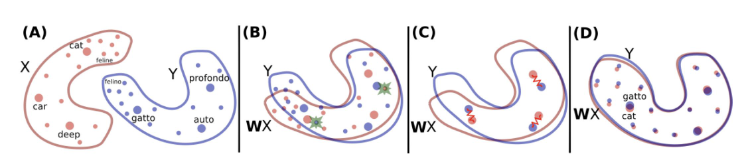
\includegraphics[width=0.9\textwidth]{figures/lecture02_unsupervised_mapping_gan.png}
    \caption{Интуиция unsupervised mapping между embedding-пространствами двух языков. Слайд 9.}
\end{figure}

\subsection{Cosine similarity}

Для сравнения векторов часто используют cosine similarity:

\[
\cos(\theta)
=
\frac{\bm{A} \cdot \bm{B}}
{\|\bm{A}\| \|\bm{B}\|}.
\]

В координатной форме:

\[
\cos(\theta)
=
\frac{
\sum_{i=1}^{n} A_i B_i
}
{
\sqrt{\sum_{i=1}^{n} A_i^2}
\sqrt{\sum_{i=1}^{n} B_i^2}
}.
\]

Cosine similarity измеряет не абсолютное расстояние между концами векторов, а угол между ними.

Это полезно для текстовых векторов, потому что длина вектора может сильно зависеть от частоты слова или длины документа. Например, в count-based подходах длинные документы могут иметь большие нормы просто потому, что в них больше слов.

Для word embeddings cosine similarity также часто оказывается удобной, потому что направление embedding-вектора обычно важнее его нормы.

\subsection{Норма embedding-вектора и частота слова}

В презентации показано, что норма embedding-вектора может зависеть от частоты слова в корпусе.

Более частые слова могут получать embeddings с большей евклидовой нормой. Поэтому если сравнивать векторы обычным скалярным произведением, частотность слова может сильно влиять на результат.

Именно поэтому часто используют cosine similarity:

\[
\cos(\bm{u}, \bm{v})
=
\frac{\bm{u}^\top \bm{v}}
{\|\bm{u}\|\|\bm{v}\|}.
\]

Нормировка убирает влияние длины векторов и оставляет в основном направление.

\subsection{Как получить embedding для текста}

Word embeddings дают представления отдельных слов. Но во многих задачах нужен embedding всего текста:

\[
[w_1, w_2, \dots, w_n]
\mapsto
\bm{h}_{text}.
\]

Один простой способ --- усреднить embeddings слов:

\[
\bm{h}_{text}
=
\frac{1}{n}
\sum_{i=1}^{n}
\bm{v}_{w_i}.
\]

Но такой подход теряет порядок слов.

Другой способ --- использовать модели последовательностей, например RNN, LSTM или GRU.

\subsection{Повторение RNN}

\textbf{Recurrent Neural Network, RNN} обрабатывает последовательность слева направо. На каждом шаге она получает текущий вход \(x_t\) и предыдущее скрытое состояние \(h_{t-1}\):

\[
h_t = f(W_x x_t + W_h h_{t-1} + b).
\]

Для vanilla RNN часто используется:

\[
h_t = \tanh(W_x x_t + W_h h_{t-1} + b).
\]

Идея: скрытое состояние \(h_t\) должно содержать информацию о префиксе последовательности:

\[
x_1, x_2, \dots, x_t.
\]

Тогда финальное состояние \(h_n\) можно использовать как embedding всей последовательности.



Проблема RNN: финальный вектор может слишком сильно зависеть от последних слов и хуже хранить информацию о локальных фразах в середине текста.

Кроме того, обычные RNN сталкиваются с проблемой vanishing gradient. Поэтому на практике часто используют:

\begin{itemize}
    \item LSTM;
    \item GRU;
    \item skip connections;
    \item gradient clipping.
\end{itemize}

\subsection{Переход от RNN к CNN}

RNN естественно обрабатывает текст как последовательность. Но у неё есть недостаток: чтобы получить вектор для фразы, модель учитывает префиксный контекст.

Например, в фразе

\[
\text{the country of my birth}
\]

RNN будет постепенно накапливать информацию:

\[
\text{the}
\rightarrow
\text{the country}
\rightarrow
\text{the country of}
\rightarrow
\text{the country of my}
\rightarrow
\text{the country of my birth}.
\]

Но если нам нужны локальные фразы, например

\[
\text{country of}, \quad
\text{my birth}, \quad
\text{country of my birth},
\]

RNN не всегда даёт удобный независимый вектор для каждой такой фразы.

Идея CNN для текста: вычислять признаки для всех локальных фрагментов текста.


\subsection{\texorpdfstring{\(n\)-граммы}{n-граммы} и CNN}

В прошлой лекции рассматривались \(n\)-граммы. Например, для предложения

\[
\text{The brown dog plays with a little cat}
\]

биграммы:

\[
\text{The brown}, \quad
\text{brown dog}, \quad
\text{dog plays}, \quad
\text{plays with}, \quad
\text{with a}, \quad
\text{a little}, \quad
\text{little cat}.
\]

CNN для текста можно понимать как обобщение идеи \(n\)-грамм.

Фильтр размера \(h\) смотрит на окно из \(h\) соседних слов:

\[
x_{i:i+h-1}.
\]

Например:

\begin{itemize}
    \item фильтр размера \(1\) похож на unigram-признак;
    \item фильтр размера \(2\) похож на bigram-признак;
    \item фильтр размера \(3\) похож на trigram-признак.
\end{itemize}

Отличие от обычных \(n\)-грамм: CNN не просто считает частоты конкретных фраз, а обучает фильтры, которые могут находить полезные паттерны в embedding-пространстве.

\subsection{Свёртка по тексту}

Пусть текст представлен матрицей embeddings:

\[
X \in \mathbb{R}^{n \times d},
\]

где:

\begin{itemize}
    \item \(n\) --- длина текста;
    \item \(d\) --- размерность embedding;
    \item строка \(X_i\) --- embedding \(i\)-го слова.
\end{itemize}

Фильтр размера \(h\) применяется к окну:

\[
X_{i:i+h-1}.
\]

На каждом окне вычисляется признак:

\[
c_i
=
f(W^\top X_{i:i+h-1} + b).
\]

Здесь:

\begin{itemize}
    \item \(W\) --- параметры фильтра;
    \item \(b\) --- bias;
    \item \(f\) --- нелинейная функция активации;
    \item \(c_i\) --- значение feature map в позиции \(i\).
\end{itemize}

Если фильтр применяется ко всем возможным позициям, получается feature map:

\[
\bm{c}
=
[c_1, c_2, \dots, c_{n-h+1}]
\in
\mathbb{R}^{n-h+1}.
\]

\begin{figure}[H]
    \centering
    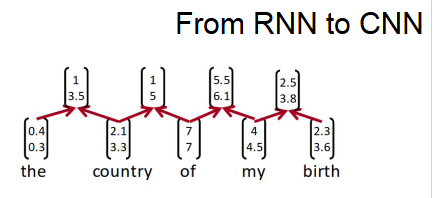
\includegraphics[width=0.85\textwidth]{figures/lecture02_bigram_convolution.png}
    \caption{Операция над каждой парой соседних слов может интерпретироваться как свёртка по word vectors. Слайд 23.}
\end{figure}

\subsection{One-layer CNN для текста}

Один слой CNN для текста обычно состоит из:

\begin{enumerate}
    \item embedding layer;
    \item convolutional layer;
    \item pooling layer;
    \item fully connected layer;
    \item output layer.
\end{enumerate}

Свёртка строит feature map:

\[
\bm{c}
=
[c_1, c_2, \dots, c_{n-h+1}].
\]

Затем применяется pooling. Самый распространённый вариант для классификации текста --- max-over-time pooling:

\[
\hat{c}
=
\max \bm{c}.
\]

Это означает, что из всей feature map берётся максимальное значение.

Интерпретация:

\begin{itemize}
    \item фильтр ищет некоторый паттерн в тексте;
    \item max pooling отвечает на вопрос: встретился ли этот паттерн где-нибудь в тексте;
    \item позиция паттерна становится неважной.
\end{itemize}

После pooling длина текста уже не имеет значения. Поэтому можно использовать тексты разной длины и фильтры разных размеров:

\[
h = 1, 2, 3, 4, \dots
\]

То есть модель может одновременно искать unigram-, bigram-, trigram- и более длинные паттерны.



\subsection{CNN architecture from Kim 2014}

Классическая архитектура CNN для sentence classification была предложена Kim в 2014 году.

Общая схема:

\begin{itemize}
    \item предложение представляется как матрица word embeddings;
    \item применяются несколько convolutional filters разных ширин;
    \item для каждого фильтра строится feature map;
    \item по каждой feature map применяется max-over-time pooling;
    \item полученные признаки объединяются;
    \item затем идут dropout, fully connected layer и softmax.
\end{itemize}

Если использовать фильтры разных размеров, модель может находить признаки на уровне разных \(n\)-грамм.

Например:

\[
h = 2
\]

ищет bigram-like паттерны,

\[
h = 3
\]

ищет trigram-like паттерны,

\[
h = 4
\]

ищет более длинные фразы.

\begin{figure}[H]
    \centering
    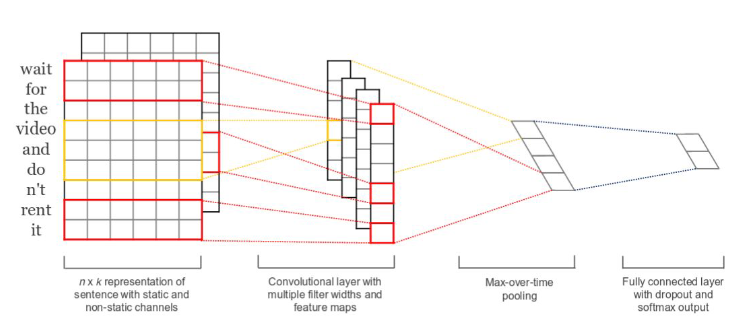
\includegraphics[width=0.9\textwidth]{figures/lecture02_kim2014_cnn.png}
    \caption{CNN для классификации предложений из статьи Kim, 2014. Слайд 26.}
\end{figure}

\subsection{Static и non-static embeddings}

В CNN для текстов embeddings могут использоваться по-разному.

\textbf{Static embeddings}:

\begin{itemize}
    \item берутся заранее обученные embeddings;
    \item во время обучения модели они не обновляются;
    \item полезно, если мало обучающих данных.
\end{itemize}

\textbf{Non-static embeddings}:

\begin{itemize}
    \item embeddings инициализируются предобученными векторами;
    \item затем дообучаются вместе с основной моделью;
    \item могут лучше адаптироваться к конкретной задаче.
\end{itemize}

\textbf{Multichannel embeddings}:

\begin{itemize}
    \item используется несколько каналов embeddings;
    \item например, один канал static, другой non-static;
    \item аналогия с каналами изображения в CNN.
\end{itemize}

\subsection{Narrow и wide convolution}

В CNN для текста можно различать narrow и wide convolution.

\textbf{Narrow convolution} применяется только там, где фильтр полностью помещается внутрь последовательности. Для длины текста \(n\) и ширины фильтра \(h\) длина feature map равна:

\[
n - h + 1.
\]

\textbf{Wide convolution} использует zero-padding, то есть добавляет нулевые векторы по краям последовательности. Это позволяет фильтру применяться также к позициям около границ текста.

Padding полезен, потому что:

\begin{itemize}
    \item крайние слова тоже получают полноценную обработку;
    \item можно управлять размером выходной feature map;
    \item можно строить более глубокие CNN без слишком быстрого уменьшения длины последовательности.
\end{itemize}

Также можно использовать stride:

\[
s > 1.
\]

Stride означает, что фильтр сдвигается не на одну позицию, а на несколько.

\subsection{Применения CNN в NLP}

CNN использовались в разных NLP-задачах:

\begin{itemize}
    \item классификация предложений;
    \item sentiment analysis;
    \item question classification;
    \item neural machine translation;
    \item построение sentence embeddings.
\end{itemize}

В ранних моделях neural machine translation CNN могли использоваться как encoder, а RNN --- как decoder.

То есть CNN сжимает исходное предложение в представление, а RNN затем генерирует перевод.


\subsection{Сравнение подходов}

В презентации приведена таблица результатов разных моделей на NLP-бенчмарках. Основная идея таблицы: CNN-based модели оказались конкурентоспособными с другими подходами для классификации текста.

Сравнивались варианты:

\begin{itemize}
    \item CNN-rand;
    \item CNN-static;
    \item CNN-non-static;
    \item CNN-multichannel;
    \item RAE;
    \item MV-RNN;
    \item RNTN;
    \item DCNN;
    \item Paragraph-Vec;
    \item SVM и другие baseline-модели.
\end{itemize}

Важный практический вывод: даже относительно простая CNN-архитектура с предобученными embeddings может давать сильные результаты в задачах классификации текста.

\subsection{Outro and tips}

Главные практические замечания из лекции:

\begin{itemize}
    \item Vanishing gradient встречается не только в RNN, но и в глубоких нейронных сетях вообще.
    \item Для борьбы с vanishing gradient используют memory mechanisms, skip connections и другие архитектурные приёмы.
    \item LSTM и GRU хорошо подходят для последовательностей.
    \item GRU обычно быстрее, а LSTM может лучше ловить сложные зависимости.
    \item Полезно использовать gradient clipping.
    \item CNN для текстов похожи на обучаемый \(n\)-gram trick.
    \item CNN эффективны, когда можно параллельно выполнять много вычислений.
    \item RNN и CNN можно комбинировать.
\end{itemize}

\subsection{Attention как следующая тема}

В конце лекции упоминается attention.

В машинном переводе attention позволяет модели явно сопоставлять слова исходного предложения со словами целевого предложения.

Визуально attention часто изображают как матрицу alignment:

\[
A_{ij},
\]

где \(A_{ij}\) показывает, насколько сильно \(i\)-е слово перевода связано с \(j\)-м словом исходного предложения.

В примере из Bahdanau et al. attention показывает почти диагональную структуру соответствий между английским и французским предложениями, но также позволяет учитывать перестановки слов.

\begin{figure}[H]
    \centering
    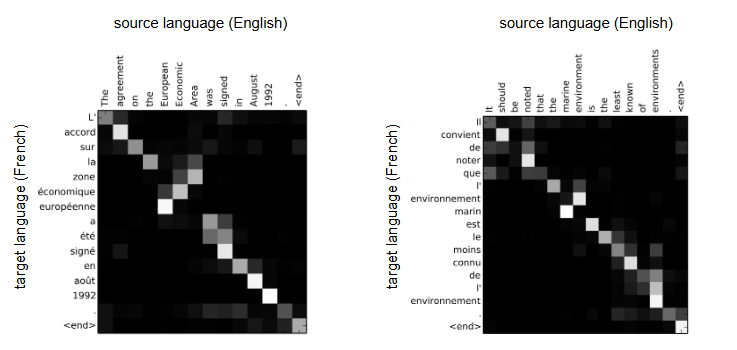
\includegraphics[width=0.85\textwidth]{figures/lecture02_attention_alignment.png}
    \caption{Attention alignment в neural machine translation. Слайд 31.}
\end{figure}

Эта тема важна, потому что attention затем станет основой архитектуры Transformer.

\subsection{Проблема Word2Vec}

В финале презентации подчёркивается ограничение Word2Vec:

\[
\text{Word2Vec embeddings capture only local context.}
\]

То есть Word2Vec обучается на локальных окнах вокруг слова. Поэтому он хорошо отражает локальную совместную встречаемость, но не всегда достаточно хорошо учитывает:

\begin{itemize}
    \item дальние зависимости;
    \item структуру всего предложения;
    \item разные значения одного слова в разных контекстах;
    \item глобальный смысл текста.
\end{itemize}

Это мотивирует переход к более сложным моделям контекстуальных представлений: RNN, CNN, attention и Transformer.

\subsection{Главные выводы}

\begin{itemize}
    \item Word2Vec строит embeddings слов через задачу предсказания контекста.
    \item Матрица весов скрытого слоя Word2Vec фактически является таблицей embeddings.
    \item Embedding-пространства разных языков часто имеют похожую структуру.
    \item Перевод слов можно делать через линейное отображение между embedding-пространствами.
    \item Ортогональное отображение сохраняет углы и длины, поэтому хорошо подходит для cross-lingual mapping.
    \item Cosine similarity удобна для сравнения embeddings, потому что фокусируется на направлении векторов, а не на их длине.
    \item RNN строит представление текста последовательно, но может плохо выделять локальные фразы.
    \item CNN для текста можно понимать как обучаемые \(n\)-gram detectors.
    \item Свёрточный фильтр проходит по окнам слов и строит feature map.
    \item Max-over-time pooling делает длину текста несущественной и фиксирует наличие паттерна в тексте.
    \item CNN с предобученными embeddings является сильным baseline для классификации текста.
    \item Attention решает задачу явного сопоставления частей входной и выходной последовательности.
\end{itemize}

\subsection{Что важно помнить к экзамену}

\begin{enumerate}
    \item Уметь объяснить, почему embedding-пространства разных языков можно сопоставлять.

    \item Знать задачу линейного mapping:
    \[
    W^*
    =
    \arg\min_W
    \|WX - Y\|_F.
    \]

    \item Знать ортогональный вариант:
    \[
    W^*
    =
    \arg\min_{W \in O_d(\mathbb{R})}
    \|WX - Y\|_F.
    \]

    \item Помнить решение через SVD:
    \[
    U \Sigma V^\top = SVD(YX^\top),
    \quad
    W^* = UV^\top.
    \]

    \item Уметь записать cosine similarity:
    \[
    \cos(\theta)
    =
    \frac{\bm{A} \cdot \bm{B}}
    {\|\bm{A}\|\|\bm{B}\|}.
    \]

    \item Понимать, почему cosine similarity лучше обычного dot product для embeddings.

    \item Уметь объяснить, как CNN применяется к тексту:
    \[
    c_i
    =
    f(W^\top X_{i:i+h-1} + b).
    \]

    \item Понимать, что фильтр размера \(h\) похож на обучаемый \(h\)-gram detector.

    \item Знать max-over-time pooling:
    \[
    \hat{c} = \max \bm{c}.
    \]

    \item Уметь сравнить RNN и CNN для текста:
    \begin{itemize}
        \item RNN хорошо моделирует последовательность;
        \item CNN хорошо ловит локальные паттерны;
        \item CNN легче параллелить.
    \end{itemize}

    \item Помнить ограничение Word2Vec:
    он в основном учитывает локальный контекст.
\end{enumerate}
```



```latex
\section{Лекция 3. Machine Translation and Attention Mechanism}

\subsection{План лекции}

В этой лекции рассматриваются:

\begin{itemize}
    \item исторический обзор машинного перевода;
    \item statistical machine translation;
    \item word alignment;
    \item phrase-based machine translation;
    \item neural machine translation;
    \item архитектура seq2seq;
    \item greedy decoding и beam search;
    \item оценка качества машинного перевода;
    \item attention mechanism.
\end{itemize}

Главная идея лекции: машинный перевод прошёл путь от rule-based и statistical machine translation к neural machine translation. В нейронном машинном переводе важнейшей архитектурой стала encoder-decoder схема, а attention был введён как способ устранить bottleneck фиксированного вектора, в который encoder должен был сжать всё исходное предложение.

\subsection{Исторический обзор машинного перевода}

Машинный перевод --- одна из старейших задач NLP. Уже в 1950-е годы появились первые эксперименты по автоматическому переводу.

Один из первых известных экспериментов --- Georgetown experiment, проведённый 7 января 1954 года. В нём выполнялся автоматический перевод с русского на английский:

\begin{itemize}
    \item переводилось 60 предложений;
    \item использовался словарь примерно из 250 словарных статей;
    \item использовалось 6 грамматических правил;
    \item вычисления выполнялись на IBM 701.
\end{itemize}

В СССР в 1954 году также проводились эксперименты по машинному переводу на БЭСМ. Эти ранние системы были rule-based: они опирались на словари и вручную заданные правила.

Дальше развитие машинного перевода можно грубо разделить на несколько этапов:

\begin{itemize}
    \item rule-based machine translation;
    \item expert systems;
    \item statistical machine translation;
    \item neural machine translation.
\end{itemize}

\subsection{Обучающие данные для машинного перевода}

Для обучения систем машинного перевода обычно используются \textbf{parallel corpora}.

\textbf{Parallel corpus} --- корпус, состоящий из пар:

\[
\langle \text{source}, \text{translation} \rangle.
\]

Обычно это пары предложений:

\[
(x, y),
\]

где:

\begin{itemize}
    \item \(x\) --- предложение на исходном языке;
    \item \(y\) --- его перевод на целевой язык.
\end{itemize}

Иногда параллельные данные могут быть выровнены на уровне абзацев или документов, но чаще используется sentence-level alignment.

Параллельные корпуса могут быть:

\begin{itemize}
    \item вручную подготовлены переводчиками;
    \item собраны из веба;
    \item сгенерированы синтетически.
\end{itemize}

\subsection{Statistical Machine Translation}

\textbf{Statistical Machine Translation, SMT} --- подход к машинному переводу, доминировавший примерно в 1990--2010 годы.

Пусть есть предложение \(x\) на исходном языке. Нужно найти наиболее вероятный перевод \(y\) на целевом языке:

\[
\hat{y}
=
\arg\max_y P(y \mid x).
\]

С помощью правила Байеса:

\[
P(y \mid x)
=
\frac{P(x \mid y)P(y)}{P(x)}.
\]

Так как \(x\) фиксировано, знаменатель \(P(x)\) не влияет на выбор максимума:

\[
\hat{y}
=
\arg\max_y P(x \mid y)P(y).
\]

Здесь появляются две основные компоненты SMT:

\begin{itemize}
    \item \textbf{translation model} \(P(x \mid y)\) --- оценивает, насколько хорошо предложение \(y\) переводится в \(x\);
    \item \textbf{language model} \(P(y)\) --- оценивает, насколько предложение \(y\) является естественным предложением на целевом языке.
\end{itemize}

Иными словами:

\[
\text{translation model} \quad \text{отвечает за adequacy},
\]

\[
\text{language model} \quad \text{отвечает за fluency}.
\]

\textbf{Adequacy} означает, что перевод сохраняет смысл исходного предложения.  
\textbf{Fluency} означает, что перевод звучит естественно на целевом языке.

% Слайд 7. SMT: разложение вероятности перевода по Байесу на translation model и language model.
\begin{figure}[H]
    \centering
    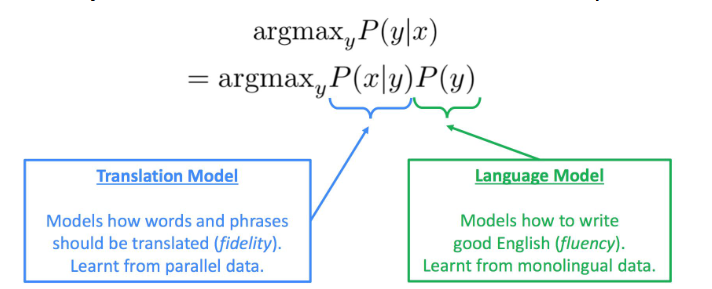
\includegraphics[width=0.9\textwidth]{figures/lecture03_smt_bayes.png}
    \caption{Statistical Machine Translation: разложение задачи перевода на translation model и language model.}
\end{figure}

\subsection{Word Alignment}

Чтобы обучить translation model из параллельного корпуса, нужно понять, какие слова исходного предложения соответствуют каким словам перевода.

\textbf{Alignment} --- соответствие между словами исходного предложения и словами целевого предложения.

Пусть:

\[
x = (x_1, x_2, \dots, x_m)
\]

--- предложение на исходном языке, а

\[
y = (y_1, y_2, \dots, y_n)
\]

--- предложение на целевом языке.

Alignment задаёт связи между словами \(x_i\) и \(y_j\).

В простейшем случае слово соответствует одному слову:

\[
x_i \leftrightarrow y_j.
\]

Но в реальных языках всё сложнее.

\subsubsection{Many-to-one alignment}

Несколько слов одного языка могут соответствовать одному слову другого языка.

Например, английское словосочетание может переводиться одним словом во французском или наоборот.

Это называется:

\[
\text{many-to-one alignment}.
\]

\subsubsection{One-to-many alignment}

Одно слово одного языка может соответствовать нескольким словам другого языка.

В презентации это связывается с понятием \textbf{fertility}.

\textbf{Fertility} слова --- количество слов в переводе, которым соответствует данное слово.

Если одно слово порождает много слов в переводе, оно называется highly fertile.

\subsubsection{Many-to-many alignment}

На практике часто возникает соответствие не слово-к-слову, а фраза-к-фразе.

Например:

\[
\text{do not have any money}
\]

может переводиться как цельное выражение, и отдельные слова могут не иметь независимых прямых соответствий.

Такое соответствие называется:

\[
\text{many-to-many alignment}.
\]

% Слайд 12. Пример many-to-many alignment и phrase alignment.
\begin{figure}[H]
    \centering
    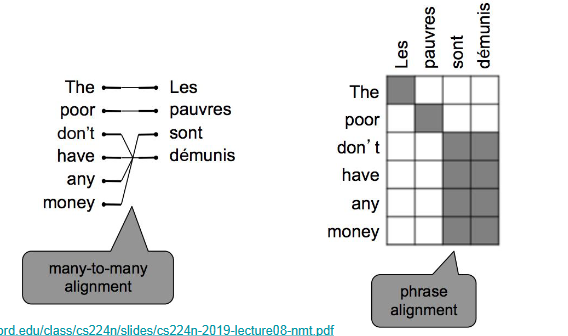
\includegraphics[width=0.85\textwidth]{figures/lecture03_word_alignment_many_to_many.png}
    \caption{Пример many-to-many alignment: соответствие между фразами, а не отдельными словами.}
\end{figure}

\subsection{Почему полный перебор переводов невозможен}

В SMT нужно найти:

\[
\hat{y}
=
\arg\max_y P(x \mid y)P(y).
\]

Но множество возможных переводов \(y\) огромно. Нельзя перебрать все возможные предложения на целевом языке и посчитать вероятность каждого.

Поэтому используются эвристические алгоритмы поиска, которые:

\begin{itemize}
    \item строят перевод постепенно;
    \item хранят только наиболее вероятные гипотезы;
    \item отбрасывают низковероятные варианты.
\end{itemize}

Эта идея позже появится и в neural machine translation в виде beam search.

\subsection{Phrase-Based Machine Translation}

\textbf{Phrase-Based Machine Translation, PBMT} --- развитие SMT, где перевод выполняется не отдельными словами, а фразами.

Здесь \textbf{phrase} не обязательно означает грамматическую фразу. Это может быть просто последовательность из нескольких слов, то есть \(n\)-грамма.

PBMT использует:

\begin{itemize}
    \item \textbf{phrase table};
    \item \textbf{\(n\)-gram language model}.
\end{itemize}

\subsubsection{Phrase table}

Phrase table хранит возможные переводы фраз и их вероятности или стоимости.

Например, для source phrase:

\[
\text{I saw a cat}
\]

могут быть варианты перевода:

\[
\text{Я видел кошку},
\]

\[
\text{Я увидел кошку},
\]

\[
\text{Я видел кошечку}.
\]

Каждому варианту сопоставляется score, например:

\[
-\log P.
\]

Чем меньше значение \(-\log P\), тем выше вероятность.

\subsubsection{\texorpdfstring{\(n\)-gram}{n-gram} language model}

Language model оценивает вероятность следующего слова по предыдущему контексту:

\[
P(w_t \mid w_{t-n+1}, \dots, w_{t-1}).
\]

Она помогает выбрать перевод, который звучит естественно на целевом языке.

Например, если модель видела много предложений вида:

\[
\text{I saw a cat},
\]

\[
\text{I saw a dog},
\]

то она понимает, что после \textit{I saw a} вероятно существительное.

\subsubsection{Недостатки PBMT}

PBMT-системы имели много отдельно проектируемых компонентов:

\begin{itemize}
    \item phrase table;
    \item language model;
    \item distortion model;
    \item reordering model;
    \item feature weights;
    \item decoding algorithm.
\end{itemize}

Это приводило к проблемам:

\begin{itemize}
    \item много feature engineering;
    \item нужно вручную проектировать признаки под языковые явления;
    \item нужно поддерживать большие таблицы фраз;
    \item много человеческих усилий;
    \item для каждой языковой пары работу приходилось повторять.
\end{itemize}

% Слайд 16. PBMT: phrase table и поиск перевода как композиция фраз.
\begin{figure}[H]
    \centering
    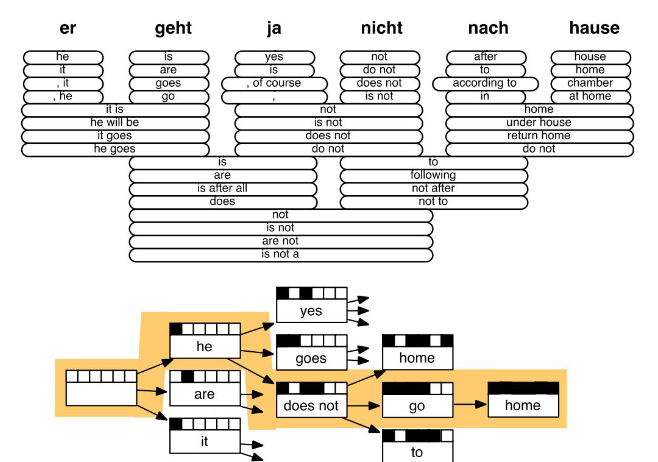
\includegraphics[width=0.85\textwidth]{figures/lecture03_pbmt_search.png}
    \caption{Phrase-Based Machine Translation: перевод строится из фразовых соответствий и оценивается языковой моделью.}
\end{figure}

\subsection{Neural Machine Translation}

\textbf{Neural Machine Translation, NMT} --- подход, в котором машинный перевод выполняется одной нейронной сетью.

Вместо множества вручную спроектированных компонентов используется end-to-end обучение:

\[
x \mapsto y.
\]

NMT напрямую моделирует:

\[
P(y \mid x),
\]

где:

\begin{itemize}
    \item \(x\) --- source sentence;
    \item \(y\) --- target sentence.
\end{itemize}

Классическая архитектура NMT называется:

\[
\text{sequence-to-sequence}
\]

или сокращённо:

\[
\text{seq2seq}.
\]

\subsection{Seq2Seq}

\textbf{Seq2Seq} состоит из двух основных частей:

\begin{itemize}
    \item encoder;
    \item decoder.
\end{itemize}

\subsubsection{Encoder}

Encoder читает исходное предложение:

\[
x = (x_1, x_2, \dots, x_m)
\]

и преобразует его в скрытое представление.

Если encoder является RNN, то на каждом шаге:

\[
h_i = f(h_{i-1}, x_i).
\]

Финальное состояние encoder-а:

\[
h_m
\]

считается вектором, который кодирует всё исходное предложение.

\subsubsection{Decoder}

Decoder генерирует перевод по одному токену.

Он начинает со специального токена:

\[
\langle SOS \rangle,
\]

а затем на каждом шаге предсказывает следующий токен:

\[
y_t.
\]

Генерация продолжается до специального токена:

\[
\langle EOS \rangle.
\]

Формально:

\[
P(y \mid x)
=
\prod_{t=1}^{T}
P(y_t \mid y_1, \dots, y_{t-1}, x).
\]

Или короче:

\[
P(y \mid x)
=
\prod_{t=1}^{T}
P(y_t \mid y_{<t}, x).
\]

% Слайд 25. Полная схема seq2seq decoding: encoder передаёт состояние decoder-у, decoder генерирует перевод по токенам.
\begin{figure}[H]
    \centering
    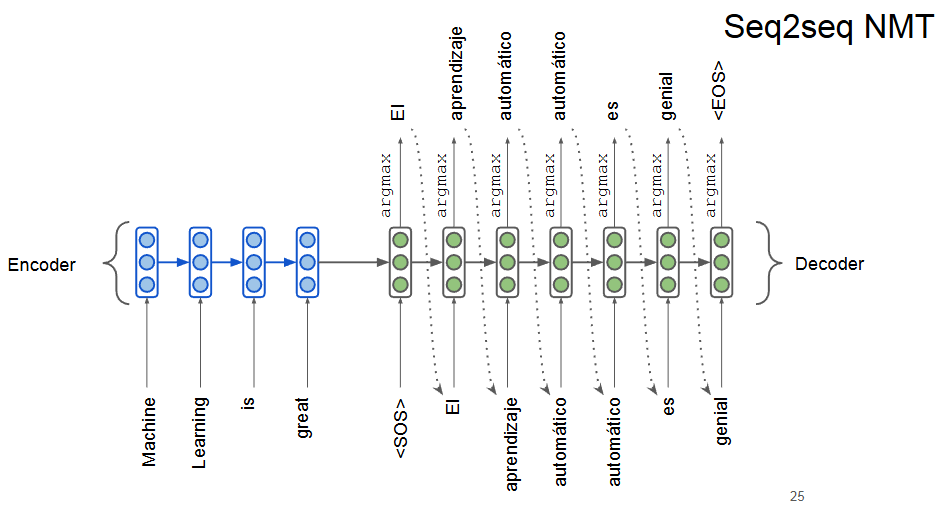
\includegraphics[width=0.9\textwidth]{figures/lecture03_seq2seq_decoding.png}
    \caption{Seq2seq NMT: encoder кодирует исходное предложение, decoder генерирует перевод токен за токеном.}
\end{figure}

\subsection{Обучение Seq2Seq}

Seq2seq обучается end-to-end на параллельном корпусе.

Для каждой пары:

\[
(x, y)
\]

модель максимизирует вероятность правильного перевода:

\[
P(y \mid x).
\]

Обычно минимизируется negative log-likelihood:

\[
\mathcal{L}
=
-\log P(y \mid x).
\]

С учётом разложения по токенам:

\[
\mathcal{L}
=
-
\sum_{t=1}^{T}
\log P(y_t \mid y_{<t}, x).
\]

Интуитивно модель штрафуется каждый раз, когда она даёт низкую вероятность правильному следующему токену перевода.

Во время обучения часто используется teacher forcing: на вход decoder-а на следующем шаге подаётся правильный предыдущий токен, а не обязательно токен, предсказанный самой моделью.

\subsection{Greedy Decoding}

После обучения нужно сгенерировать перевод.

Самый простой способ --- \textbf{greedy decoding}.

На каждом шаге decoder выбирает наиболее вероятный токен:

\[
\hat{y}_t
=
\arg\max_{w}
P(w \mid \hat{y}_{<t}, x).
\]

Потом выбранный токен подаётся на следующий шаг.

Проблема greedy decoding:

\begin{itemize}
    \item локально лучший токен не обязательно ведёт к глобально лучшему предложению;
    \item если модель ошиблась на раннем шаге, эта ошибка становится частью входа на следующих шагах;
    \item ошибки могут накапливаться.
\end{itemize}

То есть greedy decoding делает жадный выбор без рассмотрения альтернатив.

\subsection{Exhaustive Search}

Теоретически хотелось бы найти перевод:

\[
\hat{y}
=
\arg\max_y P(y \mid x).
\]

Но:

\[
P(y \mid x)
=
P(y_1 \mid x)
\prod_{t=2}^{T}
P(y_t \mid y_1, \dots, y_{t-1}, x).
\]

Если размер словаря равен \(V\), а длина перевода равна \(T\), то число возможных последовательностей порядка:

\[
V^T.
\]

Это экспоненциальная сложность, поэтому полный перебор невозможен.

\subsection{Beam Search}

\textbf{Beam Search} --- компромисс между greedy decoding и полным перебором.

Идея:

\begin{itemize}
    \item на каждом шаге хранить не одну лучшую гипотезу, а \(k\) лучших частичных переводов;
    \item \(k\) называется beam size;
    \item на практике часто используют \(k \approx 5\)--\(10\);
    \item на каждом шаге все текущие гипотезы расширяются возможными следующими словами;
    \item затем снова оставляются только top-\(k\) гипотез.
\end{itemize}

Гипотеза:

\[
(y_1, \dots, y_t)
\]

имеет score, равный логарифму вероятности:

\[
score(y_1,\dots,y_t)
=
\log P_{LM}(y_1,\dots,y_t \mid x).
\]

С учётом авторегрессионного разложения:

\[
score(y_1,\dots,y_t)
=
\sum_{i=1}^{t}
\log P_{LM}(y_i \mid y_1,\dots,y_{i-1}, x).
\]

Beam search ищет high-scoring hypotheses, но не гарантирует нахождение глобально оптимального перевода.

% Слайд 31. Пример beam search decoding при beam size k = 2.
\begin{figure}[H]
    \centering
    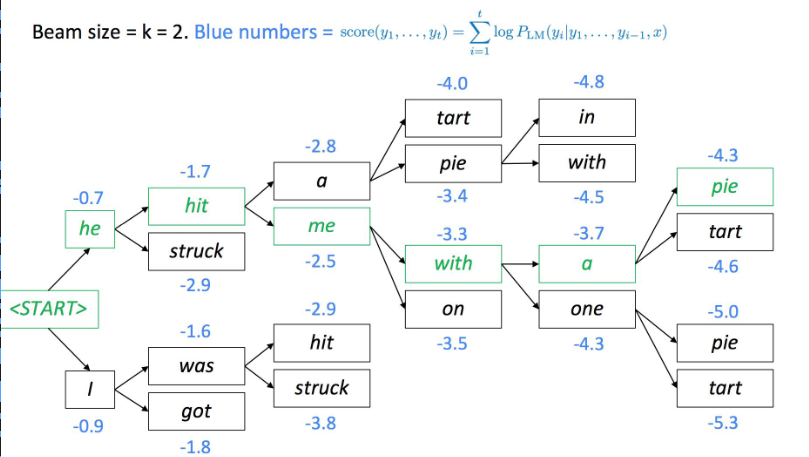
\includegraphics[width=0.9\textwidth]{figures/lecture03_beam_search_example.png}
    \caption{Пример beam search decoding: на каждом шаге сохраняются top-\(k\) частичных гипотез.}
\end{figure}

\subsection{Критерий остановки Beam Search}

В greedy decoding обычно генерация продолжается до тех пор, пока модель не выдаст:

\[
\langle EOS \rangle.
\]

В beam search разные гипотезы могут завершиться на разных шагах.

Если гипотеза породила:

\[
\langle EOS \rangle,
\]

то она считается завершённой. Её можно отложить в список completed hypotheses, а beam search продолжает развивать остальные гипотезы.

Обычно beam search продолжают до одного из условий:

\begin{itemize}
    \item достигнут заранее заданный максимальный timestep \(T\);
    \item накоплено достаточно завершённых гипотез;
    \item все гипотезы завершились.
\end{itemize}

\subsection{Length Normalization}

У beam search есть проблема: длинные гипотезы обычно имеют меньший score.

Причина: score является суммой логарифмов вероятностей:

\[
score(y_1,\dots,y_t)
=
\sum_{i=1}^{t}
\log P_{LM}(y_i \mid y_1,\dots,y_{i-1}, x).
\]

Так как вероятности меньше или равны 1, их логарифмы обычно неположительны:

\[
\log P \leq 0.
\]

Чем больше токенов, тем больше отрицательных слагаемых. Поэтому длинные переводы штрафуются просто за длину.

Простая коррекция --- нормировать score на длину:

\[
score_{norm}(y_1,\dots,y_t)
=
\frac{1}{t}
\sum_{i=1}^{t}
\log P_{LM}(y_i \mid y_1,\dots,y_{i-1}, x).
\]

Это позволяет сравнивать гипотезы разной длины более честно.

\subsection{Оценка качества машинного перевода}

Для оценки качества машинного перевода используются автоматические и человеческие метрики.

\subsection{BLEU}

\textbf{BLEU} расшифровывается как:

\[
\text{Bilingual Evaluation Understudy}.
\]

BLEU сравнивает машинный перевод с человеческим reference translation.

Метрика основана на двух идеях:

\begin{itemize}
    \item \(n\)-gram precision;
    \item brevity penalty.
\end{itemize}

\subsubsection{\texorpdfstring{\(n\)-gram precision}{n-gram precision}}

\(n\)-gram precision измеряет, какая доля \(n\)-грамм машинного перевода встречается в reference translation.

Например, для unigram precision:

\[
precision_1
=
\frac{
\text{число совпавших unigram}
}{
\text{число unigram в машинном переводе}
}.
\]

Аналогично можно считать:

\[
precision_2, \quad precision_3, \quad precision_4.
\]

\subsubsection{Brevity penalty}

Если система выдаёт слишком короткий перевод, она может получить искусственно высокую precision.

Например, если reference:

\[
\text{the cat sits on the mat},
\]

а система выдала только:

\[
\text{the cat},
\]

то precision может быть высокой, но перевод неполный.

Поэтому BLEU использует brevity penalty.

В упрощённой форме из лекции:

\[
brevity\ penalty
=
\min
\left(
1,
\frac{output\ length}{reference\ length}
\right).
\]

\subsubsection{Формула BLEU}

Для \(n\)-грамм до порядка \(n\):

\[
BLEU
=
brevity\ penalty
\cdot
\left(
\prod_{i=1}^{n}
precision_i
\right)^{1/n}
\cdot
100\%.
\]

Смысл:

\begin{itemize}
    \item высокая BLEU означает сильное \(n\)-граммное совпадение с reference translation;
    \item brevity penalty штрафует слишком короткие переводы;
    \item геометрическое среднее делает метрику чувствительной к плохим precision на больших \(n\)-граммах.
\end{itemize}

\subsection{Недостатки BLEU}

BLEU несовершенна.

Главная проблема: одно и то же предложение можно корректно перевести разными способами.

Если хороший перевод использует другие слова или другой порядок слов, он может получить низкий BLEU из-за малого \(n\)-gram overlap с reference.

То есть BLEU хорошо подходит для быстрой автоматической оценки на корпусном уровне, но плохо отражает качество отдельных переводов.

\subsection{Другие метрики качества MT}

Кроме BLEU, используются:

\begin{itemize}
    \item \textbf{ROUGE} --- Recall-Oriented Understudy for Gisting Evaluation;
    \item \textbf{METEOR} --- Metric for Evaluation of Translation with Explicit ORdering;
    \item human evaluation;
    \item ML-based quality estimation.
\end{itemize}

METEOR может использовать синонимы из WordNet, поэтому она менее жёстко зависит от буквального совпадения слов.

\subsection{Human Evaluation}

Человеческая оценка качества перевода может быть устроена по-разному.

\subsubsection{Side-by-side human evaluation}

Человеку показывают исходное предложение и несколько переводов.

Задача:

\[
\text{выбрать лучший перевод}.
\]

Например:

\begin{itemize}
    \item System 1: плохой или неестественный перевод;
    \item System 2: более корректный перевод.
\end{itemize}

\subsubsection{Direct Assessment}

В Direct Assessment человеку показывают один перевод и просят оценить его по шкале, например от 1 до 5.

Человеческая оценка обычно качественнее автоматических метрик, но она дорогая.

\subsection{ML-based quality estimation}

Так как human evaluation дорогая, появляются модели, обученные приближать человеческую оценку.

Примеры:

\begin{itemize}
    \item \textbf{BLEURT} --- модель Google, BERT fine-tuned на Direct Assessment ratings;
    \item \textbf{XCOMET} --- модель Unbabel, XLM fine-tuned на DA и MQM ratings;
    \item \textbf{LLM-based estimators} --- использование больших языковых моделей для оценки качества перевода.
\end{itemize}

\subsection{Преимущества NMT}

Преимущества neural machine translation:

\begin{itemize}
    \item лучшее качество перевода;
    \item более fluent output;
    \item лучшее использование контекста;
    \item лучшее использование похожести фраз;
    \item одна нейронная сеть оптимизируется end-to-end;
    \item нет необходимости вручную оптимизировать множество отдельных компонентов;
    \item меньше feature engineering;
    \item один и тот же общий подход можно применять к разным языковым парам.
\end{itemize}

\subsection{Недостатки NMT}

Недостатки neural machine translation:

\begin{itemize}
    \item модель менее интерпретируема;
    \item её труднее отлаживать;
    \item поведение модели сложнее контролировать;
    \item трудно явно задать правила или guidelines для перевода;
    \item возможны safety concerns.
\end{itemize}

Нейронные модели могут давать странные переводы на необычных входах, опечатках, повторяющихся символах или фразах вне распределения обучающих данных.

\subsection{Решён ли машинный перевод?}

Машинный перевод нельзя считать полностью решённой задачей.

Остаются проблемы:

\begin{itemize}
    \item использование большого контекста;
    \item low-resource language pairs;
    \item отсутствие больших параллельных корпусов для многих языков;
    \item сленг;
    \item узкие домены;
    \item устойчивость к ошибкам и опечаткам;
    \item контроль качества и безопасности перевода.
\end{itemize}

\subsection{Bottleneck в Seq2Seq}

В классическом seq2seq вся информация об исходном предложении должна быть сжата в один вектор --- финальное hidden state encoder-а.

\[
h_m
\]

используется как начальное состояние decoder-а.

Проблема: если исходное предложение длинное или сложное, один вектор может стать узким местом.

Это называется:

\[
\text{bottleneck}.
\]

Decoder должен генерировать весь перевод, опираясь на одно фиксированное представление исходного предложения. Поэтому модель может терять детали, особенно для длинных предложений.

% Слайд 48. Bottleneck в seq2seq: одно финальное состояние encoder-а должно кодировать всё предложение.
\begin{figure}[H]
    \centering
    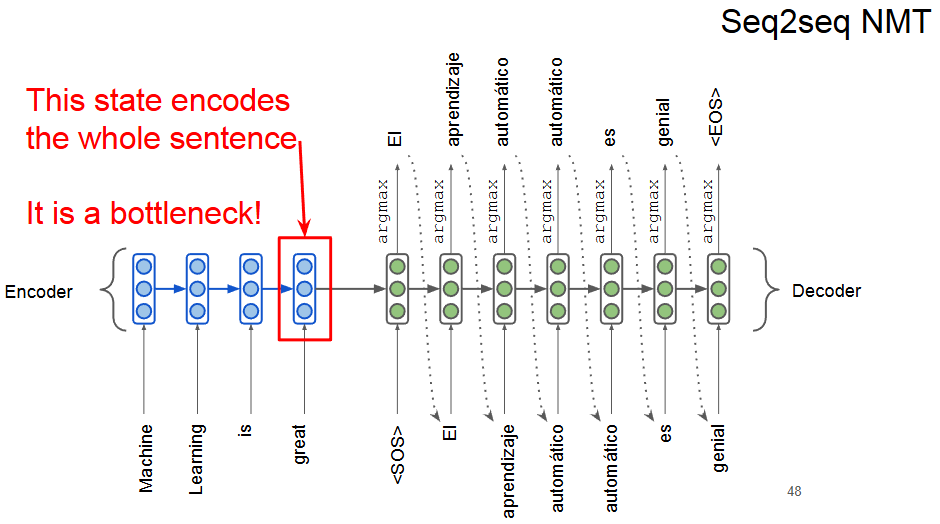
\includegraphics[width=0.9\textwidth]{figures/lecture03_seq2seq_bottleneck.png}
    \caption{Bottleneck классического seq2seq: всё исходное предложение кодируется одним состоянием encoder-а.}
\end{figure}

\subsection{Attention: основная идея}

\textbf{Attention} решает проблему bottleneck.

Основная идея:

\begin{quote}
На каждом шаге decoder-а использовать прямое соединение с encoder-ом, чтобы фокусироваться на конкретной части исходной последовательности.
\end{quote}

То есть decoder больше не обязан пользоваться только одним финальным вектором encoder-а. Вместо этого на каждом шаге генерации он может смотреть на все hidden states encoder-а:

\[
h_1, h_2, \dots, h_m.
\]

Для каждого шага decoder-а attention вычисляет:

\begin{itemize}
    \item насколько важен каждый encoder state;
    \item distribution внимания по source tokens;
    \item weighted sum encoder states;
    \item context vector для текущего шага decoder-а.
\end{itemize}

\subsection{Seq2Seq with Attention}

Пусть encoder породил hidden states:

\[
h_1, h_2, \dots, h_m.
\]

Пусть decoder на шаге \(t\) имеет состояние:

\[
s_t.
\]

Attention вычисляет score для каждой позиции исходного предложения:

\[
e_{t,i}
=
score(s_t, h_i).
\]

Score показывает, насколько encoder state \(h_i\) важен для decoder-а на шаге \(t\).

Затем scores нормируются softmax-ом:

\[
\alpha_{t,i}
=
\frac{
\exp(e_{t,i})
}{
\sum_{j=1}^{m}
\exp(e_{t,j})
}.
\]

Коэффициенты:

\[
\alpha_{t,1}, \dots, \alpha_{t,m}
\]

образуют attention distribution:

\[
\sum_{i=1}^{m} \alpha_{t,i} = 1.
\]

После этого строится attention output, или context vector:

\[
c_t
=
\sum_{i=1}^{m}
\alpha_{t,i} h_i.
\]

То есть context vector --- это взвешенная сумма всех encoder states.

Затем \(c_t\) объединяется с состоянием decoder-а \(s_t\) и используется для предсказания следующего токена:

\[
P(y_t \mid y_{<t}, x).
\]

% Слайд 52. Attention: scores -> softmax distribution -> weighted sum of encoder states.
\begin{figure}[H]
    \centering
    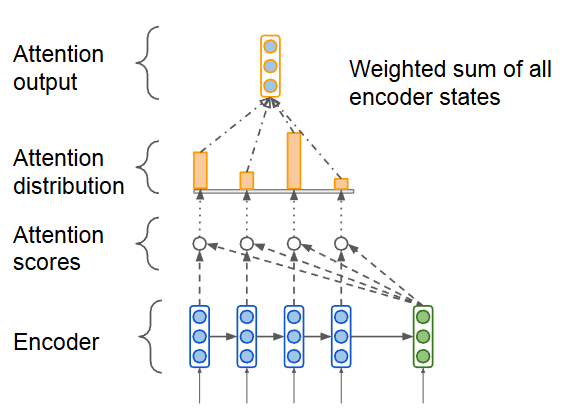
\includegraphics[width=0.85\textwidth]{figures/lecture03_attention_weighted_sum.png}
    \caption{Seq2seq with attention: scores преобразуются softmax-ом в attention distribution, затем строится weighted sum encoder states.}
\end{figure}

\subsection{Attention в формулах}

Обозначим:

\[
h_i
\]

--- hidden state encoder-а для \(i\)-го source token.

\[
s_t
\]

--- hidden state decoder-а на шаге \(t\).

\subsubsection{Dot-product attention}

Самый простой вариант score:

\[
e_{t,i}
=
s_t^\top h_i.
\]

Чем больше скалярное произведение, тем больше похожи состояния decoder-а и encoder-а, тем больше внимания получает позиция \(i\).

Attention distribution:

\[
\alpha_{t}
=
\operatorname{softmax}(e_t).
\]

Компонентно:

\[
\alpha_{t,i}
=
\frac{
\exp(s_t^\top h_i)
}{
\sum_{j=1}^{m}
\exp(s_t^\top h_j)
}.
\]

Context vector:

\[
c_t
=
\sum_{i=1}^{m}
\alpha_{t,i}h_i.
\]

\subsubsection{Multiplicative attention}

В multiplicative attention добавляется обучаемая матрица \(W\):

\[
e_{t,i}
=
s_t^\top W h_i.
\]

Здесь \(W\) позволяет модели обучить более гибкую меру совместимости между decoder state и encoder state.

\subsubsection{Additive attention}

В additive attention score вычисляется через маленькую нейронную сеть:

\[
e_{t,i}
=
v^\top
\tanh(W_1 h_i + W_2 s_t).
\]

Здесь:

\begin{itemize}
    \item \(W_1\), \(W_2\) --- обучаемые матрицы;
    \item \(v\) --- обучаемый вектор;
    \item \(\tanh\) добавляет нелинейность.
\end{itemize}

Additive attention часто связывают с работой Bahdanau et al. ``Neural Machine Translation by Jointly Learning to Align and Translate'', 2014.

\subsection{Интерпретируемость Attention}

Attention даёт частичную интерпретируемость.

На каждом шаге decoder-а можно посмотреть attention distribution:

\[
\alpha_{t,1}, \dots, \alpha_{t,m}.
\]

Она показывает, на какие слова source sentence модель обращала внимание при генерации текущего target token.

Это похоже на word alignment:

\[
\text{source tokens}
\leftrightarrow
\text{target tokens}.
\]

Поэтому говорят, что attention даёт word alignment ``for free''.

Важно понимать: attention weights не всегда являются идеальным объяснением работы модели, но для машинного перевода они часто дают полезную визуализацию соответствий между словами.

\subsection{Почему Attention важен}

Attention стал ключевым механизмом, потому что:

\begin{itemize}
    \item снимает bottleneck фиксированного вектора encoder-а;
    \item позволяет decoder-у обращаться к разным частям source sentence на разных шагах;
    \item улучшает перевод длинных предложений;
    \item даёт полезные alignment-визуализации;
    \item стал основой дальнейшего развития NLP-архитектур.
\end{itemize}

Позже идея attention приведёт к Transformer, где attention станет главным механизмом обработки последовательностей.

\subsection{Сравнение SMT, PBMT и NMT}

\begin{table}[H]
\centering
\begin{tabular}{p{0.25\textwidth} p{0.35\textwidth} p{0.3\textwidth}}
\toprule
\textbf{Подход} & \textbf{Идея} & \textbf{Проблемы} \\
\midrule

SMT &
Использует вероятностную модель \(P(x \mid y)P(y)\). &
Много независимых компонентов, сложный feature engineering. \\

PBMT &
Переводит фразами, использует phrase table и \(n\)-gram LM. &
Нужно хранить и поддерживать phrase tables, плохо масштабируется на новые языковые пары. \\

NMT &
Одна нейронная сеть напрямую моделирует \(P(y \mid x)\). &
Менее интерпретируема, сложнее контролировать, требует большие данные. \\

Seq2seq without attention &
Encoder сжимает всё предложение в один вектор, decoder генерирует перевод. &
Bottleneck для длинных и сложных предложений. \\

Seq2seq with attention &
Decoder на каждом шаге смотрит на разные encoder states. &
Лучше работает с длинным контекстом, но всё ещё требует аккуратного обучения и декодирования. \\

\bottomrule
\end{tabular}
\caption{Сравнение подходов к машинному переводу.}
\end{table}

\subsection{Главные выводы}

\begin{itemize}
    \item Statistical Machine Translation ищет перевод через:
    \[
    \arg\max_y P(x \mid y)P(y).
    \]

    \item В SMT есть две главные части:
    \begin{itemize}
        \item translation model;
        \item language model.
    \end{itemize}

    \item Word alignment описывает соответствия между словами исходного и целевого предложений.

    \item Alignment бывает:
    \begin{itemize}
        \item one-to-one;
        \item many-to-one;
        \item one-to-many;
        \item many-to-many.
    \end{itemize}

    \item PBMT переводит не отдельными словами, а фразами.

    \item Neural Machine Translation моделирует \(P(y \mid x)\) одной нейронной сетью.

    \item Seq2seq состоит из encoder-а и decoder-а.

    \item Decoder генерирует перевод авторегрессионно:
    \[
    P(y \mid x)
    =
    \prod_{t=1}^{T}
    P(y_t \mid y_{<t}, x).
    \]

    \item Greedy decoding выбирает самый вероятный токен на каждом шаге, но может ошибаться глобально.

    \item Beam search хранит top-\(k\) гипотез на каждом шаге и является практическим компромиссом.

    \item BLEU оценивает перевод через \(n\)-gram precision и brevity penalty.

    \item Классический seq2seq имеет bottleneck: всё исходное предложение сжимается в один вектор.

    \item Attention позволяет decoder-у на каждом шаге обращаться ко всем hidden states encoder-а.

    \item Attention context vector:
    \[
    c_t
    =
    \sum_{i=1}^{m}
    \alpha_{t,i}h_i.
    \]

    \item Attention улучшает перевод длинных предложений и даёт интерпретируемое alignment-подобное поведение.
\end{itemize}

\subsection{Что важно помнить к экзамену}

\begin{enumerate}
    \item Формулу SMT через Байеса:
    \[
    \hat{y}
    =
    \arg\max_y P(y \mid x)
    =
    \arg\max_y P(x \mid y)P(y).
    \]

    \item Что такое translation model и language model.

    \item Что такое word alignment и какие бывают типы alignment.

    \item Что PBMT использует phrase tables и \(n\)-gram language model.

    \item Почему SMT/PBMT требуют много feature engineering.

    \item Что NMT напрямую моделирует:
    \[
    P(y \mid x).
    \]

    \item Разложение вероятности перевода в seq2seq:
    \[
    P(y \mid x)
    =
    \prod_{t=1}^{T}
    P(y_t \mid y_{<t}, x).
    \]

    \item Loss для обучения:
    \[
    \mathcal{L}
    =
    -
    \sum_{t=1}^{T}
    \log P(y_t \mid y_{<t}, x).
    \]

    \item Чем greedy decoding отличается от beam search.

    \item Score гипотезы в beam search:
    \[
    score(y_1,\dots,y_t)
    =
    \sum_{i=1}^{t}
    \log P_{LM}(y_i \mid y_1,\dots,y_{i-1}, x).
    \]

    \item Зачем нужна length normalization.

    \item Формулу BLEU:
    \[
    BLEU
    =
    brevity\ penalty
    \cdot
    \left(
    \prod_{i=1}^{n}
    precision_i
    \right)^{1/n}
    \cdot
    100\%.
    \]

    \item Почему BLEU несовершенна.

    \item Что bottleneck в seq2seq --- это необходимость сжать всё source sentence в один вектор.

    \item Основную идею attention:
    decoder на каждом шаге фокусируется на разных hidden states encoder-а.

    \item Формулы attention:
    \[
    e_{t,i} = score(s_t, h_i),
    \]
    \[
    \alpha_{t,i}
    =
    \frac{\exp(e_{t,i})}
    {\sum_{j=1}^{m}\exp(e_{t,j})},
    \]
    \[
    c_t
    =
    \sum_{i=1}^{m}
    \alpha_{t,i}h_i.
    \]

    \item Три варианта attention score:
    \begin{itemize}
        \item dot-product:
        \[
        e_{t,i}=s_t^\top h_i;
        \]

        \item multiplicative:
        \[
        e_{t,i}=s_t^\top W h_i;
        \]

        \item additive:
        \[
        e_{t,i}
        =
        v^\top
        \tanh(W_1h_i + W_2s_t).
        \]
    \end{itemize}
\end{enumerate}
```


```latex
\section{Лекция 4. Self-Attention and Transformer}

\subsection{План лекции}

В этой лекции рассматриваются:

\begin{itemize}
    \item краткое повторение CNN для текстов;
    \item повторение attention в seq2seq;
    \item архитектура Transformer;
    \item self-attention;
    \item multi-head attention;
    \item positional encoding;
    \item layer normalization;
    \item decoder side и masked self-attention.
\end{itemize}

Главная идея лекции: Transformer заменяет рекуррентность и свёртки механизмом self-attention. Благодаря этому модель может напрямую связывать любые позиции последовательности, хорошо параллелится и эффективно работает с длинными зависимостями.

\subsection{Повторение: CNN для текстов}

CNN для текстов можно понимать как обучаемый аналог \(n\)-граммных признаков.

Пусть текст представлен матрицей embeddings:

\[
X \in \mathbb{R}^{n \times d},
\]

где:

\begin{itemize}
    \item \(n\) --- длина последовательности;
    \item \(d\) --- размерность embedding;
    \item строка \(X_i\) --- embedding \(i\)-го токена.
\end{itemize}

Свёрточный фильтр размера \(h\) применяется к окну:

\[
X_{i:i+h-1}.
\]

Значение признака в позиции \(i\):

\[
c_i = f(W^\top X_{i:i+h-1} + b).
\]

После применения фильтра ко всем позициям получается feature map:

\[
\bm{c}
=
[c_1, c_2, \dots, c_{n-h+1}].
\]

Для классификации текста часто используется max-over-time pooling:

\[
\hat{c} = \max_i c_i.
\]

Смысл: фильтр ищет некоторый паттерн в тексте, а max pooling проверяет, встретился ли этот паттерн где-нибудь.

CNN для текста хорошо ловит локальные паттерны, но для моделирования дальних зависимостей нужны либо глубокие сети, либо другие механизмы.

\subsection{Повторение: attention в seq2seq}

В seq2seq без attention encoder сжимает всё исходное предложение в один финальный вектор. Это создаёт bottleneck: decoder должен генерировать перевод, опираясь на одно фиксированное представление всего входа.

Attention решает эту проблему: на каждом шаге decoder может обращаться ко всем hidden states encoder-а.

Пусть encoder породил состояния:

\[
h_1, h_2, \dots, h_N,
\quad
h_i \in \mathbb{R}^h.
\]

Пусть на шаге \(t\) decoder имеет состояние:

\[
s_t \in \mathbb{R}^h.
\]

Для каждого encoder state вычисляется attention score:

\[
e_{t,i} = s_t^\top h_i.
\]

В векторной форме:

\[
e^t =
[s_t^\top h_1, \dots, s_t^\top h_N]
\in \mathbb{R}^N.
\]

Затем применяется softmax:

\[
\alpha^t = \operatorname{softmax}(e^t).
\]

Вектор \(\alpha^t\) является распределением внимания:

\[
\sum_{i=1}^{N} \alpha_i^t = 1.
\]

Attention output:

\[
a_t =
\sum_{i=1}^{N}
\alpha_i^t h_i.
\]

Затем \(a_t\) конкатенируется с decoder state:

\[
[a_t; s_t],
\]

и используется для предсказания следующего токена.

\subsection{Варианты attention score}

В лекции повторяются три основных варианта attention.

\subsubsection{Dot-product attention}

\[
e_i = s^\top h_i.
\]

Это самый простой вариант: совместимость decoder state и encoder state считается скалярным произведением.

\subsubsection{Multiplicative attention}

\[
e_i = s^\top W h_i.
\]

Здесь \(W\) --- обучаемая матрица. Она позволяет модели выучить более гибкую меру совместимости.

\subsubsection{Additive attention}

\[
e_i =
v^\top \tanh(W_1 h_i + W_2 s).
\]

Здесь:

\begin{itemize}
    \item \(W_1\), \(W_2\) --- обучаемые матрицы;
    \item \(v\) --- обучаемый вектор;
    \item \(\tanh\) добавляет нелинейность.
\end{itemize}

\subsection{Преимущества attention}

Attention даёт два важных преимущества:

\begin{itemize}
    \item \textbf{Free word alignment}: можно посмотреть, на какие слова source sentence модель обращает внимание при генерации каждого target token.
    \item \textbf{Better results on long sequences}: модель лучше работает с длинными последовательностями, потому что decoder не ограничен одним финальным состоянием encoder-а.
\end{itemize}

% Слайд 21. Attention advantages: сравнение качества на длинных последовательностях и пример alignment matrix.
\begin{figure}[H]
    \centering
    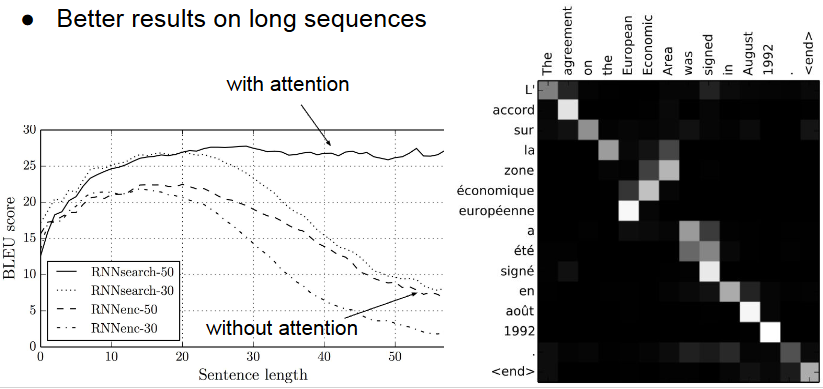
\includegraphics[width=0.85\textwidth]{figures/lecture04_attention_advantages.png}
    \caption{Преимущества attention: лучшее качество на длинных последовательностях и интерпретируемое выравнивание слов.}
\end{figure}

\subsection{Transformer: общая идея}

\textbf{Transformer} --- архитектура, предложенная в статье \textit{Attention is All You Need}.

Ключевая идея:

\[
\text{никаких RNN и CNN, только attention}.
\]

Transformer был предложен для машинного перевода и показал сильные результаты на WMT 2014 English-to-German translation task. В лекции указано значение:

\[
28.4 \text{ BLEU}.
\]

Главные свойства Transformer:

\begin{itemize}
    \item использует self-attention;
    \item не использует рекуррентные связи;
    \item хорошо параллелится;
    \item имеет короткий путь между любыми двумя позициями последовательности;
    \item стал базовой архитектурой для современных NLP-моделей.
\end{itemize}

\subsection{Encoder-decoder структура Transformer}

Transformer в классическом виде состоит из двух частей:

\begin{itemize}
    \item encoder stack;
    \item decoder stack.
\end{itemize}

Encoder читает входную последовательность и строит контекстуальные представления токенов.

Decoder генерирует выходную последовательность авторегрессионно, используя:

\begin{itemize}
    \item уже сгенерированные target tokens;
    \item выходы encoder-а;
    \item masked self-attention;
    \item encoder-decoder attention.
\end{itemize}

% Слайд 25. Transformer как стек encoder-блоков и decoder-блоков.
\begin{figure}[H]
    \centering
    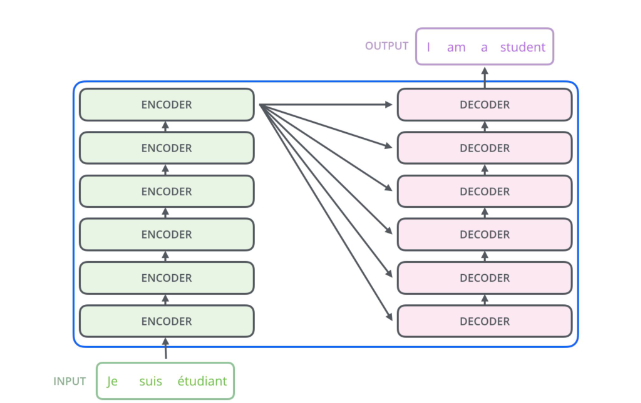
\includegraphics[width=0.85\textwidth]{figures/lecture04_transformer_stack.png}
    \caption{Transformer состоит из стека encoder-блоков и decoder-блоков.}
\end{figure}

\subsection{Encoder block}

Один encoder block состоит из двух основных подслоёв:

\begin{enumerate}
    \item self-attention layer;
    \item feed-forward neural network.
\end{enumerate}

Схематически:

\[
X
\longrightarrow
\text{Self-Attention}
\longrightarrow
Z
\longrightarrow
\text{Feed Forward}
\longrightarrow
R.
\]

Self-attention позволяет каждому токену учитывать другие токены входной последовательности.

Feed-forward network применяется к каждой позиции независимо, но с общими параметрами для всех позиций.

% Слайд 26. Encoder side: self-attention + feed-forward network.
\begin{figure}[H]
    \centering
    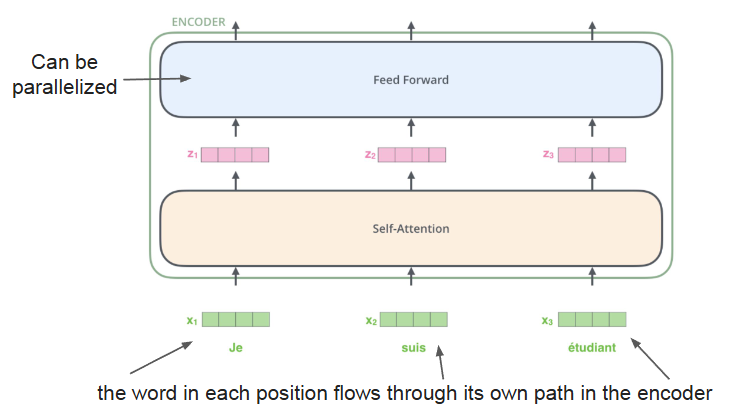
\includegraphics[width=0.8\textwidth]{figures/lecture04_encoder_block.png}
    \caption{Один encoder block: self-attention layer и feed-forward layer.}
\end{figure}

Важное отличие от RNN: позиции последовательности не обрабатываются строго последовательно. Поэтому вычисления внутри слоя можно эффективно параллелить.

\subsection{Self-Attention: интуиция}

Self-attention нужен, чтобы при обработке каждого токена учитывать другие релевантные токены той же последовательности.

Пример из лекции:

\[
\text{The animal didn't cross the street because it was too tired}.
\]

Вопрос:

\[
\text{к чему относится } \textit{it}?
\]

Правильная связь:

\[
\textit{it} \rightarrow \textit{animal}.
\]

Self-attention должен позволить представлению слова \textit{it} включить информацию о слове \textit{animal}.

То есть новое представление токена становится контекстуальным: оно зависит не только от самого токена, но и от других слов предложения.

% Слайд 35. Self-attention связывает слово "it" с релевантными словами в предложении.
\begin{figure}[H]
    \centering
    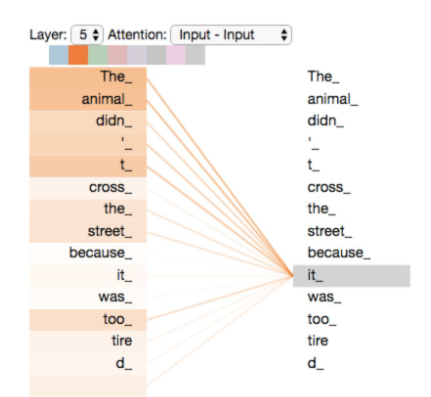
\includegraphics[width=0.75\textwidth]{figures/lecture04_self_attention_high_level.png}
    \caption{Self-attention позволяет токену учитывать другие релевантные токены той же последовательности.}
\end{figure}

\subsection{Query, Key, Value}

В self-attention из каждого входного embedding строятся три вектора:

\[
q_i, \quad k_i, \quad v_i.
\]

Они называются:

\begin{itemize}
    \item \textbf{Query};
    \item \textbf{Key};
    \item \textbf{Value}.
\end{itemize}

Пусть входной embedding токена:

\[
x_i \in \mathbb{R}^{d_{model}}.
\]

Тогда:

\[
q_i = W^Q x_i,
\]

\[
k_i = W^K x_i,
\]

\[
v_i = W^V x_i.
\]

Здесь \(W^Q\), \(W^K\), \(W^V\) --- обучаемые матрицы.

Интуиция:

\begin{itemize}
    \item \textbf{Query} --- что текущий токен ищет;
    \item \textbf{Key} --- что токен предлагает для сопоставления;
    \item \textbf{Value} --- какая информация будет передана, если на этот токен обратят внимание.
\end{itemize}

\subsection{Self-Attention для одного токена}

Рассмотрим токен в позиции \(i\).

Сначала считаем score между query текущего токена и key каждого токена:

\[
score(i,j) = q_i^\top k_j.
\]

Это показывает, насколько токен \(i\) должен обратить внимание на токен \(j\).

Затем scores масштабируются:

\[
\frac{q_i^\top k_j}{\sqrt{d_k}}.
\]

Деление на \(\sqrt{d_k}\) нужно для численной стабильности. Если размерность \(d_k\) большая, скалярные произведения могут иметь большую дисперсию, softmax становится слишком резким, и градиенты ухудшаются.

Затем применяется softmax:

\[
\alpha_{ij}
=
\frac{
\exp \left( \frac{q_i^\top k_j}{\sqrt{d_k}} \right)
}{
\sum_{\ell=1}^{n}
\exp \left( \frac{q_i^\top k_\ell}{\sqrt{d_k}} \right)
}.
\]

После этого выход self-attention для позиции \(i\):

\[
z_i
=
\sum_{j=1}^{n}
\alpha_{ij} v_j.
\]

То есть новый вектор токена --- это взвешенная сумма value-векторов всех токенов.

% Слайд 41. Self-attention: scores делятся на sqrt(d_k), затем применяется softmax.
\begin{figure}[H]
    \centering
    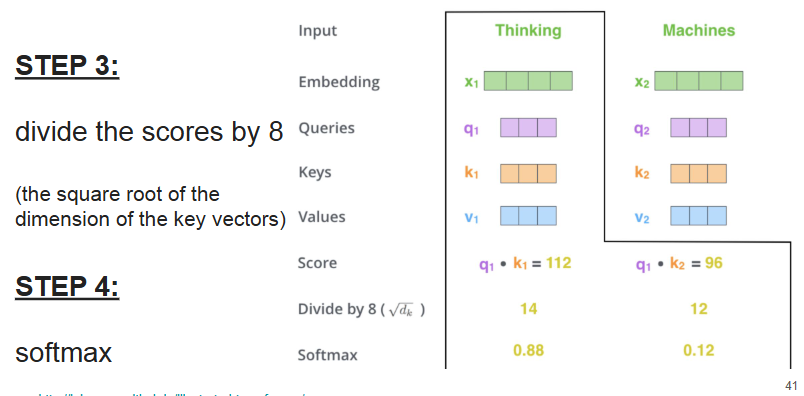
\includegraphics[width=0.8\textwidth]{figures/lecture04_scaled_dot_product_attention.png}
    \caption{Scaled dot-product attention: scores масштабируются и нормируются softmax-ом.}
\end{figure}

\subsection{Self-Attention в матричной форме}

Для всей последовательности можно собрать матрицы:

\[
X \in \mathbb{R}^{n \times d_{model}}.
\]

Тогда:

\[
Q = XW^Q,
\]

\[
K = XW^K,
\]

\[
V = XW^V.
\]

Матрица attention scores:

\[
QK^\top.
\]

После масштабирования:

\[
\frac{QK^\top}{\sqrt{d_k}}.
\]

Attention weights:

\[
A =
\operatorname{softmax}
\left(
\frac{QK^\top}{\sqrt{d_k}}
\right).
\]

Здесь softmax применяется построчно.

Итоговый выход:

\[
Z =
AV.
\]

Полная формула:

\[
\operatorname{Attention}(Q,K,V)
=
\operatorname{softmax}
\left(
\frac{QK^\top}{\sqrt{d_k}}
\right)V.
\]

Это одна из главных формул Transformer.

\subsection{Почему self-attention полезен}

Self-attention имеет несколько важных свойств.

\subsubsection{Короткий путь между позициями}

В RNN информация от первого токена до последнего должна пройти через много recurrent steps.

В self-attention любая позиция может напрямую обратиться к любой другой позиции за один слой.

Поэтому path length между любыми двумя позициями:

\[
O(1)
\]

внутри одного attention layer.

\subsubsection{Параллелизация}

RNN обрабатывает последовательность последовательно:

\[
h_t = f(h_{t-1}, x_t).
\]

Следовательно, состояние \(h_t\) нельзя посчитать до \(h_{t-1}\).

Transformer не имеет такой зависимости внутри encoder self-attention: все позиции слоя можно обрабатывать параллельно.

\subsubsection{Контекстуальные представления}

После self-attention представление каждого токена зависит от всей последовательности. Поэтому одно и то же слово может иметь разные векторы в разных контекстах.

\subsection{Multi-Head Attention}

Обычный attention даёт одну взвешенную сумму value-векторов.

Но одной attention-головы может быть недостаточно: разные типы связей в предложении могут требовать разных attention patterns.

\textbf{Multi-head attention} запускает несколько attention-механизмов параллельно.

Для каждой головы \(r\):

\[
Q_r = XW_r^Q,
\]

\[
K_r = XW_r^K,
\]

\[
V_r = XW_r^V.
\]

Затем:

\[
head_r
=
\operatorname{Attention}(Q_r,K_r,V_r).
\]

Если голов \(H\), получаем:

\[
head_1, head_2, \dots, head_H.
\]

Они конкатенируются:

\[
\operatorname{Concat}(head_1,\dots,head_H),
\]

а затем применяется выходная линейная проекция:

\[
\operatorname{MultiHead}(Q,K,V)
=
\operatorname{Concat}(head_1,\dots,head_H)W^O.
\]

\subsection{Зачем нужен Multi-Head Attention}

Multi-head attention полезен потому, что разные головы могут смотреть на разные типы отношений:

\begin{itemize}
    \item синтаксические зависимости;
    \item согласование местоимений;
    \item локальный контекст;
    \item дальний контекст;
    \item связи между объектом и действием;
    \item связи между частями фразы.
\end{itemize}

Иными словами, одна голова может фокусироваться на одном типе паттернов, другая --- на другом.

В лекции multi-head attention описан как:

\begin{quote}
parallel attention layers with different linear transformations on input and output.
\end{quote}

То есть это несколько attention layers, работающих параллельно с разными обучаемыми проекциями.

\subsection{Attention vs Multi-Head Attention}

\begin{table}[H]
\centering
\begin{tabular}{p{0.4\textwidth} p{0.5\textwidth}}
\toprule
\textbf{Attention} & \textbf{Multi-Head Attention} \\
\midrule
Одна weighted average по value-векторам. &
Несколько attention-механизмов параллельно. \\

Одна мера сходства между токенами. &
Несколько разных обучаемых пространств сходства. \\

Может ловить один доминирующий тип связей. &
Может одновременно ловить разные типы зависимостей. \\

Выход сразу используется дальше. &
Выходы голов конкатенируются и проецируются через \(W^O\). \\
\bottomrule
\end{tabular}
\caption{Сравнение обычного attention и multi-head attention.}
\end{table}

\subsection{Positional Encoding}

Self-attention сам по себе не знает порядок токенов.

Если переставить токены в последовательности, то механизм attention без дополнительной информации не имеет встроенного способа понять, какая позиция была первой, второй и т.д.

Поэтому в Transformer добавляется \textbf{positional encoding}.

Идея:

\[
\text{input representation}
=
\text{token embedding}
+
\text{positional encoding}.
\]

То есть для токена \(x_i\):

\[
\tilde{x}_i = x_i + p_i,
\]

где \(p_i\) --- positional encoding позиции \(i\).

\subsection{Требования к positional encoding}

В лекции перечислены требования:

\begin{itemize}
    \item positional encoding должен быть уникальным для каждой позиции;
    \item расстояние между одинаковыми позициями должно сохраняться для последовательностей разной длины;
    \item желательно, чтобы encoding был детерминированным;
    \item желательно, чтобы он работал с последовательностями длиннее тех, что встречались при обучении.
\end{itemize}

\subsection{Sinusoidal positional encoding}

В классическом Transformer используется синусоидальный positional encoding.

Для позиции \(pos\) и измерения \(i\):

\[
PE_{(pos, 2i)}
=
\sin
\left(
\frac{pos}{10000^{2i/d_{model}}}
\right),
\]

\[
PE_{(pos, 2i+1)}
=
\cos
\left(
\frac{pos}{10000^{2i/d_{model}}}
\right).
\]

Каждая размерность positional encoding соответствует синусоиде определённой частоты.

Длины волн образуют геометрическую прогрессию от:

\[
2\pi
\]

до примерно:

\[
2\pi \cdot 10000.
\]

Почему используются \(\sin\) и \(\cos\):

\begin{itemize}
    \item encoding детерминированный;
    \item можно вычислять позиции, не встречавшиеся при обучении;
    \item относительные сдвиги между позициями имеют регулярную структуру;
    \item разные частоты позволяют кодировать как локальные, так и дальние позиционные отношения.
\end{itemize}

% Слайд 65. Positional Encoding: почему используются sin и cos.
\begin{figure}[H]
    \centering
    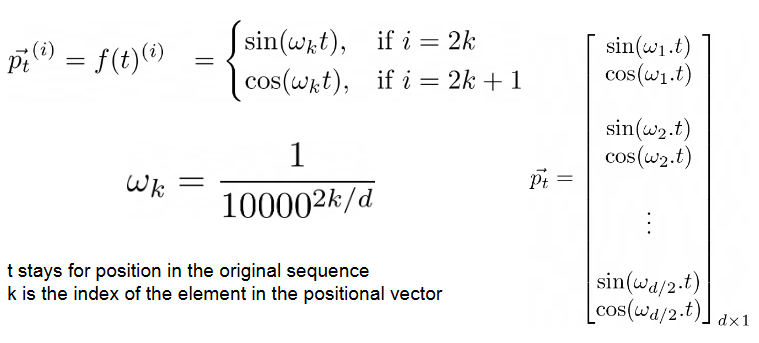
\includegraphics[width=0.85\textwidth]{figures/lecture04_positional_encoding_sincos.png}
    \caption{Sinusoidal positional encoding: разные измерения используют синусы и косинусы разных частот.}
\end{figure}

\subsection{Layer Normalization}

\textbf{Layer Normalization} --- нормализация активаций внутри одного объекта по его признакам.

Если есть вектор признаков:

\[
x = (x_1, x_2, \dots, x_d),
\]

то считаются среднее и дисперсия по координатам этого вектора:

\[
\mu =
\frac{1}{d}
\sum_{i=1}^{d} x_i,
\]

\[
\sigma^2 =
\frac{1}{d}
\sum_{i=1}^{d} (x_i - \mu)^2.
\]

Нормированный вектор:

\[
\hat{x}_i =
\frac{x_i - \mu}{\sqrt{\sigma^2 + \epsilon}}.
\]

Затем применяются обучаемые параметры масштаба и сдвига:

\[
y_i = \gamma_i \hat{x}_i + \beta_i.
\]

LayerNorm помогает стабилизировать обучение глубоких сетей.

\subsection{LayerNorm vs BatchNorm}

BatchNorm нормализует активации по batch dimension. Это хорошо работает во многих computer vision задачах, но может быть менее удобно для последовательностей переменной длины и autoregressive generation.

LayerNorm нормализует признаки внутри одного примера. Поэтому он лучше подходит для Transformer и NLP-задач.

\begin{table}[H]
\centering
\begin{tabular}{p{0.45\textwidth} p{0.45\textwidth}}
\toprule
\textbf{BatchNorm} & \textbf{LayerNorm} \\
\midrule
Нормализация по batch. &
Нормализация по признакам одного объекта. \\

Зависит от статистик батча. &
Не зависит от других объектов в батче. \\

Часто используется в CNN. &
Часто используется в Transformer. \\

Может быть неудобен для autoregressive моделей. &
Удобен для последовательностей и генерации. \\
\bottomrule
\end{tabular}
\caption{Сравнение BatchNorm и LayerNorm.}
\end{table}

\subsection{Residual connections в Transformer}

Хотя в презентации основной акцент сделан на attention и normalization, в стандартном Transformer каждый подслой используется вместе с residual connection.

Типичная структура:

\[
x \rightarrow \operatorname{Sublayer}(x),
\]

\[
y = \operatorname{LayerNorm}(x + \operatorname{Sublayer}(x)).
\]

Residual connection помогает градиентам проходить через глубокую сеть и делает обучение стабильнее.

Для encoder block это обычно:

\[
z = \operatorname{LayerNorm}(x + \operatorname{SelfAttention}(x)),
\]

\[
r = \operatorname{LayerNorm}(z + \operatorname{FeedForward}(z)).
\]

\subsection{Feed-Forward Network}

В каждом encoder и decoder block есть позиционная feed-forward сеть.

Она применяется независимо к каждой позиции:

\[
FFN(x) = W_2 \sigma(W_1 x + b_1) + b_2.
\]

Обычно:

\[
d_{ff} > d_{model}.
\]

То есть сначала размерность расширяется, затем снова уменьшается до \(d_{model}\).

Self-attention смешивает информацию между позициями, а feed-forward network преобразует представление каждой позиции отдельно.

\subsection{Decoder Side}

Decoder Transformer также состоит из нескольких блоков.

Каждый decoder block обычно содержит:

\begin{enumerate}
    \item masked self-attention;
    \item encoder-decoder attention;
    \item feed-forward network.
\end{enumerate}

\subsection{Masked Self-Attention}

В decoder-е нельзя позволять позиции \(t\) смотреть на будущие target tokens:

\[
y_{t+1}, y_{t+2}, \dots
\]

Иначе модель во время обучения увидит правильное будущее и задача генерации станет некорректной.

Поэтому используется \textbf{mask}.

Masked self-attention разрешает токену \(t\) смотреть только на:

\[
y_1, y_2, \dots, y_t.
\]

То есть запрещены связи:

\[
t \rightarrow j, \quad j > t.
\]

В матрице attention это реализуется добавлением \(-\infty\) к запрещённым позициям перед softmax:

\[
\operatorname{softmax}
\left(
\frac{QK^\top}{\sqrt{d_k}} + M
\right),
\]

где:

\[
M_{ij} =
\begin{cases}
0, & j \leq i, \\
-\infty, & j > i.
\end{cases}
\]

После softmax будущие позиции получают нулевой вес.

% Слайд 76. Decoder side: появляется mask для запрета внимания на будущие токены.
\begin{figure}[H]
    \centering
    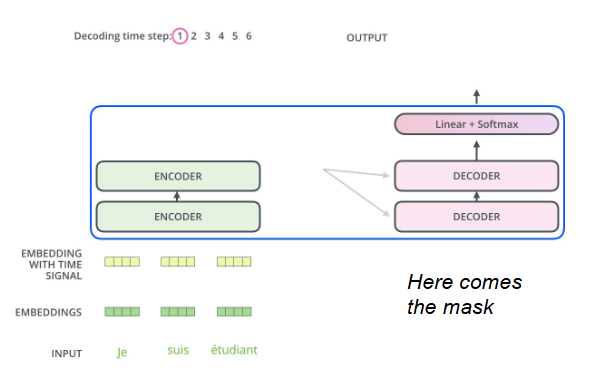
\includegraphics[width=0.85\textwidth]{figures/lecture04_decoder_mask.png}
    \caption{Masked self-attention в decoder-е запрещает смотреть на будущие токены.}
\end{figure}

\subsection{Encoder-Decoder Attention}

После masked self-attention decoder использует encoder-decoder attention.

В этом attention:

\begin{itemize}
    \item queries берутся из decoder-а;
    \item keys и values берутся из выходов encoder-а.
\end{itemize}

То есть decoder на каждом шаге спрашивает:

\[
\text{какая часть source sequence сейчас важна для генерации target token?}
\]

Формально:

\[
Q = H_{dec}W^Q,
\]

\[
K = H_{enc}W^K,
\]

\[
V = H_{enc}W^V.
\]

Затем:

\[
\operatorname{Attention}(Q,K,V)
=
\operatorname{softmax}
\left(
\frac{QK^\top}{\sqrt{d_k}}
\right)V.
\]

Это аналог attention из seq2seq, но встроенный в Transformer.

\subsection{Final Linear and Softmax Layer}

На выходе decoder-а получаем вектор для каждой позиции target sequence.

Чтобы получить распределение по словарю, применяется linear layer:

\[
o_t = W_{vocab} h_t + b_{vocab}.
\]

Затем softmax:

\[
P(y_t = w \mid y_{<t}, x)
=
\frac{
\exp(o_{t,w})
}{
\sum_{w' \in \mathcal{V}}
\exp(o_{t,w'})
}.
\]

Модель обучается предсказывать следующий токен в target sequence.

\subsection{Сравнение RNN, CNN и Transformer}

\begin{table}[H]
\centering
\begin{tabular}{p{0.28\textwidth} p{0.32\textwidth} p{0.32\textwidth}}
\toprule
\textbf{Архитектура} & \textbf{Плюсы} & \textbf{Минусы} \\
\midrule

RNN &
Естественно моделирует последовательность, учитывает порядок. &
Плохо параллелится, длинный путь между дальними токенами, vanishing gradients. \\

CNN &
Хорошо ловит локальные паттерны, параллелится лучше RNN. &
Для дальних зависимостей нужны большие окна или много слоёв. \\

Transformer &
Короткий путь между любыми позициями, хорошо параллелится, моделирует дальние зависимости. &
Self-attention имеет квадратичную сложность по длине последовательности. \\

\bottomrule
\end{tabular}
\caption{Сравнение RNN, CNN и Transformer для обработки последовательностей.}
\end{table}

\subsection{Сложность self-attention}

Для последовательности длины \(n\) attention scores считаются для всех пар токенов:

\[
QK^\top \in \mathbb{R}^{n \times n}.
\]

Поэтому сложность по времени и памяти относительно длины последовательности:

\[
O(n^2).
\]

Это важное ограничение Transformer для очень длинных последовательностей.

Однако для умеренных длин Transformer очень эффективен, потому что вычисления хорошо параллелятся на GPU.

\subsection{Research challenges}

В лекции упоминаются свойства и исследовательские вызовы attention-подходов:

\begin{itemize}
    \item constant path length between any two positions;
    \item unbounded memory;
    \item trivial parallelization per layer;
    \item modeling self-similarity;
    \item relative attention;
    \item расширение attention-подходов на графы.
\end{itemize}

Ключевая идея: attention является более общим механизмом связывания элементов структуры. Его можно применять не только к текстам, но и к другим данным, где важны отношения между элементами.

\subsection{Главные выводы}

\begin{itemize}
    \item Transformer основан на self-attention и не использует RNN или CNN как основной механизм обработки последовательности.
    \item Self-attention позволяет каждому токену учитывать все остальные токены последовательности.
    \item Для каждого токена строятся Query, Key и Value векторы.
    \item Главная формула scaled dot-product attention:
    \[
    \operatorname{Attention}(Q,K,V)
    =
    \operatorname{softmax}
    \left(
    \frac{QK^\top}{\sqrt{d_k}}
    \right)V.
    \]

    \item Multi-head attention запускает несколько attention-механизмов параллельно.
    \item Positional encoding нужен, потому что self-attention сам по себе не знает порядок токенов.
    \item Sinusoidal positional encoding использует синусы и косинусы разных частот.
    \item LayerNorm стабилизирует обучение Transformer.
    \item Decoder использует masked self-attention, чтобы не смотреть в будущие target tokens.
    \item Transformer хорошо параллелится и имеет короткий путь между любыми позициями.
\end{itemize}

\subsection{Что важно помнить к экзамену}

\begin{enumerate}
    \item Attention в seq2seq:
    \[
    e_{t,i}=s_t^\top h_i,
    \]
    \[
    \alpha^t=\operatorname{softmax}(e^t),
    \]
    \[
    a_t=\sum_{i=1}^{N}\alpha_i^t h_i.
    \]

    \item Transformer предложен в статье \textit{Attention is All You Need}.

    \item В Transformer нет рекуррентности: основная операция --- self-attention.

    \item Encoder block состоит из:
    \begin{itemize}
        \item self-attention;
        \item feed-forward network;
        \item residual connections;
        \item layer normalization.
    \end{itemize}

    \item Query, Key, Value:
    \[
    Q=XW^Q,
    \quad
    K=XW^K,
    \quad
    V=XW^V.
    \]

    \item Scaled dot-product attention:
    \[
    \operatorname{Attention}(Q,K,V)
    =
    \operatorname{softmax}
    \left(
    \frac{QK^\top}{\sqrt{d_k}}
    \right)V.
    \]

    \item Зачем делить на \(\sqrt{d_k}\): чтобы стабилизировать значения перед softmax.

    \item Multi-head attention:
    \[
    head_r =
    \operatorname{Attention}(Q_r,K_r,V_r),
    \]
    \[
    \operatorname{MultiHead}
    =
    \operatorname{Concat}(head_1,\dots,head_H)W^O.
    \]

    \item Positional encoding добавляется к token embeddings:
    \[
    \tilde{x}_i = x_i + p_i.
    \]

    \item Sinusoidal positional encoding:
    \[
    PE_{(pos, 2i)}
    =
    \sin
    \left(
    \frac{pos}{10000^{2i/d_{model}}}
    \right),
    \]
    \[
    PE_{(pos, 2i+1)}
    =
    \cos
    \left(
    \frac{pos}{10000^{2i/d_{model}}}
    \right).
    \]

    \item LayerNorm:
    \[
    \hat{x}_i =
    \frac{x_i-\mu}{\sqrt{\sigma^2+\epsilon}},
    \]
    \[
    y_i = \gamma_i \hat{x}_i + \beta_i.
    \]

    \item Masked self-attention запрещает decoder-у смотреть на будущие токены.

    \item Главный плюс Transformer относительно RNN:
    \[
    \text{короткий путь между любыми двумя позициями и хорошая параллелизация}.
    \]

    \item Главный минус классического self-attention:
    \[
    O(n^2)
    \]
    по длине последовательности.
\end{enumerate}
```








```latex
\section{Лекция 5. Transfer Learning, BERT, GPT}

\subsection{План лекции}

В этой лекции рассматриваются:

\begin{itemize}
    \item повторение self-attention и Transformer;
    \item multi-head attention;
    \item positional encoding;
    \item layer normalization;
    \item transfer learning в NLP;
    \item OpenAI Transformer / GPT-подход;
    \item ELMo;
    \item BERT;
    \item pre-training и fine-tuning;
    \item BERT tokenization.
\end{itemize}

Главная идея лекции: современные NLP-модели обычно сначала обучаются на большой self-supervised задаче, например language modeling, а затем дообучаются на конкретную downstream-задачу. Это называется transfer learning.

\subsection{Повторение: self-attention}

Self-attention позволяет каждому токену последовательности учитывать остальные токены той же последовательности.

Для входной матрицы embeddings:

\[
X \in \mathbb{R}^{n \times d_{model}}
\]

строятся три матрицы:

\[
Q = XW^Q,
\]

\[
K = XW^K,
\]

\[
V = XW^V.
\]

Здесь:

\begin{itemize}
    \item \(Q\) --- queries;
    \item \(K\) --- keys;
    \item \(V\) --- values;
    \item \(W^Q, W^K, W^V\) --- обучаемые матрицы.
\end{itemize}

Для каждой пары токенов считается score:

\[
QK^\top.
\]

Затем scores масштабируются:

\[
\frac{QK^\top}{\sqrt{d_k}}.
\]

Деление на \(\sqrt{d_k}\) нужно, чтобы значения перед softmax не становились слишком большими при большой размерности key-векторов.

После этого применяется softmax:

\[
A =
\operatorname{softmax}
\left(
\frac{QK^\top}{\sqrt{d_k}}
\right).
\]

Итоговый выход self-attention:

\[
Z = AV.
\]

Главная формула:

\[
\operatorname{Attention}(Q,K,V)
=
\operatorname{softmax}
\left(
\frac{QK^\top}{\sqrt{d_k}}
\right)V.
\]

% Слайд 4. Матричная формула self-attention: softmax(QK^T / sqrt(d_k))V.
\begin{figure}[H]
    \centering
    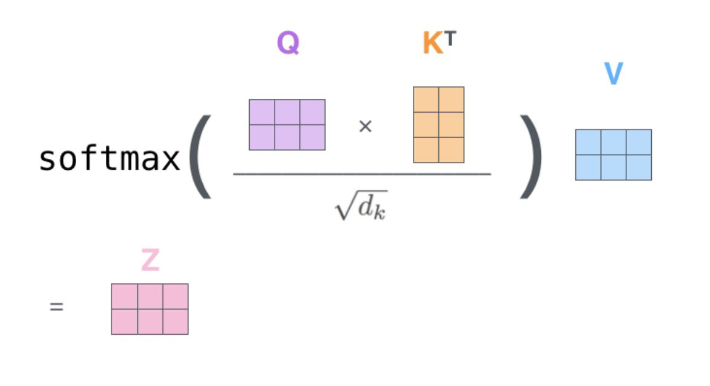
\includegraphics[width=0.75\textwidth]{figures/lecture05_self_attention_matrix.png}
    \caption{Матричная форма scaled dot-product attention.}
\end{figure}

\subsection{Multi-Head Attention}

В multi-head attention несколько attention-механизмов запускаются параллельно.

Для каждой головы \(r\):

\[
Q_r = XW_r^Q,
\]

\[
K_r = XW_r^K,
\]

\[
V_r = XW_r^V.
\]

Затем считается:

\[
head_r
=
\operatorname{Attention}(Q_r,K_r,V_r).
\]

Если всего \(H\) голов, то:

\[
head_1, head_2, \dots, head_H
\]

конкатенируются:

\[
\operatorname{Concat}(head_1,\dots,head_H),
\]

а затем проецируются обучаемой матрицей \(W^O\):

\[
\operatorname{MultiHead}(Q,K,V)
=
\operatorname{Concat}(head_1,\dots,head_H)W^O.
\]

Смысл multi-head attention: разные головы могут смотреть на разные типы зависимостей в тексте.

Например:

\begin{itemize}
    \item одна голова может отслеживать локальный контекст;
    \item другая --- синтаксические связи;
    \item третья --- связи между местоимением и объектом;
    \item четвёртая --- дальние зависимости.
\end{itemize}

% Слайд 8. Общая схема multi-head attention: несколько голов, конкатенация и выходная проекция.
\begin{figure}[H]
    \centering
    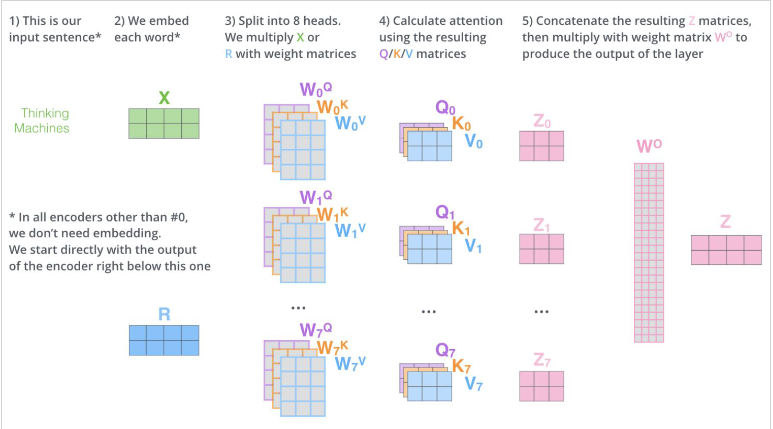
\includegraphics[width=0.9\textwidth]{figures/lecture05_multi_head_attention.png}
    \caption{Multi-head attention: несколько attention-голов работают параллельно, затем их выходы объединяются.}
\end{figure}

\subsection{Positional Encoding}

Self-attention сам по себе не содержит информации о порядке токенов. Поэтому Transformer добавляет к token embeddings positional encoding.

Для токена в позиции \(i\):

\[
\tilde{x}_i = x_i + p_i,
\]

где:

\begin{itemize}
    \item \(x_i\) --- embedding токена;
    \item \(p_i\) --- positional encoding;
    \item \(\tilde{x}_i\) --- итоговое входное представление.
\end{itemize}

Positional encoding нужен, чтобы модель могла различать предложения с одинаковыми словами, но разным порядком.

Например:

\[
\text{dog bites man}
\]

и

\[
\text{man bites dog}
\]

содержат одинаковые слова, но имеют разный смысл.

В классическом Transformer используется sinusoidal positional encoding:

\[
PE_{(pos, 2i)}
=
\sin
\left(
\frac{pos}{10000^{2i/d_{model}}}
\right),
\]

\[
PE_{(pos, 2i+1)}
=
\cos
\left(
\frac{pos}{10000^{2i/d_{model}}}
\right).
\]

Каждая размерность positional encoding соответствует синусоиде своей частоты.

% Слайд 10. Positional encoding добавляется к token embeddings перед Transformer.
\begin{figure}[H]
    \centering
    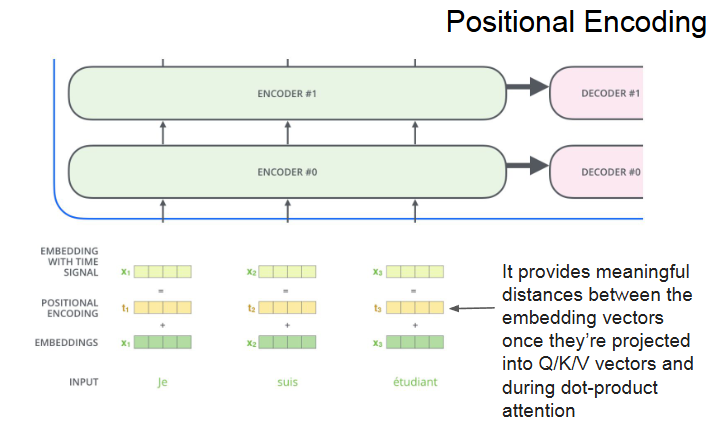
\includegraphics[width=0.85\textwidth]{figures/lecture05_positional_encoding.png}
    \caption{Positional encoding добавляет информацию о позиции токена к его embedding.}
\end{figure}

\subsection{Layer Normalization}

В Transformer активно используется связка:

\[
\text{Add \& Normalize}.
\]

Она означает residual connection и layer normalization.

Если есть вход \(x\) и некоторый подслой \(\operatorname{Sublayer}(x)\), то:

\[
y =
\operatorname{LayerNorm}
\left(
x + \operatorname{Sublayer}(x)
\right).
\]

Residual connection помогает передавать градиенты через глубокую сеть:

\[
x + \operatorname{Sublayer}(x).
\]

Layer normalization стабилизирует распределение активаций.

Для вектора:

\[
x = (x_1, x_2, \dots, x_d)
\]

среднее:

\[
\mu =
\frac{1}{d}
\sum_{i=1}^{d} x_i,
\]

дисперсия:

\[
\sigma^2 =
\frac{1}{d}
\sum_{i=1}^{d}
(x_i-\mu)^2.
\]

Нормировка:

\[
\hat{x}_i =
\frac{x_i-\mu}
{\sqrt{\sigma^2+\epsilon}}.
\]

После этого применяются обучаемые scale и shift:

\[
y_i = \gamma_i \hat{x}_i + \beta_i.
\]

\subsection{Transformer recap}

Классический Transformer состоит из encoder stack и decoder stack.

Encoder block содержит:

\begin{itemize}
    \item multi-head self-attention;
    \item add \& norm;
    \item feed-forward network;
    \item add \& norm.
\end{itemize}

Decoder block содержит:

\begin{itemize}
    \item masked multi-head self-attention;
    \item add \& norm;
    \item encoder-decoder attention;
    \item add \& norm;
    \item feed-forward network;
    \item add \& norm.
\end{itemize}

На выходе decoder-а применяются:

\[
\text{Linear} \rightarrow \text{Softmax}.
\]

Это даёт распределение вероятностей по словарю.

% Слайд 13. Полная схема Transformer: encoder stack, decoder stack, Add & Norm, FFN, attention layers.
\begin{figure}[H]
    \centering
    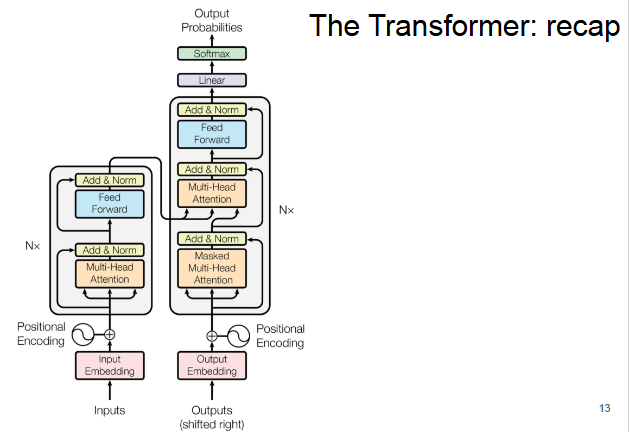
\includegraphics[width=0.75\textwidth]{figures/lecture05_transformer_recap.png}
    \caption{Общая схема Transformer с encoder и decoder stack.}
\end{figure}

\subsection{Transfer Learning в NLP}

\textbf{Transfer learning} --- подход, при котором модель сначала обучается на одной большой общей задаче, а затем используется или дообучается для других задач.

В NLP типичный сценарий:

\begin{enumerate}
    \item pre-training на огромном корпусе без ручных меток;
    \item fine-tuning на конкретной downstream-задаче.
\end{enumerate}

Downstream-задачи:

\begin{itemize}
    \item классификация текста;
    \item sentiment analysis;
    \item question answering;
    \item textual entailment;
    \item similarity;
    \item named entity recognition;
    \item machine translation;
    \item multiple choice.
\end{itemize}

Главное преимущество: для pre-training можно использовать огромные неразмеченные корпуса, а для конкретной задачи нужно намного меньше размеченных данных.

\subsection{OpenAI Transformer и GPT-подход}

Encoder-decoder Transformer хорошо подходит для машинного перевода. Но для многих задач, например sentence classification, можно использовать только часть Transformer.

OpenAI Transformer использует decoder-only подход.

Отличия от vanilla Transformer:

\begin{itemize}
    \item нет encoder-а;
    \item decoder layers не имеют encoder-decoder attention sublayer;
    \item модель обучается предсказывать следующий токен;
    \item pre-training проводится на больших неразмеченных корпусах.
\end{itemize}

То есть модель обучается как language model:

\[
P(x_1, x_2, \dots, x_T)
=
\prod_{t=1}^{T}
P(x_t \mid x_{<t}).
\]

Или в задаче next-token prediction:

\[
P(x_t \mid x_1, \dots, x_{t-1}).
\]

Так как модель обучается предсказывать следующий токен, она должна научиться представлять язык, синтаксис, семантику и типичные зависимости в тексте.

После pre-training модель можно использовать для downstream-задач.

\subsection{Fine-tuning OpenAI Transformer}

После pre-training слои модели уже умеют разумно обрабатывать язык. Для downstream-задачи можно добавить небольшую task-specific голову.

Например, для классификации текста:

\[
\text{text}
\rightarrow
\text{OpenAI Transformer}
\rightarrow
\text{FFNN + Softmax}
\rightarrow
\text{class probabilities}.
\]

Для spam classification выход может быть:

\[
P(\text{Spam} \mid x),
\quad
P(\text{Not Spam} \mid x).
\]

% Слайд 20. Использование pretrained OpenAI Transformer для sentence classification.
\begin{figure}[H]
    \centering
    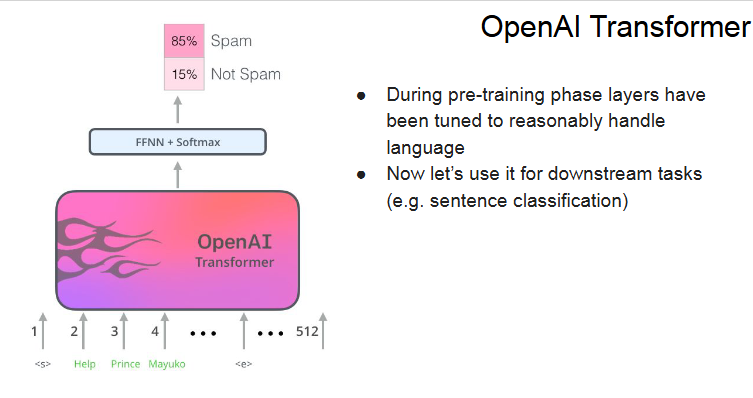
\includegraphics[width=0.85\textwidth]{figures/lecture05_openai_transformer_finetuning.png}
    \caption{Fine-tuning OpenAI Transformer для downstream-задачи классификации.}
\end{figure}

\subsection{Input transformations для разных задач}

Одна и та же pretrained Transformer-модель может использоваться для разных задач, если правильно преобразовать вход.

Примеры:

\begin{itemize}
    \item \textbf{Classification}: один текст подаётся в модель, затем используется выход для классификации.
    \item \textbf{Entailment}: подаются premise и hypothesis, разделённые специальным delimiter token.
    \item \textbf{Similarity}: подаются две версии пары текстов, затем их представления сравниваются.
    \item \textbf{Multiple choice}: для каждого варианта ответа формируется отдельная последовательность context + answer, затем выбирается лучший вариант.
\end{itemize}

% Слайд 21. Преобразование входов для classification, entailment, similarity и multiple choice.
\begin{figure}[H]
    \centering
    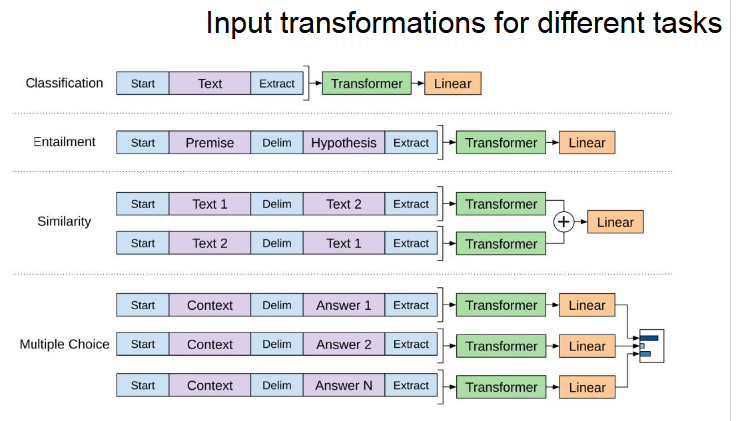
\includegraphics[width=0.95\textwidth]{figures/lecture05_input_transformations.png}
    \caption{Input transformations позволяют применять одну pretrained модель к разным NLP-задачам.}
\end{figure}

\subsection{ELMo: contextualized word embeddings}

До контекстуальных embeddings одно слово обычно имело один фиксированный вектор.

Например, слово:

\[
\text{stick}
\]

имело бы один embedding независимо от контекста.

Но слово может иметь разные значения:

\[
\text{stick to the plan},
\]

\[
\text{wooden stick},
\]

\[
\text{stick in the mud}.
\]

\textbf{ELMo} решает эту проблему.

ELMo означает:

\[
\text{Embeddings from Language Models}.
\]

Главная идея:

\begin{quote}
Давать слову embedding, зависящий от контекста, в котором оно используется.
\end{quote}

То есть:

\[
\text{embedding}(\text{word})
\]

становится функцией всего предложения:

\[
\text{embedding}(w_i \mid w_1,\dots,w_n).
\]

\subsection{Bidirectional Language Models}

ELMo использует bidirectional LSTM, обученную на language modeling task.

Bidirectional language model состоит из:

\begin{itemize}
    \item forward language model;
    \item backward language model.
\end{itemize}

Forward LM моделирует вероятность последовательности слева направо:

\[
P(t_1,t_2,\dots,t_N)
=
\prod_{k=1}^{N}
P(t_k \mid t_1,\dots,t_{k-1}).
\]

Backward LM моделирует вероятность справа налево:

\[
P(t_1,t_2,\dots,t_N)
=
\prod_{k=1}^{N}
P(t_k \mid t_{k+1},\dots,t_N).
\]

Идея: слово получает информацию и из левого, и из правого контекста.

% Слайд 28. Bidirectional Language Models: forward и backward LMs на LSTM.
\begin{figure}[H]
    \centering
    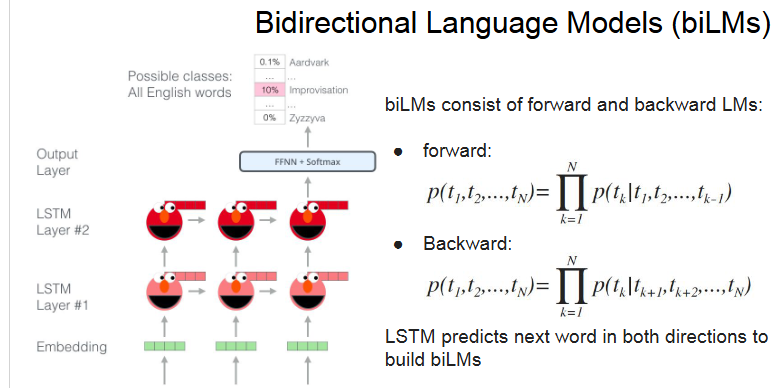
\includegraphics[width=0.85\textwidth]{figures/lecture05_elmo_bilm.png}
    \caption{ELMo использует bidirectional language model: forward и backward LSTM.}
\end{figure}

\subsection{ELMo pipeline}

ELMo представляет слово как комбинацию hidden states разных слоёв biLSTM.

Пусть для токена \(k\) есть представления на разных слоях:

\[
h_{k,0}, h_{k,1}, \dots, h_{k,L}.
\]

Тогда ELMo embedding можно представить как взвешенную сумму:

\[
\operatorname{ELMo}_k
=
\gamma
\sum_{j=0}^{L}
s_j h_{k,j}.
\]

Здесь:

\begin{itemize}
    \item \(s_j\) --- обучаемые task-specific веса слоёв;
    \item \(\gamma\) --- обучаемый scale parameter;
    \item \(h_{k,j}\) --- представление токена \(k\) на слое \(j\).
\end{itemize}

Разные слои могут кодировать разные типы информации:

\begin{itemize}
    \item нижние слои чаще ловят синтаксис;
    \item верхние слои чаще ловят семантику.
\end{itemize}

ELMo можно добавить почти в любую нейронную NLP-модель через конкатенацию с обычным embedding layer:

\[
x_i^{new}
=
[x_i; \operatorname{ELMo}_i].
\]

\subsection{BERT}

\textbf{BERT} расшифровывается как:

\[
\text{Bidirectional Encoder Representations from Transformers}.
\]

BERT использует encoder-only Transformer.

В отличие от GPT-like decoder-only моделей, BERT смотрит на контекст с обеих сторон. Поэтому он хорошо подходит для задач понимания текста:

\begin{itemize}
    \item sentence classification;
    \item question answering;
    \item named entity recognition;
    \item entailment;
    \item similarity.
\end{itemize}

Для классификации текста схема выглядит так:

\[
\text{text}
\rightarrow
\text{BERT}
\rightarrow
\text{classifier}
\rightarrow
\text{prediction}.
\]

% Слайд 35. BERT для классификации текста: входной текст -> BERT -> classifier -> prediction.
\begin{figure}[H]
    \centering
    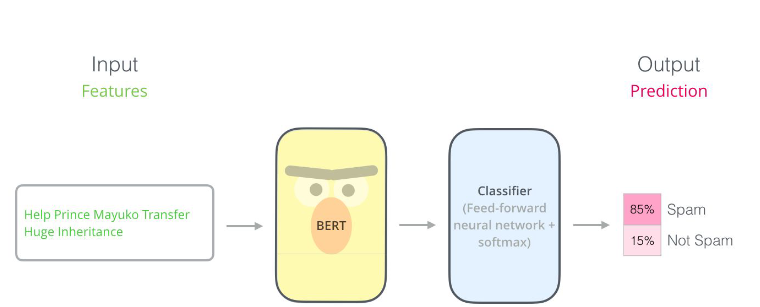
\includegraphics[width=0.85\textwidth]{figures/lecture05_bert_classification.png}
    \caption{BERT как encoder для downstream-классификации.}
\end{figure}

\subsection{BERT Base и BERT Large}

В лекции сравниваются варианты BERT Base и BERT Large.

\begin{table}[H]
\centering
\begin{tabular}{lccc}
\toprule
\textbf{Модель} & \textbf{Encoders} & \textbf{Units in FFN} & \textbf{Attention Heads} \\
\midrule
Transformer из лекции & 6 & 512 & 8 \\
BERT Base & 12 & 768 & 12 \\
BERT Large & 24 & 1024 & 16 \\
\bottomrule
\end{tabular}
\caption{Сравнение размеров Transformer, BERT Base и BERT Large.}
\end{table}

BERT Large глубже и шире, поэтому обычно мощнее, но требует больше памяти и вычислений.

\subsection{BERT inputs}

BERT получает последовательность токенов фиксированной максимальной длины, например 512.

Для классификации в начало последовательности добавляется специальный токен:

\[
[\text{CLS}].
\]

Например:

\[
[\text{CLS}], \text{Help}, \text{Prince}, \text{Mayuko}, \dots
\]

Каждая позиция на выходе BERT выдаёт вектор.

Для sentence classification обычно берётся вектор первой позиции, соответствующий:

\[
[\text{CLS}].
\]

Этот вектор используется как представление всего текста:

\[
h_{CLS}.
\]

Затем:

\[
\hat{y}
=
\operatorname{softmax}(Wh_{CLS}+b).
\]

То есть \(h_{CLS}\) подаётся в классификатор.

\subsection{Почему BERT особенный}

Главная особенность BERT --- bidirectional pre-training.

Обычная autoregressive language model предсказывает следующий токен по левому контексту:

\[
P(x_t \mid x_1,\dots,x_{t-1}).
\]

BERT хочет использовать контекст с обеих сторон:

\[
x_1,\dots,x_{t-1}
\quad \text{и} \quad
x_{t+1},\dots,x_n.
\]

Но если просто дать модели весь текст и попросить предсказывать токен, она увидит сам правильный токен.

Поэтому BERT использует masked language modeling.

\subsection{BERT pre-training}

BERT обучается на двух задачах:

\begin{enumerate}
    \item Masked Language Modeling;
    \item Next Sentence Prediction.
\end{enumerate}

\subsubsection{Masked Language Modeling}

В Masked Language Modeling часть токенов во входе заменяется на специальный токен:

\[
[\text{MASK}].
\]

Модель должна восстановить скрытые токены по контексту.

Пример:

\[
\text{The animal did not cross the street because it was too tired}
\]

может быть превращён в:

\[
\text{The animal did not cross the } [\text{MASK}] \text{ because it was too tired}.
\]

Модель должна предсказать:

\[
\text{street}.
\]

Преимущество MLM: модель может использовать и левый, и правый контекст.

\subsubsection{Next Sentence Prediction}

Чтобы BERT лучше понимал отношения между предложениями, добавляется задача:

\begin{quote}
Даны два предложения \(A\) и \(B\). Является ли \(B\) вероятным следующим предложением после \(A\)?
\end{quote}

Это бинарная классификация:

\[
y \in \{\text{IsNext}, \text{NotNext}\}.
\]

Эта задача полезна для:

\begin{itemize}
    \item question answering;
    \item natural language inference;
    \item задач на отношения между двумя предложениями.
\end{itemize}

\subsection{BERT fine-tuning}

После pre-training BERT можно дообучать для конкретных задач.

Общая схема:

\[
\text{pretrained BERT}
+
\text{small task-specific head}
\rightarrow
\text{fine-tuning}.
\]

Примеры:

\subsubsection{Text classification}

Используется выход токена \([\text{CLS}]\):

\[
h_{CLS}
\rightarrow
\text{Linear}
\rightarrow
\text{Softmax}.
\]

\subsubsection{Token classification}

Для задач вроде named entity recognition используется выход каждой позиции:

\[
h_1, h_2, \dots, h_n.
\]

Для каждого токена предсказывается метка:

\[
y_i = \operatorname{softmax}(Wh_i+b).
\]

\subsubsection{Question answering}

Для extractive QA модель предсказывает:

\[
p_{start}
\]

и

\[
p_{end},
\]

то есть начало и конец ответа в тексте.

\subsection{BERT как feature extractor}

BERT можно использовать не только для fine-tuning, но и как feature extractor.

В этом режиме:

\begin{itemize}
    \item BERT не дообучается;
    \item через него прогоняют текст;
    \item берут hidden states одного или нескольких слоёв;
    \item эти векторы используют как признаки для другой модели.
\end{itemize}

Например, для каждого токена можно взять:

\[
h_i^{(L)}
\]

из последнего слоя или конкатенацию нескольких последних слоёв.

Fine-tuning обычно даёт лучшее качество, но feature extraction может быть полезен, если мало ресурсов или нужно быстро получить признаки.

\subsection{BERT tokenization}

BERT использует WordPiece tokenization.

Идея: слова разбиваются на подсловные единицы.

Пример из лекции:

\[
\text{Unaffable}
\rightarrow
\text{un}, \text{\#\#aff}, \text{\#\#able}.
\]

Префикс:

\[
\text{\#\#}
\]

означает, что фрагмент не является началом слова.

Преимущества WordPiece:

\begin{itemize}
    \item можно обрабатывать редкие и неизвестные слова;
    \item словарь остаётся ограниченного размера;
    \item модель может работать с морфологически сложными словами;
    \item один и тот же словарь можно использовать для многих языков.
\end{itemize}

В лекции указано, что multilingual BERT использует один shared vocabulary для 104 языков:

\[
119\,547
\]

WordPiece units.

Также отмечается:

\begin{itemize}
    \item первые 106 символов --- специальные константы вроде PAD и UNK;
    \item \(36.5\%\) словаря --- non-initial word pieces;
    \item алфавит включает \(9997\) уникальных символов;
    \item символы представлены как word-initial и continuation symbols;
    \item остальные элементы словаря --- многосимвольные word pieces разной длины.
\end{itemize}

\subsection{Сравнение ELMo, GPT-like моделей и BERT}

\begin{table}[H]
\centering
\begin{tabular}{p{0.22\textwidth} p{0.32\textwidth} p{0.36\textwidth}}
\toprule
\textbf{Модель} & \textbf{Архитектура} & \textbf{Основная идея} \\
\midrule

ELMo &
BiLSTM language model. &
Контекстуальные embeddings из forward и backward LM. \\

OpenAI Transformer / GPT-like &
Decoder-only Transformer. &
Pre-training через next-token prediction, затем fine-tuning. \\

BERT &
Encoder-only Transformer. &
Bidirectional representations через masked language modeling. \\

\bottomrule
\end{tabular}
\caption{Сравнение основных transfer learning подходов в NLP.}
\end{table}

\subsection{Главные выводы}

\begin{itemize}
    \item Transfer learning стал ключевой идеей современного NLP.
    \item Модель сначала обучается на большой self-supervised задаче, затем дообучается на downstream-задаче.
    \item OpenAI Transformer использует decoder-only Transformer и next-token prediction.
    \item ELMo даёт контекстуальные word embeddings на основе bidirectional LSTM.
    \item BERT использует encoder-only Transformer.
    \item BERT обучается через Masked Language Modeling и Next Sentence Prediction.
    \item Для классификации в BERT обычно используется выход токена \([\text{CLS}]\).
    \item BERT можно использовать как fine-tuned модель или как feature extractor.
    \item WordPiece tokenization позволяет работать с редкими словами через подсловные единицы.
\end{itemize}

\subsection{Что важно помнить к экзамену}

\begin{enumerate}
    \item Формулу self-attention:
    \[
    \operatorname{Attention}(Q,K,V)
    =
    \operatorname{softmax}
    \left(
    \frac{QK^\top}{\sqrt{d_k}}
    \right)V.
    \]

    \item Что multi-head attention --- это несколько attention heads с разными линейными проекциями.

    \item Зачем нужен positional encoding:
    self-attention сам по себе не знает порядок токенов.

    \item Что такое transfer learning:
    \[
    \text{pre-training} \rightarrow \text{fine-tuning}.
    \]

    \item OpenAI Transformer / GPT-like подход:
    \[
    P(x_1,\dots,x_T)
    =
    \prod_{t=1}^{T}
    P(x_t \mid x_{<t}).
    \]

    \item ELMo:
    \[
    \operatorname{ELMo}_k
    =
    \gamma
    \sum_{j=0}^{L}
    s_j h_{k,j}.
    \]

    \item Forward LM:
    \[
    P(t_1,\dots,t_N)
    =
    \prod_{k=1}^{N}
    P(t_k \mid t_1,\dots,t_{k-1}).
    \]

    \item Backward LM:
    \[
    P(t_1,\dots,t_N)
    =
    \prod_{k=1}^{N}
    P(t_k \mid t_{k+1},\dots,t_N).
    \]

    \item BERT расшифровывается как:
    \[
    \text{Bidirectional Encoder Representations from Transformers}.
    \]

    \item BERT использует encoder-only Transformer.

    \item BERT pre-training состоит из:
    \begin{itemize}
        \item Masked Language Modeling;
        \item Next Sentence Prediction.
    \end{itemize}

    \item Для sentence classification используется вектор токена:
    \[
    [\text{CLS}].
    \]

    \item WordPiece tokenization:
    \[
    \text{Unaffable}
    \rightarrow
    \text{un}, \text{\#\#aff}, \text{\#\#able}.
    \]
\end{enumerate}
```
```latex
\section{Лекция 6. Contrastive Learning}

\subsection{План лекции}

В этой лекции рассматриваются:

\begin{itemize}
    \item self-supervised learning;
    \item pretext tasks;
    \item отличие generative и self-supervised learning;
    \item оценка self-supervised методов;
    \item pretext tasks на изображениях;
    \item contrastive representation learning;
    \item InfoNCE loss;
    \item SimCLR;
    \item MoCo;
    \item CPC.
\end{itemize}

Главная идея лекции: можно обучать полезные представления без ручной разметки. Для этого модель решает автоматически сгенерированную задачу, а затем полученные признаки используются в downstream-задачах.

\subsection{Self-supervised learning}

\textbf{Self-supervised learning} --- подход, при котором модель обучается без ручной разметки, но с supervised objective.

Ключевая идея:

\begin{itemize}
    \item настоящих human labels нет;
    \item labels генерируются автоматически из самих данных;
    \item модель решает вспомогательную задачу;
    \item цель не сама вспомогательная задача, а хорошие признаки для downstream-задач.
\end{itemize}

Такая вспомогательная задача называется \textbf{pretext task}.

Например, для изображения можно автоматически создать задачу:

\begin{itemize}
    \item предсказать угол поворота;
    \item восстановить скрытую часть изображения;
    \item собрать ``jigsaw puzzle'';
    \item раскрасить grayscale image.
\end{itemize}

Для каждой такой задачи labels можно получить автоматически. Например, если мы сами повернули изображение на \(90^\circ\), то label равен \(90^\circ\).

\subsection{Pretext task}

\textbf{Pretext task} --- искусственная задача, которая создаётся не ради итогового качества на этой задаче, а ради обучения полезного feature extractor.

Пусть есть много неразмеченных данных:

\[
x_1, x_2, \dots, x_N.
\]

Мы автоматически строим пары:

\[
(\tilde{x}_i, \tilde{y}_i),
\]

где:

\begin{itemize}
    \item \(\tilde{x}_i\) --- изменённый объект;
    \item \(\tilde{y}_i\) --- автоматически известная метка.
\end{itemize}

После этого обучаем модель:

\[
f_\theta(\tilde{x}) \rightarrow \tilde{y}.
\]

Но на самом деле нас интересует не предсказание \(\tilde{y}\), а внутреннее представление:

\[
h = f_\theta(x).
\]

Это представление затем используется в downstream-задачах.

\subsection{Generative vs self-supervised learning}

В generative learning модель часто пытается восстановить данные на низком уровне, например пиксели изображения.

Но для downstream-задач не всегда нужно уметь генерировать точные pixel-level details. Человеку часто достаточно высокоуровневого понимания объекта.

Поэтому self-supervised learning часто пытается обучить не генератор деталей, а encoder, который извлекает semantic features.

Пример: чтобы понять, что изображён доллар, необязательно помнить все мелкие детали купюры. Важнее выучить структуру и смысловые признаки.

\subsection{Как оценивать self-supervised learning}

Обычно качество self-supervised pretext task не является главным критерием.

Например, нам не так важно, насколько идеально модель предсказывает поворот изображения. Важно, насколько хорошие признаки она выучила.

Типичный pipeline оценки:

\begin{enumerate}
    \item взять много неразмеченных данных;
    \item обучить feature extractor на pretext task;
    \item заморозить или частично заморозить feature extractor;
    \item добавить простую supervised модель;
    \item обучить её на небольшом количестве размеченных данных;
    \item оценить на target task.
\end{enumerate}

Target tasks:

\begin{itemize}
    \item classification;
    \item detection;
    \item segmentation;
    \item tracking;
    \item retrieval.
\end{itemize}

% Слайд 7. Pipeline оценки self-supervised learning: pretext task -> feature extractor -> supervised learning на малом количестве labels -> target task.
\begin{figure}[H]
    \centering
    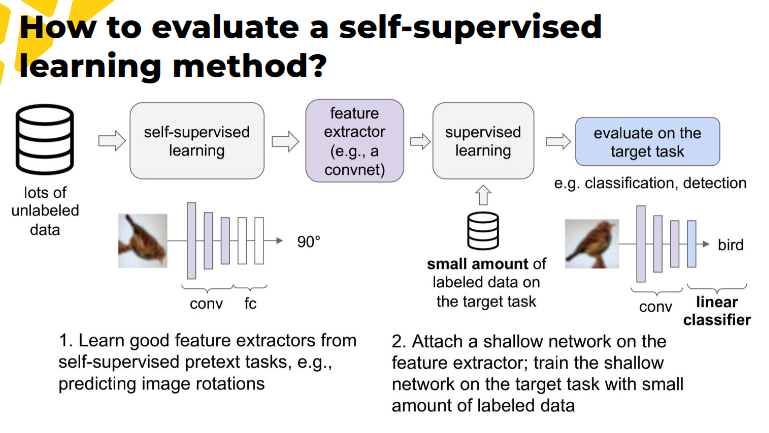
\includegraphics[width=0.9\textwidth]{figures/lecture06_ssl_evaluation_pipeline.png}
    \caption{Оценка self-supervised learning: признаки обучаются на pretext task, затем используются в downstream-задаче.}
\end{figure}

\subsection{Pretext tasks from image transformations}

Ранние self-supervised методы часто строились вокруг image transformations.

Идея: если модель умеет решать задачу, требующую понимания структуры изображения, то она вынуждена выучить полезные visual features.

Примеры:

\begin{itemize}
    \item predict rotations;
    \item predict relative patch locations;
    \item solve jigsaw puzzles;
    \item inpainting;
    \item colorization;
    \item video colorization.
\end{itemize}

\subsection{Pretext task: predict rotations}

В задаче предсказания поворота изображение поворачивается на один из нескольких углов:

\[
0^\circ, 90^\circ, 180^\circ, 270^\circ.
\]

Модель получает повернутое изображение и должна предсказать угол:

\[
y \in \{0,1,2,3\}.
\]

Это обычная задача классификации на 4 класса.

Гипотеза: чтобы определить правильную ориентацию объекта, модель должна иметь некоторый visual commonsense, то есть понимать, как объекты обычно выглядят.

Например, чтобы понять, что птица повернута на \(90^\circ\), модель должна распознавать форму птицы, положение головы, лап, фона и т.д.

% Слайд 13. Pretext task: модель получает изображение, повернутое на 0/90/180/270 градусов, и учится предсказывать класс поворота.
\begin{figure}[H]
    \centering
    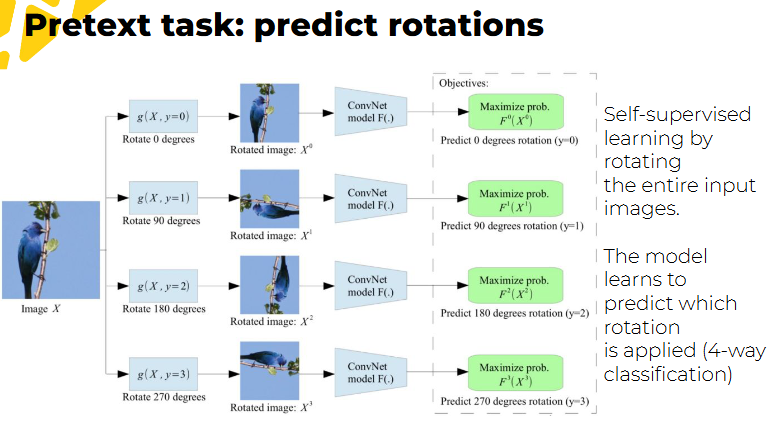
\includegraphics[width=0.9\textwidth]{figures/lecture06_rotation_prediction.png}
    \caption{Self-supervised pretext task: предсказание угла поворота изображения.}
\end{figure}

\subsection{Transfer learned features}

После pretraining на rotation prediction можно проверить, насколько хорошие признаки выучила модель.

Пример evaluation protocol:

\begin{itemize}
    \item self-supervised learning на ImageNet без labels;
    \item затем fine-tuning на Pascal VOC 2007;
    \item оценка classification, detection, segmentation.
\end{itemize}

Такие эксперименты показывают, что даже простая pretext task может дать признаки лучше случайной инициализации.

Но такие признаки всё ещё часто уступают supervised pretraining на ImageNet.

\subsection{Pretext task: predict relative patch locations}

В этой задаче из изображения выбираются два patch-а. Один patch считается центральным, а второй находится в одной из соседних позиций.

Модель должна предсказать относительное положение второго patch-а относительно первого.

Например, label может быть:

\[
y \in \{1,2,\dots,8\},
\]

где 8 классов соответствуют восьми соседним областям вокруг центрального patch-а.

Чтобы решить такую задачу, модель должна понимать spatial structure изображения.

Например, если один patch содержит глаз кота, а другой --- ухо, модель может понять, где ухо обычно расположено относительно глаза.

\subsection{Pretext task: solving jigsaw puzzles}

В jigsaw pretext task изображение разбивается на несколько фрагментов, затем фрагменты перемешиваются.

Модель должна восстановить правильный порядок или предсказать перестановку.

Пусть изображение разбито на \(3 \times 3\) patch-и. Тогда существует много возможных перестановок:

\[
9!
\]

На практике обычно выбирается подмножество перестановок, чтобы задача была вычислительно разумной.

Смысл задачи: модель должна понимать, какие части изображения должны находиться рядом.

% Слайд 18. Jigsaw puzzle pretext task: изображение разбивается на patch-и, они перемешиваются, модель предсказывает правильную перестановку.
\begin{figure}[H]
    \centering
    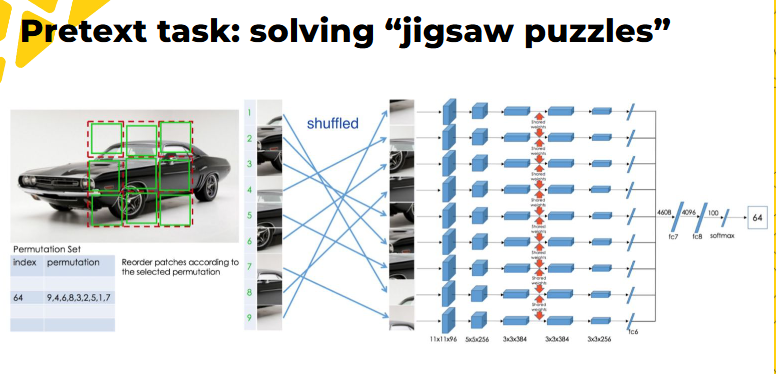
\includegraphics[width=0.9\textwidth]{figures/lecture06_jigsaw_pretext.png}
    \caption{Self-supervised pretext task: решение jigsaw puzzle по patch-ам изображения.}
\end{figure}

\subsection{Pretext task: inpainting}

\textbf{Inpainting} --- задача восстановления отсутствующей части изображения.

Вход:

\[
x_{masked},
\]

где часть изображения закрыта mask-ой.

Модель должна предсказать недостающие пиксели:

\[
\hat{x}_{missing}.
\]

Смысл: чтобы восстановить скрытый фрагмент, модель должна понимать контекст изображения.

Например, если закрыта часть здания, модель должна использовать окна, двери, стены и перспективу вокруг.

% Слайд 21. Inpainting: encoder-decoder архитектура восстанавливает скрытую часть изображения.
\begin{figure}[H]
    \centering
    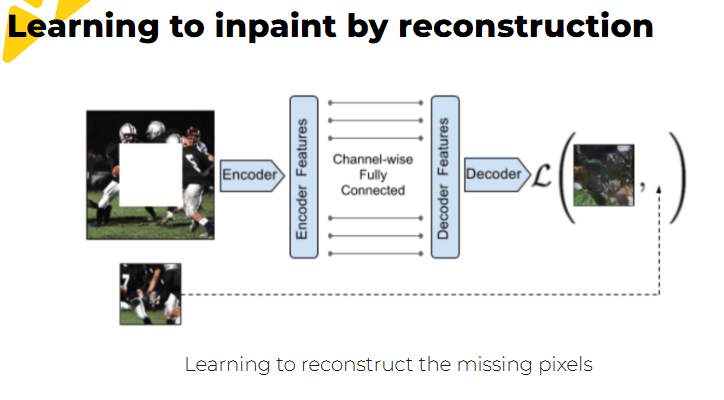
\includegraphics[width=0.85\textwidth]{figures/lecture06_inpainting_encoder_decoder.png}
    \caption{Inpainting: модель восстанавливает скрытую область изображения по контексту.}
\end{figure}

\subsection{Loss для inpainting}

В лекции приводится loss, состоящий из двух частей:

\[
L(x) = L_{recon}(x) + L_{adv}(x).
\]

Здесь:

\begin{itemize}
    \item \(L_{recon}\) --- reconstruction loss;
    \item \(L_{adv}\) --- adversarial loss.
\end{itemize}

Reconstruction loss измеряет близость восстановленного изображения к ground truth:

\[
L_{recon}(x)
=
\left\|
M \odot
\left(
x - F_\theta((1-M)\odot x)
\right)
\right\|_2^2.
\]

Здесь:

\begin{itemize}
    \item \(M\) --- mask скрытой области;
    \item \(1-M\) --- видимая часть изображения;
    \item \(F_\theta\) --- модель восстановления;
    \item \(\odot\) --- поэлементное умножение.
\end{itemize}

Adversarial loss нужен, чтобы восстановленные изображения выглядели более реалистично.

Идея:

\[
L_{adv}
\]

учит модель не просто минимизировать pixel-wise ошибку, а генерировать визуально правдоподобные детали.

\subsection{Pretext task: image coloring}

В colorization исходное изображение переводится в grayscale, а модель должна восстановить цвет.

В цветовом пространстве LAB:

\begin{itemize}
    \item \(L\) channel содержит яркость;
    \item \(a,b\) channels содержат цветовую информацию.
\end{itemize}

Вход:

\[
X \in \mathbb{R}^{H \times W \times 1}
\]

--- grayscale \(L\)-channel.

Выход:

\[
\hat{Y} \in \mathbb{R}^{H \times W \times 2}
\]

--- предсказанные \(a,b\)-channels.

Модель должна восстановить цветовую информацию по структуре изображения.

Это заставляет её понимать объекты: небо обычно голубое, трава зелёная, банан жёлтый и т.д.

\subsection{Split-brain autoencoder}

Split-brain autoencoder строится на идее cross-channel prediction.

Входные каналы изображения делятся на две части:

\[
X_1, X_2.
\]

Одна часть используется для предсказания другой:

\[
F_1(X_1) \rightarrow \hat{X}_2,
\]

\[
F_2(X_2) \rightarrow \hat{X}_1.
\]

Затем признаки из двух ветвей можно объединить.

Идея: модель должна выучить представления, которые связывают разные типы информации об одном и том же объекте.

\subsection{Pretext task: video coloring}

В video colorization используется temporal coherence.

Идея:

\begin{quote}
Если объект движется в видео, его цвет должен быть согласован во времени.
\end{quote}

Модель получает reference frame с цветом и target frame, для которого нужно предсказать цвет.

Она учится устанавливать соответствия между пикселями или регионами reference и target frames в learned feature space.

Предсказанный цвет target pixel можно получить как weighted sum цветов reference frame:

\[
\hat{c}_i
=
\sum_j
\alpha_{ij} c_j^{ref}.
\]

Здесь:

\begin{itemize}
    \item \(\alpha_{ij}\) --- attention-like вес между target pixel \(i\) и reference pixel \(j\);
    \item \(c_j^{ref}\) --- цвет reference pixel.
\end{itemize}

Интересный эффект: tracking может возникать без явной разметки. Если модель научилась переносить цвета между кадрами, она фактически научилась сопоставлять объекты во времени.

\subsection{Проблемы handcrafted pretext tasks}

Pretext tasks на трансформациях изображений полезны, но имеют ограничения:

\begin{itemize}
    \item каждую задачу нужно придумывать вручную;
    \item задача может быть слишком специфичной;
    \item learned representations могут быть привязаны к конкретной pretext task;
    \item признаки не всегда хорошо переносятся на разные downstream-задачи.
\end{itemize}

Это мотивирует более общий подход:

\[
\text{contrastive representation learning}.
\]

\subsection{Contrastive Representation Learning}

\textbf{Contrastive learning} обучает encoder так, чтобы похожие объекты были близко в representation space, а непохожие --- далеко.

Есть:

\begin{itemize}
    \item reference sample \(x\);
    \item positive sample \(x^+\);
    \item negative samples \(x^-_1,\dots,x^-_{N-1}\).
\end{itemize}

Цель:

\[
score(f(x), f(x^+))
\]

должен быть большим, а

\[
score(f(x), f(x^-))
\]

должен быть маленьким.

То есть encoder \(f\) должен давать представления, в которых positive pair близка, а negative pairs далеки.

\subsection{Positive и negative samples}

\textbf{Positive pair} --- два объекта, которые должны считаться похожими.

В vision contrastive learning positive pair часто создаётся через data augmentation одного и того же изображения:

\[
x^+ = t_2(x),
\quad
x = t_1(x),
\]

где \(t_1,t_2\) --- разные случайные augmentations.

Примеры augmentations:

\begin{itemize}
    \item random cropping;
    \item color distortion;
    \item random blur;
    \item horizontal flip.
\end{itemize}

\textbf{Negative samples} --- другие изображения в batch-е или в memory queue.

\subsection{InfoNCE loss}

Пусть есть один positive sample \(x^+\) и \(N-1\) negative samples.

Обозначим score:

\[
s(x, x') = score(f(x), f(x')).
\]

Тогда contrastive loss:

\[
\mathcal{L}
=
-
\log
\frac{
\exp(s(x,x^+))
}{
\exp(s(x,x^+))
+
\sum_{i=1}^{N-1}
\exp(s(x,x_i^-))
}.
\]

Эта функция потерь называется \textbf{InfoNCE loss}.

Её можно понимать как cross entropy loss для \(N\)-way softmax classifier:

\begin{quote}
из \(N\) кандидатов нужно выбрать один positive sample.
\end{quote}

То есть contrastive learning превращается в задачу классификации: найти правильную пару среди неправильных.

InfoNCE также интерпретируется как нижняя оценка mutual information между \(f(x)\) и \(f(x^+)\). Чем больше negative sample size \(N\), тем tighter bound.

\subsection{Cosine similarity}

Часто score function задаётся через cosine similarity:

\[
\operatorname{sim}(u,v)
=
\frac{u^\top v}{\|u\|\|v\|}.
\]

Тогда loss можно записать как:

\[
\mathcal{L}
=
-
\log
\frac{
\exp(\operatorname{sim}(z,z^+)/\tau)
}{
\exp(\operatorname{sim}(z,z^+)/\tau)
+
\sum_{i=1}^{N-1}
\exp(\operatorname{sim}(z,z_i^-)/\tau)
}.
\]

Здесь:

\[
\tau
\]

--- temperature parameter.

Temperature управляет sharpness softmax-а:

\begin{itemize}
    \item маленькая \(\tau\) делает распределение более резким;
    \item большая \(\tau\) делает распределение более сглаженным.
\end{itemize}

\subsection{SimCLR}

\textbf{SimCLR} --- простая и эффективная framework для contrastive learning.

Основные шаги:

\begin{enumerate}
    \item взять изображение \(x\);
    \item применить две случайные augmentations;
    \item получить две views:
    \[
    \tilde{x}_i, \tilde{x}_j;
    \]
    \item пропустить их через encoder \(f\);
    \item получить representations:
    \[
    h_i = f(\tilde{x}_i), \quad h_j = f(\tilde{x}_j);
    \]
    \item пропустить через projection head \(g\):
    \[
    z_i = g(h_i), \quad z_j = g(h_j);
    \]
    \item применить contrastive loss в \(z\)-пространстве.
\end{enumerate}

% Слайд 60. SimCLR: две augmentations одного изображения образуют positive pair.
\begin{figure}[H]
    \centering
    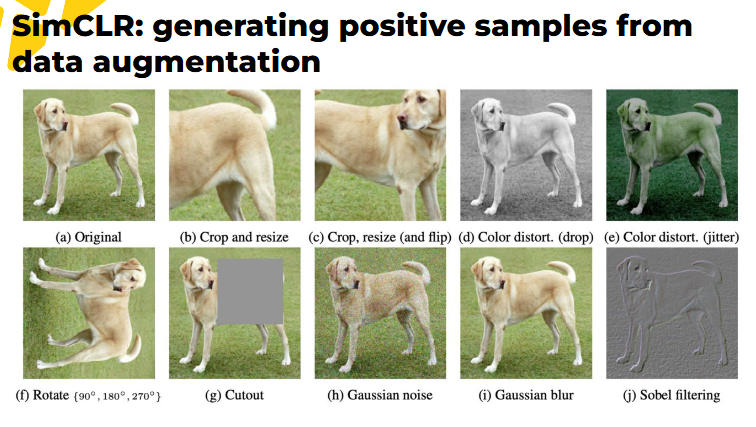
\includegraphics[width=0.9\textwidth]{figures/lecture06_simclr_positive_pairs.png}
    \caption{SimCLR: positive samples создаются как две разные augmentations одного изображения.}
\end{figure}

\subsection{SimCLR loss в mini-batch}

В mini-batch берётся \(N\) исходных изображений. Для каждого создаются две augmentations, поэтому всего получается:

\[
2N
\]

views.

Для каждой view остальные \(2N-1\) views являются кандидатами:

\begin{itemize}
    \item одна из них --- positive pair;
    \item остальные \(2N-2\) --- negatives.
\end{itemize}

Loss считается для каждой из \(2N\) views как reference и затем усредняется.

Особенность SimCLR: все non-positive samples в batch-е используются как negatives.

\subsection{Projection head в SimCLR}

SimCLR использует projection network:

\[
g(\cdot).
\]

Encoder выдаёт:

\[
h = f(x),
\]

projection head выдаёт:

\[
z = g(h).
\]

Contrastive loss применяется к \(z\), но для downstream-задач обычно используется \(h\).

Это важно, потому что contrastive objective может выбрасывать часть информации, полезной для downstream-задач, ради инвариантности к augmentations.

Projection head позволяет:

\begin{itemize}
    \item обучать contrastive пространство \(z\);
    \item сохранить более богатое representation \(h\);
    \item улучшить downstream performance.
\end{itemize}

\subsection{Large batch size в SimCLR}

SimCLR сильно зависит от большого batch size.

Причина: negatives берутся из batch-а. Чем больше batch, тем больше negative samples:

\[
\text{large batch} \Rightarrow \text{many negatives}.
\]

Много negatives делает contrastive task информативнее.

Но большой batch size требует много памяти, особенно при backpropagation. Поэтому в ImageNet экспериментах SimCLR часто требует distributed training на TPU.

\subsection{MoCo}

\textbf{MoCo} расшифровывается как \textbf{Momentum Contrastive Learning}.

Главная проблема SimCLR: чтобы иметь много negatives, нужен большой batch.

MoCo решает это через очередь negative samples.

Основные идеи MoCo:

\begin{itemize}
    \item хранить running queue of keys;
    \item использовать query encoder для текущих примеров;
    \item использовать key encoder для negative samples;
    \item обновлять key encoder медленно через momentum update;
    \item отделить размер mini-batch от числа negatives.
\end{itemize}

% Слайд 72. MoCo: query encoder, key encoder, queue of negative keys и momentum update.
\begin{figure}[H]
    \centering
    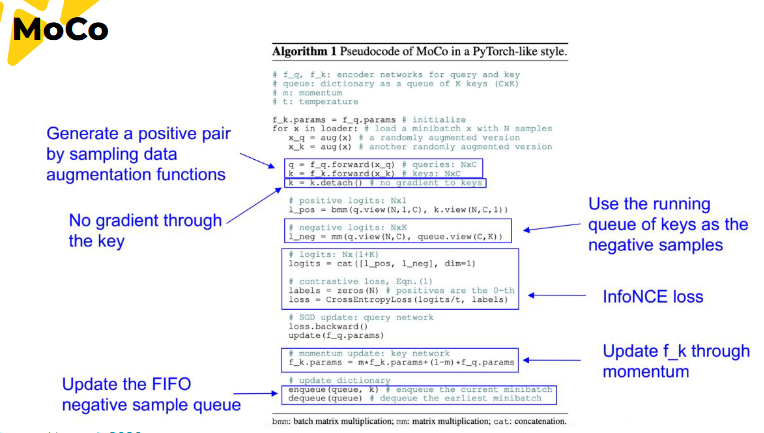
\includegraphics[width=0.9\textwidth]{figures/lecture06_moco_scheme.png}
    \caption{MoCo: очередь negative samples позволяет использовать много negatives без огромного batch size.}
\end{figure}

\subsection{Momentum update в MoCo}

В MoCo есть два encoder-а:

\begin{itemize}
    \item query encoder с параметрами \(\theta_q\);
    \item key encoder с параметрами \(\theta_k\).
\end{itemize}

Query encoder обновляется через backpropagation.

Key encoder обновляется momentum rule:

\[
\theta_k
\leftarrow
m\theta_k + (1-m)\theta_q.
\]

Здесь:

\[
m \in [0,1)
\]

--- momentum coefficient, обычно близкий к 1.

Такой update делает key encoder стабильным, что важно, потому что queue содержит representations, вычисленные на предыдущих шагах.

\subsection{MoCo vs SimCLR}

\begin{table}[H]
\centering
\begin{tabular}{p{0.45\textwidth} p{0.45\textwidth}}
\toprule
\textbf{SimCLR} & \textbf{MoCo} \\
\midrule
Negatives берутся из mini-batch. &
Negatives хранятся в queue. \\

Для большого числа negatives нужен огромный batch. &
Negative sample size отделён от batch size. \\

Требует большой памяти. &
Меньше memory footprint. \\

Простая end-to-end схема. &
Есть momentum key encoder. \\

Сильно выигрывает от projection head и strong augmentation. &
MoCo v2 также использует projection head и strong augmentation. \\
\bottomrule
\end{tabular}
\caption{Сравнение SimCLR и MoCo.}
\end{table}

\subsection{MoCo v2}

MoCo v2 объединяет идеи SimCLR и MoCo:

\begin{itemize}
    \item от SimCLR:
    \begin{itemize}
        \item non-linear projection head;
        \item strong data augmentation;
    \end{itemize}

    \item от MoCo:
    \begin{itemize}
        \item momentum-updated queue;
        \item большое число negatives без огромного batch size.
    \end{itemize}
\end{itemize}

Главный вывод из сравнения:

\begin{itemize}
    \item non-linear projection head важен;
    \item strong augmentation важна;
    \item decoupling mini-batch size и negative sample size позволяет MoCo v2 быть эффективным при меньшем batch size.
\end{itemize}

\subsection{Instance vs sequence contrastive learning}

SimCLR и MoCo --- примеры \textbf{instance contrastive learning}.

В них positive pair обычно создаётся из одного объекта через augmentation.

Но contrastive learning можно применять и к последовательностям.

Пример:

\[
\text{Contrastive Predictive Coding, CPC}.
\]

\subsection{Contrastive Predictive Coding}

\textbf{CPC} расшифровывается как:

\[
\text{Contrastive Predictive Coding}.
\]

Название отражает три идеи:

\begin{itemize}
    \item \textbf{Contrastive}: модель различает правильные и неправильные future samples.
    \item \textbf{Predictive}: модель предсказывает будущие паттерны по текущему контексту.
    \item \textbf{Coding}: модель учит полезные feature vectors, или codes.
\end{itemize}

% Слайд 78. CPC: contrastive, predictive, coding — различение правильных и неправильных будущих последовательностей.
\begin{figure}[H]
    \centering
    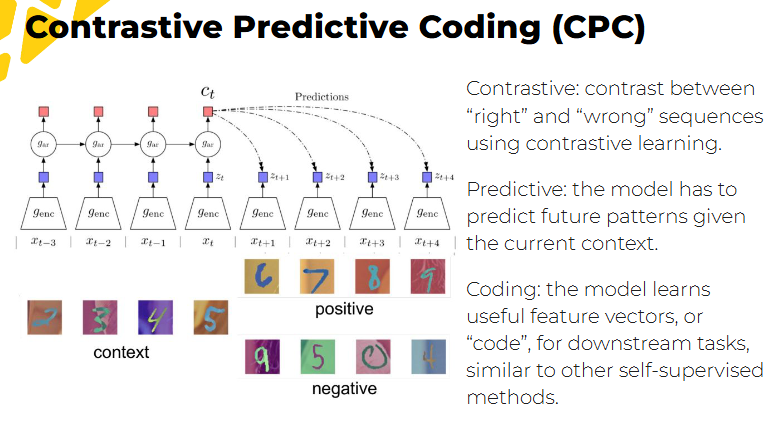
\includegraphics[width=0.9\textwidth]{figures/lecture06_cpc_overview.png}
    \caption{Contrastive Predictive Coding: модель учится отличать правильное будущее от неправильного.}
\end{figure}

\subsection{CPC pipeline}

CPC работает с последовательностью:

\[
x_1, x_2, \dots, x_T.
\]

\subsubsection{Шаг 1: encode samples}

Каждый элемент последовательности кодируется encoder-ом:

\[
z_t = g_{enc}(x_t).
\]

\subsubsection{Шаг 2: summarize context}

Контекст до момента \(t\) агрегируется autoregressive model:

\[
c_t = g_{ar}(z_{\leq t}).
\]

В оригинальной статье используется GRU-RNN.

\subsubsection{Шаг 3: contrastive prediction}

Модель пытается предсказать future code:

\[
z_{t+k}
\]

по context code:

\[
c_t.
\]

Score function зависит от горизонта \(k\):

\[
score_k(c_t, z_{t+k})
=
z_{t+k}^{\top} W_k c_t.
\]

Здесь \(W_k\) --- обучаемая матрица для шага \(k\).

Затем применяется InfoNCE loss: правильный future sample должен иметь высокий score, неправильные future samples --- низкий.

\subsection{Применения CPC}

CPC можно применять к разным типам последовательностей:

\begin{itemize}
    \item audio;
    \item изображения как последовательность patch-ей;
    \item видео;
    \item текст;
    \item временные ряды.
\end{itemize}

Для изображений можно разбить картинку на patch-и и рассматривать строки patch-ей сверху вниз как последовательность.

Тогда верхняя часть изображения является context, а нижнюю нужно предсказать contrastive образом.

\subsection{Contrastive learning и mutual information}

InfoNCE можно рассматривать как способ максимизировать нижнюю оценку mutual information между представлениями positive pair.

Интуитивно:

\[
I(f(x); f(x^+))
\]

должна быть большой.

То есть representation reference sample должно содержать информацию о representation positive sample.

Чем больше negative samples, тем сложнее задача и тем tighter bound на mutual information.

\subsection{Другие примеры contrastive/self-supervised learning}

В лекции также упоминаются современные и смежные методы:

\begin{itemize}
    \item MoCo v3;
    \item Masked Autoencoders;
    \item CLIP;
    \item Dense Object Net;
    \item DINO;
    \item DINO v2.
\end{itemize}

Особенно важный пример --- \textbf{CLIP}.

CLIP использует contrastive learning между изображениями и текстовыми описаниями.

Positive pair:

\[
(\text{image}, \text{matching caption}).
\]

Negative pairs:

\[
(\text{image}, \text{wrong captions}).
\]

Модель учит общее image-text representation space.

\subsection{Главные выводы}

\begin{itemize}
    \item Self-supervised learning позволяет учиться без ручной разметки.
    \item Pretext task создаётся автоматически и используется для обучения хороших признаков.
    \item Качество pretext task не так важно, как качество learned representations на downstream tasks.
    \item Image transformation pretext tasks включают rotation prediction, jigsaw, inpainting и colorization.
    \item Handcrafted pretext tasks могут быть слишком специфичными.
    \item Contrastive learning предлагает более общий принцип: positive pairs должны быть близко, negative pairs далеко.
    \item InfoNCE loss можно понимать как cross entropy для выбора positive sample среди \(N\) кандидатов.
    \item SimCLR создаёт positive pairs через data augmentation и использует negatives из batch-а.
    \item Projection head в SimCLR помогает сохранить полезную информацию в encoder representation.
    \item MoCo использует queue negatives и momentum encoder, чтобы не требовать огромный batch.
    \item CPC применяет contrastive learning к последовательностям и учится предсказывать будущее.
\end{itemize}

\subsection{Что важно помнить к экзамену}

\begin{enumerate}
    \item Определение self-supervised learning:
    labels для pretext task генерируются автоматически.

    \item Что pretext task нужна не сама по себе, а для обучения feature extractor.

    \item Как оценивают self-supervised метод:
    \[
    \text{pretext training}
    \rightarrow
    \text{feature extractor}
    \rightarrow
    \text{downstream task}.
    \]

    \item Примеры pretext tasks:
    \begin{itemize}
        \item rotation prediction;
        \item relative patch location;
        \item jigsaw puzzle;
        \item inpainting;
        \item colorization.
    \end{itemize}

    \item Общая идея contrastive learning:
    \[
    score(f(x),f(x^+)) \text{ высокий},
    \]
    \[
    score(f(x),f(x^-)) \text{ низкий}.
    \]

    \item InfoNCE loss:
    \[
    \mathcal{L}
    =
    -
    \log
    \frac{
    \exp(s(x,x^+))
    }{
    \exp(s(x,x^+))
    +
    \sum_{i=1}^{N-1}
    \exp(s(x,x_i^-))
    }.
    \]

    \item Cosine similarity:
    \[
    \operatorname{sim}(u,v)
    =
    \frac{u^\top v}{\|u\|\|v\|}.
    \]

    \item Temperature-scaled loss:
    \[
    \mathcal{L}
    =
    -
    \log
    \frac{
    \exp(\operatorname{sim}(z,z^+)/\tau)
    }{
    \exp(\operatorname{sim}(z,z^+)/\tau)
    +
    \sum_i
    \exp(\operatorname{sim}(z,z_i^-)/\tau)
    }.
    \]

    \item SimCLR:
    \begin{itemize}
        \item positive pair = две augmentations одного изображения;
        \item negatives = остальные samples в batch;
        \item используется projection head \(g(\cdot)\);
        \item нужен большой batch size.
    \end{itemize}

    \item MoCo:
    \begin{itemize}
        \item использует queue negative keys;
        \item использует momentum key encoder;
        \item decouples batch size and number of negatives.
    \end{itemize}

    \item Momentum update:
    \[
    \theta_k
    \leftarrow
    m\theta_k + (1-m)\theta_q.
    \]

    \item CPC:
    \[
    z_t = g_{enc}(x_t),
    \]
    \[
    c_t = g_{ar}(z_{\leq t}),
    \]
    \[
    score_k(c_t,z_{t+k})
    =
    z_{t+k}^{\top}W_kc_t.
    \]

    \item Отличие instance contrastive learning от sequence contrastive learning:
    \begin{itemize}
        \item instance-level: сравниваются views одного объекта;
        \item sequence-level: правильное будущее сравнивается с неправильным.
    \end{itemize}
\end{enumerate}
```
```latex
\section{Лекция 7. Introduction to Reinforcement Learning}

\subsection{План лекции}

В этой лекции рассматриваются:

\begin{itemize}
    \item постановка задачи Reinforcement Learning;
    \item отличие RL от supervised и unsupervised learning;
    \item агент, среда, действие, состояние, награда;
    \item multi-armed bandits как простая RL-постановка;
    \item MDP formalism;
    \item связь RL с психологией;
    \item cross-entropy method;
    \item табличный и приближённый cross-entropy method;
    \item базовые определения value functions и Q-functions;
    \item переход от табличных методов к аппроксимации функций.
\end{itemize}

Главная идея лекции: Reinforcement Learning изучает обучение агента через взаимодействие со средой. В отличие от supervised learning, у агента обычно нет правильных ответов для каждого состояния; он получает только feedback в виде reward и должен научиться стратегии, максимизирующей долгосрочную суммарную награду.

\subsection{Supervised Learning и Reinforcement Learning}

В supervised learning есть обучающая выборка:

\[
(x_i, y_i),
\]

где:

\begin{itemize}
    \item \(x_i \in \mathcal{X}\) --- объект;
    \item \(y_i \in \mathcal{Y}\) --- правильный ответ;
    \item \(L(\hat{y}, y)\) --- loss function;
    \item \(f \in \mathcal{F}\) --- модель из некоторого семейства.
\end{itemize}

Цель supervised learning:

\[
f^*
=
\arg\min_f
L(f(x), y).
\]

Обычно предполагается, что объекты выборки независимы и одинаково распределены, то есть i.i.d. Также loss часто дифференцируем, что позволяет использовать gradient-based optimization.

В Reinforcement Learning ситуация другая.

Обычно:

\begin{itemize}
    \item нет reference answers;
    \item непонятно, какое действие правильно в каждом конкретном состоянии;
    \item loss часто трудно явно сформулировать;
    \item действия агента влияют на будущие наблюдения;
    \item качество действия может проявиться не сразу, а через много шагов.
\end{itemize}

Например, если мы хотим научить робота ходить, у нас нет правильного действия для каждого состояния суставов. Мы можем только задать reward: например, робот получает награду за продвижение вперёд и штраф за падение.

\subsection{Базовая схема Reinforcement Learning}

В RL есть две основные сущности:

\begin{itemize}
    \item \textbf{agent} --- обучаемая система;
    \item \textbf{environment} --- среда, с которой агент взаимодействует.
\end{itemize}

На каждом шаге:

\begin{enumerate}
    \item среда выдаёт агенту observation или state;
    \item агент выбирает action;
    \item действие влияет на среду;
    \item среда возвращает reward и новое observation/state.
\end{enumerate}

Схема:

\[
s_t
\rightarrow
a_t
\rightarrow
r_t, s_{t+1}.
\]

Здесь:

\begin{itemize}
    \item \(s_t\) --- state или observation в момент \(t\);
    \item \(a_t\) --- action агента;
    \item \(r_t\) --- reward;
    \item \(s_{t+1}\) --- следующее состояние.
\end{itemize}

% Слайд 10. Общая схема agent-environment loop: observation -> agent -> action -> environment -> feedback.
\begin{figure}[H]
    \centering
    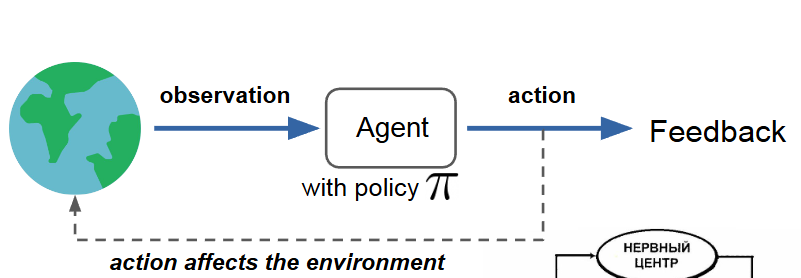
\includegraphics[width=0.85\textwidth]{figures/lecture07_agent_environment_loop.png}
    \caption{Основной цикл Reinforcement Learning: агент наблюдает состояние, выбирает действие и получает feedback от среды.}
\end{figure}

\subsection{Policy}

\textbf{Policy} --- стратегия поведения агента.

Policy задаёт, какое действие агент выбирает в данном состоянии.

Детерминированная policy:

\[
\pi(s) = a.
\]

Стохастическая policy:

\[
\pi(a \mid s)
=
P(\text{take action } a \text{ in state } s).
\]

В стохастическом случае policy задаёт распределение вероятностей по действиям.

Например, если в состоянии \(s\) доступно три действия:

\[
a_1, a_2, a_3,
\]

то policy может быть:

\[
\pi(a_1 \mid s)=0.2,
\quad
\pi(a_2 \mid s)=0.5,
\quad
\pi(a_3 \mid s)=0.3.
\]

\subsection{Примеры RL-задач}

\subsubsection{Управление роботом}

Для робота:

\begin{itemize}
    \item observation --- данные с датчиков, изображение, положение суставов;
    \item action --- управляющие сигналы моторам;
    \item reward --- скорость движения, устойчивость, штраф за падение.
\end{itemize}

\subsubsection{Управление вертолётом}

Для вертолёта:

\begin{itemize}
    \item observation --- accelerometer, gyroscope, engine data;
    \item action --- изменение скорости вращения, угла и других управляющих параметров;
    \item reward --- мера качества полёта.
\end{itemize}

\subsubsection{Видеоигры}

Для Atari или DOOM:

\begin{itemize}
    \item observation --- изображение или последовательность кадров;
    \item action --- move, fire, turn и т.д.;
    \item reward --- score, health, progress.
\end{itemize}

\subsection{Ключевые вопросы Reinforcement Learning}

В RL сразу возникают важные вопросы.

\subsubsection{Что такое оптимальное действие?}

Можно пытаться максимизировать reward на следующем шаге:

\[
\max r_t.
\]

Но иногда действие, которое хорошо прямо сейчас, плохо в долгосрочной перспективе.

Поэтому обычно цель RL --- максимизировать долгосрочную суммарную награду:

\[
\sum_t r_t.
\]

\subsubsection{Explore or exploit?}

Агент должен выбирать между:

\begin{itemize}
    \item \textbf{exploitation} --- использовать уже известную хорошую стратегию;
    \item \textbf{exploration} --- пробовать новые действия, чтобы найти потенциально лучшую стратегию.
\end{itemize}

Проблема:

\begin{itemize}
    \item если всегда exploit, агент может никогда не найти лучшую стратегию;
    \item если слишком много explore, агент теряет reward на плохих действиях.
\end{itemize}

Это называется exploration-exploitation tradeoff.

\subsection{Multi-Armed Bandits}

Multi-armed bandit --- одна из простейших RL-постановок.

Есть несколько действий, или ``ручек автомата'':

\[
a \in \{1,2,\dots,K\}.
\]

На каждом шаге агент выбирает одно действие и получает reward.

Особенность bandit setting:

\begin{itemize}
    \item обычно нет сложного состояния;
    \item действие не меняет состояние среды в сложном смысле;
    \item главная задача --- понять, какое действие даёт наибольшую ожидаемую награду.
\end{itemize}

Цель:

\[
a^*
=
\arg\max_a
\mathbb{E}[r \mid a].
\]

Bandits хорошо иллюстрируют exploration-exploitation tradeoff: нужно пробовать разные действия, но постепенно выбирать лучшие.

\subsection{MDP formalism}

Более общая постановка RL описывается через Markov Decision Process, или MDP.

MDP задаётся набором:

\[
(\mathcal{S}, \mathcal{A}, P, R).
\]

Где:

\begin{itemize}
    \item \(\mathcal{S}\) --- множество состояний;
    \item \(\mathcal{A}\) --- множество действий;
    \item \(P(s_{t+1} \mid s_t, a_t)\) --- dynamics или transition probability;
    \item \(R\) --- reward function.
\end{itemize}

В лекции используются обозначения:

\[
s \in \mathcal{S},
\]

\[
a \in \mathcal{A},
\]

\[
r \in \mathbb{R}.
\]

Динамика среды:

\[
P(s_{t+1} \mid s_t, a_t).
\]

% Слайд 16. MDP formalism: state, action, reward, dynamics и Markov property.
\begin{figure}[H]
    \centering
    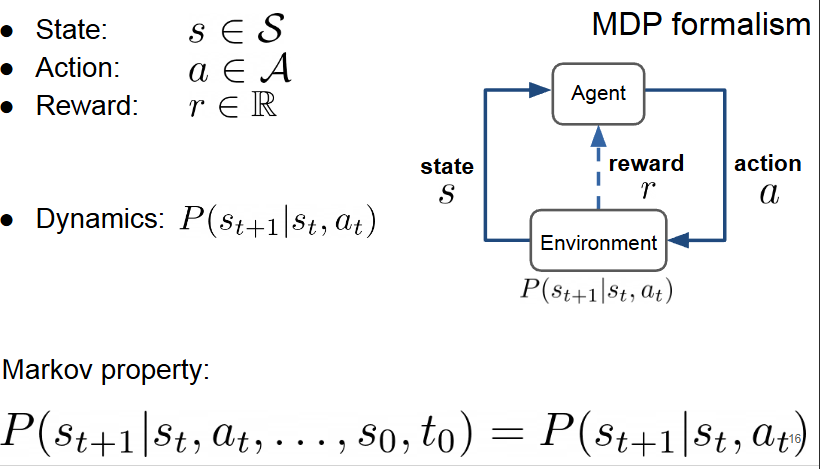
\includegraphics[width=0.85\textwidth]{figures/lecture07_mdp_formalism.png}
    \caption{MDP formalism: агент выбирает действие в состоянии, среда возвращает reward и следующее состояние.}
\end{figure}

\subsection{Markov property}

Ключевое свойство MDP --- Markov property.

Оно означает, что будущее зависит от прошлого только через текущее состояние и текущее действие:

\[
P(s_{t+1} \mid s_t, a_t, \dots, s_0, a_0)
=
P(s_{t+1} \mid s_t, a_t).
\]

Иными словами, если мы знаем \(s_t\) и \(a_t\), то вся предыдущая история уже не нужна для предсказания \(s_{t+1}\).

Это сильное предположение. На практике observation может не содержать всей информации о состоянии. Тогда возникает частично наблюдаемая задача, и агенту может понадобиться память.

\subsection{Total reward}

Суммарная награда за session или episode:

\[
R =
\sum_t r_t.
\]

Если используется discount factor \(\gamma\), то discounted return:

\[
G_t =
\sum_{t'=t}^{T}
\gamma^{t'-t} r_{t'}.
\]

Здесь:

\[
\gamma \in [0,1].
\]

Смысл \(\gamma\):

\begin{itemize}
    \item если \(\gamma\) близко к 0, агент фокусируется на ближайшей награде;
    \item если \(\gamma\) близко к 1, агент учитывает дальнее будущее.
\end{itemize}

Цель RL:

\[
\pi^*
=
\arg\max_\pi
\mathbb{E}_{\pi}[R].
\]

То есть нужно найти policy, максимизирующую expected cumulative reward.

\subsection{Value function и Q-function}

\textbf{Value function} показывает, насколько хорошо находиться в состоянии \(s\), если дальше следовать policy \(\pi\):

\[
V^\pi(s)
=
\mathbb{E}_{\pi}
[
G_t \mid s_t=s
].
\]

\textbf{Q-function} показывает, насколько хорошо выполнить действие \(a\) в состоянии \(s\), а затем следовать policy \(\pi\):

\[
Q^\pi(s,a)
=
\mathbb{E}_{\pi}
[
G_t \mid s_t=s, a_t=a
].
\]

Эти функции важны, потому что позволяют оценивать не только immediate reward, но и будущие последствия действий.

\subsection{Bellman relations}

Для value и Q-functions можно записать рекуррентные соотношения.

Для Q-function:

\[
Q^\pi(s,a)
=
\mathbb{E}_{s'}
[
r_t + \gamma V^\pi(s_{t+1})
].
\]

Также:

\[
Q^\pi(s,a)
=
\mathbb{E}_{s',a'\sim\pi}
[
r_t + \gamma Q^\pi(s_{t+1},a_{t+1})
].
\]

Оптимальная Q-function:

\[
Q^*(s,a)
\]

не хуже любой другой policy:

\[
Q^*(s,a) \geq Q^\pi(s,a)
\]

для всех \(\pi, s, a\).

Оптимальная policy:

\[
\pi^*(s)
=
\arg\max_a Q^*(s,a).
\]

Bellman optimality equation:

\[
Q^*(s_t,a)
=
\mathbb{E}_{s_{t+1}}
\left[
r_t +
\gamma \max_{a'} Q^*(s_{t+1},a')
\right].
\]

\subsection{Связь RL с психологией}

В лекции упоминаются психологические аналогии:

\begin{itemize}
    \item classical conditioning;
    \item operant conditioning;
    \item Thorndike experiment;
    \item Skinner box.
\end{itemize}

Идея operant conditioning: поведение может усиливаться или ослабляться в зависимости от последствий.

Например, если крыса нажимает рычаг и получает еду, вероятность такого поведения растёт. Это похоже на RL: действие, приведшее к положительному reward, становится более вероятным.

\subsection{Как максимизировать reward}

Общая идея policy optimization:

\begin{enumerate}
    \item сыграть несколько sessions с текущей policy;
    \item получить rewards;
    \item обновить policy на основе feedback;
    \item повторить.
\end{enumerate}

То есть обучение происходит через trial and error:

\[
\pi_0
\rightarrow
\text{episodes}
\rightarrow
\text{rewards}
\rightarrow
\pi_1
\rightarrow
\dots
\]

\subsection{Cross-Entropy Method}

\textbf{Cross-Entropy Method, CEM} --- простой policy search метод.

Идея:

\begin{itemize}
    \item сгенерировать много episodes;
    \item выбрать лучшие episodes, называемые elite sessions;
    \item обновить policy так, чтобы она чаще повторяла действия из elite sessions;
    \item повторять процесс.
\end{itemize}

CEM не требует дифференцируемой среды и может использоваться как простой baseline для RL.

\subsection{Cross-Entropy Method: tabular case}

В табличном случае policy можно представить матрицей:

\[
\pi(a \mid s) = A_{s,a}.
\]

Каждая строка соответствует состоянию, каждый столбец --- действию.

Для каждого состояния:

\[
\sum_a A_{s,a}=1.
\]

Алгоритм:

\begin{enumerate}
    \item инициализировать policy matrix \(A\);
    \item сэмплировать \(N\) sessions;
    \item выбрать \(M\) elite sessions с наибольшими rewards;
    \item обновить policy по state-action pairs из elite sessions;
    \item повторить.
\end{enumerate}

% Слайд 23. Cross-entropy method в tabular case: случайная policy matrix постепенно превращается в настроенную policy.
\begin{figure}[H]
    \centering
    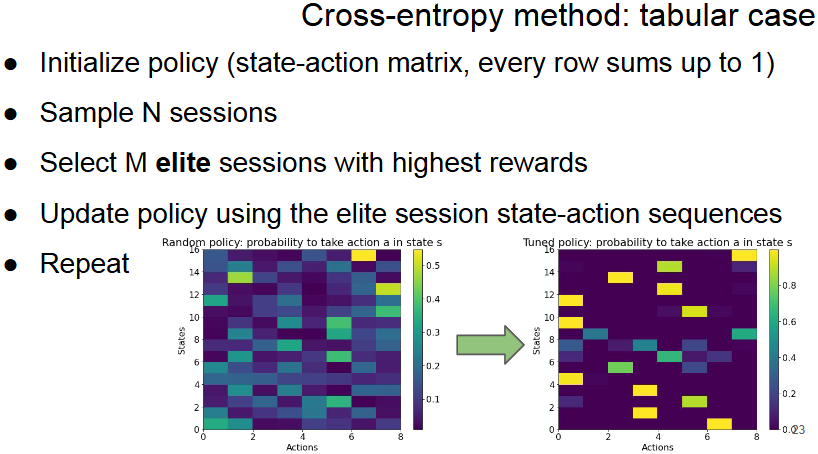
\includegraphics[width=0.85\textwidth]{figures/lecture07_cem_tabular_overview.png}
    \caption{Cross-Entropy Method в табличном случае: policy matrix обновляется по elite sessions.}
\end{figure}

\subsection{Обновление policy в tabular CEM}

Пусть elite sessions содержат пары:

\[
(s_0,a_0), (s_1,a_1), \dots.
\]

Новая policy оценивается как частота выбора действия \(a\) в состоянии \(s\) среди elite sessions:

\[
\pi_{\text{new}}(a \mid s)
=
\frac{
\sum_{(s_t,a_t)\in Elite}
\mathbb{I}[s_t=s]\mathbb{I}[a_t=a]
}{
\sum_{(s_t,a_t)\in Elite}
\mathbb{I}[s_t=s]
}.
\]

Иными словами:

\[
\pi_{\text{new}}(a \mid s)
=
\frac{
\text{how many times took action } a \text{ at state } s
}{
\text{how many times was at state } s
}.
\]

% Слайд 36. Обновление policy в tabular CEM как частота action среди elite sessions.
\begin{figure}[H]
    \centering
    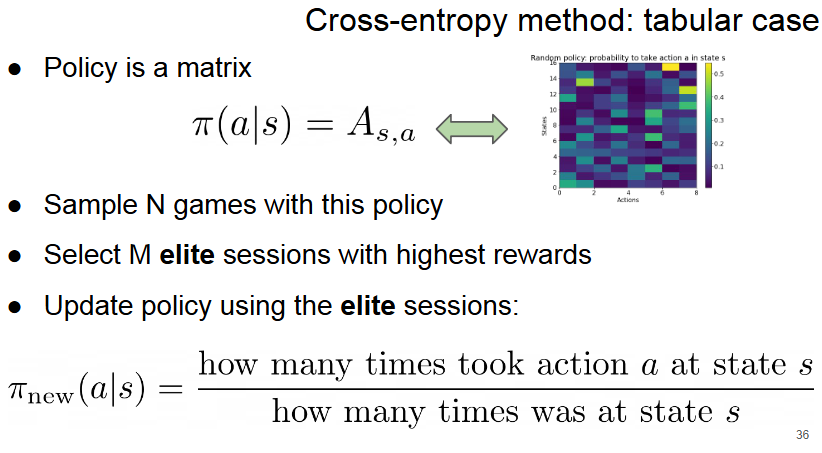
\includegraphics[width=0.85\textwidth]{figures/lecture07_cem_policy_update.png}
    \caption{Обновление tabular policy: вероятность действия равна его частоте среди elite sessions.}
\end{figure}

\subsection{Проблема больших пространств состояний}

Tabular policy работает только если число состояний и действий небольшое.

В реальных задачах пространство состояний может быть огромным или бесконечным.

Например, если observation --- изображение из игры, то число возможных состояний гигантское:

\[
|\mathcal{S}| \approx 2^{210\cdot 160\cdot 8\cdot 3}.
\]

Хранить таблицу для всех состояний невозможно.

Поэтому нужно переходить от таблиц к функциям:

\[
\pi(a \mid s) = f_\theta(s,a)
\]

или

\[
Q(s,a) \approx Q_\theta(s,a).
\]

\subsection{Approximate Cross-Entropy Method}

В approximate CEM policy задаётся не таблицей, а параметрической моделью.

Например:

\[
\pi(a \mid s) = f_\theta(a,s).
\]

Модель получает state и выдаёт вероятности действий.

Это может быть:

\begin{itemize}
    \item logistic regression;
    \item random forest classifier;
    \item neural network;
    \item другая модель классификации.
\end{itemize}

Алгоритм:

\begin{enumerate}
    \item сэмплировать \(N\) sessions с текущей policy;
    \item выбрать \(M\) elite sessions;
    \item собрать training set:
    \[
    \text{states} \rightarrow \text{actions};
    \]
    \item обучить модель предсказывать elite actions по elite states.
\end{enumerate}

То есть в кодовой форме:

\[
\texttt{model.fit(elite\_states, elite\_actions)}.
\]

Функция потерь:

\[
\pi_{\text{new}}
=
\arg\max_\pi
\sum_{(s_t,a_t)\in Elite}
\log \pi(a_t \mid s_t).
\]

% Слайд 38. Approximate CEM: policy задаётся моделью, которая обучается на elite states и elite actions.
\begin{figure}[H]
    \centering
    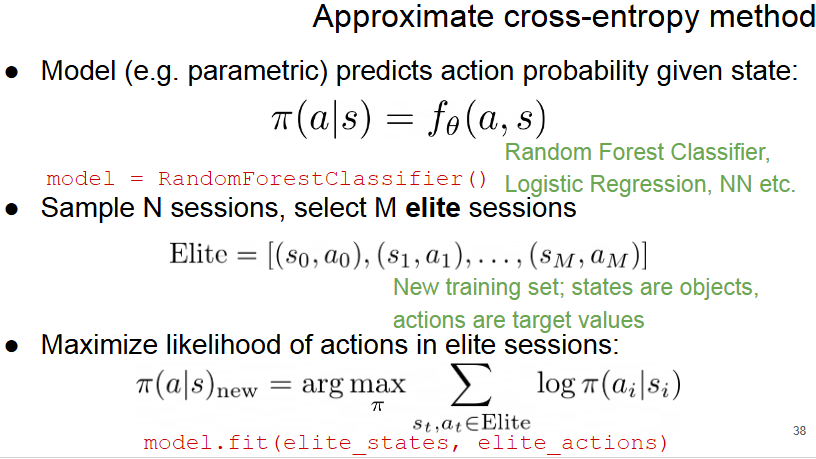
\includegraphics[width=0.9\textwidth]{figures/lecture07_approximate_cem.png}
    \caption{Approximate Cross-Entropy Method: elite states становятся объектами, elite actions --- target values.}
\end{figure}

\subsection{Continuous action space}

Если action space непрерывное, policy может задавать распределение над действиями.

Например, нормальное распределение:

\[
\pi(a \mid s)
=
\mathcal{N}
\left(
\mu_\theta(s),
\sigma_\gamma(s)
\right).
\]

Здесь:

\begin{itemize}
    \item \(\mu_\theta(s)\) --- среднее действия;
    \item \(\sigma_\gamma(s)\) --- стандартное отклонение;
    \item оба параметра могут предсказываться моделями.
\end{itemize}

В простом случае \(\sigma\) можно считать константой, а модель обучает только среднее действие.

Тогда approximate CEM становится похож на regression:

\[
s \mapsto a.
\]

\subsection{Useful ideas для CEM}

В лекции перечислены практические идеи:

\begin{itemize}
    \item использовать elite sessions из нескольких прошлых итераций;
    \item регуляризовать policy через entropy;
    \item сэмплировать sessions параллельно;
    \item использовать память агента, например RNN.
\end{itemize}

\subsubsection{Использование прошлых elite sessions}

Если использовать elite sessions за последние 3--5 итераций, опыт прошлых итераций сохраняется.

Плюс:

\begin{itemize}
    \item меньше забывания полезного поведения.
\end{itemize}

Минус:

\begin{itemize}
    \item сходимость может быть медленнее на простых средах.
\end{itemize}

\subsubsection{Entropy regularization}

Низкая entropy policy означает слабую exploration.

Если policy слишком быстро становится почти детерминированной, агент может перестать исследовать альтернативные действия.

Entropy regularization помогает сохранять разнообразие действий:

\[
H(\pi(\cdot \mid s))
=
-
\sum_a
\pi(a \mid s)\log \pi(a \mid s).
\]

Чем выше entropy, тем более случайна policy.

\subsection{Q-learning}

В конце презентации вводится Q-learning.

Q-learning пытается выучить оптимальную Q-function:

\[
Q^*(s,a).
\]

Обновление Q-learning:

\[
Q(s_t,a_t)
\leftarrow
Q(s_t,a_t)
+
\alpha
\left[
r_t
+
\gamma \max_{a'} Q(s_{t+1},a')
-
Q(s_t,a_t)
\right].
\]

Здесь:

\begin{itemize}
    \item \(\alpha\) --- learning rate;
    \item \(\gamma\) --- discount factor;
    \item выражение в квадратных скобках --- temporal difference error.
\end{itemize}

Temporal difference error:

\[
\delta_t
=
r_t
+
\gamma \max_{a'}Q(s_{t+1},a')
-
Q(s_t,a_t).
\]

\subsection{Q-learning как MSE minimization}

Q-learning можно рассматривать как минимизацию ошибки между текущим \(Q(s_t,a_t)\) и target:

\[
y_t =
r_t + \gamma \max_{a'}Q(s_{t+1},a').
\]

Loss:

\[
L
=
\left(
r_t
+
\gamma \max_{a'}Q(s_{t+1},a')
-
Q(s_t,a_t)
\right)^2.
\]

Важно: target часто рассматривается как константа относительно текущего gradient step. Это нужно для стабильности обучения.

\subsection{Approximate Q-learning}

Когда state space большой, таблицу \(Q(s,a)\) хранить нельзя.

Тогда Q-function аппроксимируется моделью:

\[
Q_\theta(s,a).
\]

Например, нейронной сетью.

Переход:

\[
\text{before: remember } Q(s,a) \text{ for all states and actions},
\]

\[
\text{now: approximate } Q(s,a) \text{ with a function}.
\]

Objective:

\[
\arg\min_\theta
\left(
Q_\theta(s_t,a_t)
-
\left[
r_t + \gamma \max_{a'}Q_\theta(s_{t+1},a')
\right]
\right)^2.
\]

Для изображений можно использовать CNN, которая принимает кадр игры и выдаёт Q-values для всех действий.

\subsection{Basic Deep Q-Learning}

В Deep Q-Learning Q-function задаётся нейронной сетью.

Для Atari-подобных задач:

\begin{itemize}
    \item вход --- изображение или stack кадров;
    \item несколько convolutional layers извлекают visual features;
    \item dense layers формируют представление;
    \item выход --- Q-values для всех actions.
\end{itemize}

Если действий \(K\), то сеть выдаёт:

\[
Q(s,a_1), Q(s,a_2), \dots, Q(s,a_K).
\]

Действие выбирается как:

\[
a^*
=
\arg\max_a Q(s,a).
\]

\subsection{RL vs Supervised Learning}

\begin{table}[H]
\centering
\begin{tabular}{p{0.45\textwidth} p{0.45\textwidth}}
\toprule
\textbf{Supervised Learning} & \textbf{Reinforcement Learning} \\
\midrule
Учится приближать reference answers. &
Учится оптимальной стратегии через trial and error. \\

Нужны правильные ответы \(y\). &
Нужен feedback на действия агента. \\

Модель не влияет на входные данные. &
Действия агента влияют на среду и будущие наблюдения. \\

Обычно есть фиксированный dataset. &
Данные зависят от текущей policy. \\

Цель обычно локальная: минимизировать loss на примерах. &
Цель долгосрочная: максимизировать cumulative reward. \\
\bottomrule
\end{tabular}
\caption{Сравнение supervised learning и reinforcement learning.}
\end{table}

\subsection{RL vs Unsupervised Learning}

\begin{table}[H]
\centering
\begin{tabular}{p{0.45\textwidth} p{0.45\textwidth}}
\toprule
\textbf{Unsupervised Learning} & \textbf{Reinforcement Learning} \\
\midrule
Изучает структуру данных. &
Учится оптимальной стратегии через взаимодействие. \\

Feedback не требуется. &
Нужен reward или другой feedback. \\

Модель не влияет на данные. &
Действия агента меняют будущие состояния. \\

Обычно нет понятия действия. &
Action является центральным объектом. \\

Цель --- representation, clustering, density и т.д. &
Цель --- maximize expected cumulative reward. \\
\bottomrule
\end{tabular}
\caption{Сравнение unsupervised learning и reinforcement learning.}
\end{table}

\subsection{Reward formulation}

Формулировка reward сильно влияет на поведение агента.

Если reward задан плохо, агент может научиться нежелательному поведению.

Например:

\begin{itemize}
    \item если награждать робота только за скорость, он может падать, но двигаться быстро;
    \item если награждать игрового агента только за очки, он может эксплуатировать баги среды;
    \item если штрафовать слишком сильно, агент может выбрать бездействие.
\end{itemize}

Поэтому reward design --- одна из центральных практических проблем RL.

\subsection{Главные выводы}

\begin{itemize}
    \item Reinforcement Learning отличается от supervised learning отсутствием правильных ответов для каждого состояния.
    \item Агент учится через взаимодействие со средой и feedback в виде reward.
    \item Policy задаёт стратегию выбора действий:
    \[
    \pi(a \mid s).
    \]

    \item Цель RL --- максимизировать expected cumulative reward:
    \[
    \pi^*
    =
    \arg\max_\pi
    \mathbb{E}_\pi[R].
    \]

    \item MDP формализует RL через states, actions, rewards и transition dynamics.
    \item Markov property означает, что будущее зависит только от текущего состояния и действия.
    \item Exploration-exploitation tradeoff --- фундаментальная проблема RL.
    \item Cross-Entropy Method обновляет policy по elite sessions.
    \item В tabular CEM policy хранится как state-action matrix.
    \item В approximate CEM policy задаётся параметрической моделью.
    \item Для больших state spaces нужны function approximators.
    \item Q-learning учит оценку полезности state-action pair:
    \[
    Q(s,a).
    \]
\end{itemize}

\subsection{Что важно помнить к экзамену}

\begin{enumerate}
    \item Основной цикл RL:
    \[
    s_t \rightarrow a_t \rightarrow r_t, s_{t+1}.
    \]

    \item Policy:
    \[
    \pi(a \mid s)
    =
    P(\text{take action } a \text{ in state } s).
    \]

    \item MDP:
    \[
    s \in \mathcal{S},
    \quad
    a \in \mathcal{A},
    \quad
    r \in \mathbb{R},
    \quad
    P(s_{t+1}\mid s_t,a_t).
    \]

    \item Markov property:
    \[
    P(s_{t+1} \mid s_t,a_t,\dots,s_0,a_0)
    =
    P(s_{t+1}\mid s_t,a_t).
    \]

    \item Total reward:
    \[
    R=\sum_t r_t.
    \]

    \item Discounted return:
    \[
    G_t =
    \sum_{t'=t}^{T}
    \gamma^{t'-t}r_{t'}.
    \]

    \item Цель RL:
    \[
    \pi^*
    =
    \arg\max_\pi
    \mathbb{E}_{\pi}[R].
    \]

    \item Value function:
    \[
    V^\pi(s)
    =
    \mathbb{E}_{\pi}[G_t\mid s_t=s].
    \]

    \item Q-function:
    \[
    Q^\pi(s,a)
    =
    \mathbb{E}_{\pi}[G_t\mid s_t=s,a_t=a].
    \]

    \item Bellman optimality equation:
    \[
    Q^*(s_t,a)
    =
    \mathbb{E}_{s_{t+1}}
    \left[
    r_t+
    \gamma\max_{a'}Q^*(s_{t+1},a')
    \right].
    \]

    \item Cross-Entropy Method:
    \begin{itemize}
        \item sample \(N\) sessions;
        \item select \(M\) elite sessions;
        \item update policy по elite state-action pairs;
        \item repeat.
    \end{itemize}

    \item Tabular CEM update:
    \[
    \pi_{\text{new}}(a \mid s)
    =
    \frac{
    \#\{(s_t,a_t)\in Elite: s_t=s, a_t=a\}
    }{
    \#\{(s_t,a_t)\in Elite: s_t=s\}
    }.
    \]

    \item Approximate CEM:
    \[
    \pi_{\text{new}}
    =
    \arg\max_\pi
    \sum_{(s_t,a_t)\in Elite}
    \log \pi(a_t \mid s_t).
    \]

    \item Q-learning update:
    \[
    Q(s_t,a_t)
    \leftarrow
    Q(s_t,a_t)
    +
    \alpha
    \left[
    r_t
    +
    \gamma\max_{a'}Q(s_{t+1},a')
    -
    Q(s_t,a_t)
    \right].
    \]

    \item Главное отличие RL от supervised learning:
    действия агента влияют на будущие данные.
\end{enumerate}
```
```latex
\section{Лекция 8. Bellman Equations}

\subsection{План лекции}

В этой лекции рассматриваются:

\begin{itemize}
    \item повторение MDP formalism;
    \item reward hypothesis;
    \item return и discounting;
    \item reward design;
    \item state-value function \(v(s)\);
    \item action-value function \(q(s,a)\);
    \item Bellman expectation equations;
    \item Bellman optimality equations;
    \item policy evaluation;
    \item policy improvement;
    \item generalized policy iteration;
    \item policy iteration и value iteration.
\end{itemize}

Главная идея лекции: если известна динамика среды, то задачу поиска оптимальной стратегии можно решать через value functions и уравнения Беллмана. Эти уравнения связывают ценность состояния или действия с immediate reward и ценностью будущих состояний.

\subsection{Повторение: MDP formalism}

\textbf{Markov Decision Process, MDP} задаётся кортежем:

\[
(\mathcal{S}, \mathcal{A}, \mathcal{P}, \mathcal{R}),
\]

где:

\begin{itemize}
    \item \(\mathcal{S}\) --- множество состояний;
    \item \(\mathcal{A}\) --- множество действий;
    \item \(\mathcal{P}: \mathcal{S} \times \mathcal{A} \to \Delta(\mathcal{S})\) --- transition function;
    \item \(\mathcal{R}: \mathcal{S} \times \mathcal{A} \to \mathbb{R}\) --- reward function.
\end{itemize}

Transition function задаёт вероятность следующего состояния:

\[
p(s_{t+1} \mid s_t, a_t).
\]

Reward function задаёт ожидаемую награду:

\[
\mathbb{E}_R[R(s_t,a_t) \mid s_t,a_t].
\]

Ключевое предположение MDP --- \textbf{Markov property}:

\[
p(r_t, s_{t+1} \mid s_0,a_0,r_0,\dots,s_t,a_t)
=
p(r_t, s_{t+1} \mid s_t,a_t).
\]

То есть будущее зависит от прошлого только через текущее состояние и текущее действие.

% Слайд 4. Definition of MDP и Markov property.
\begin{figure}[H]
    \centering
    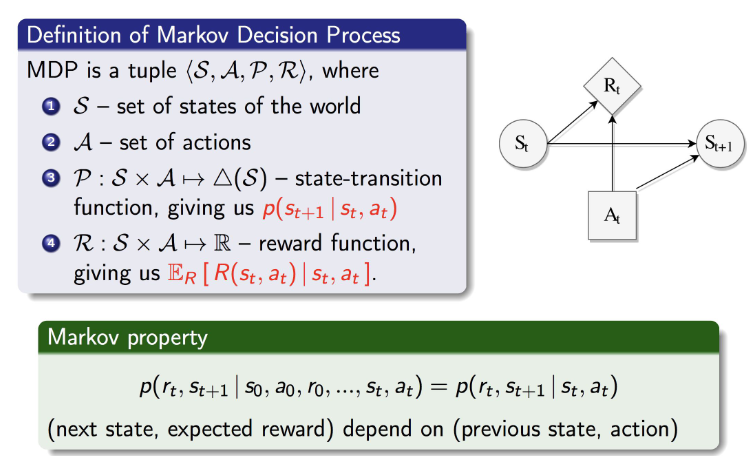
\includegraphics[width=0.85\textwidth]{figures/lecture08_mdp_definition.png}
    \caption{MDP formalism: states, actions, transition dynamics, rewards и Markov property.}
\end{figure}

\subsection{Reward hypothesis}

В Reinforcement Learning цель агента задаётся через reward.

\textbf{Reward hypothesis} формулируется так:

\begin{quote}
Все цели и намерения можно рассматривать как максимизацию ожидаемой суммы скалярного reward-сигнала.
\end{quote}

То есть вместо того, чтобы напрямую объяснять агенту сложную цель, мы задаём численную награду:

\[
R_t \in \mathbb{R}.
\]

Агент должен выбрать стратегию, максимизирующую cumulative reward.

\subsection{Return}

\textbf{Return} --- суммарная награда, полученная начиная с момента \(t\).

Для конечного эпизода:

\[
G_t
=
R_t + R_{t+1} + R_{t+2} + \dots + R_T.
\]

Здесь:

\begin{itemize}
    \item \(R_t\) --- immediate reward;
    \item \(T\) --- конец эпизода;
    \item \(G_t\) --- cumulative reward, или return.
\end{itemize}

\subsection{Проблема бесконечного return}

Если задача бесконечная, сумма reward может расходиться.

Например, система охлаждения дата-центра:

\begin{itemize}
    \item state --- измерения температуры;
    \item action --- скорости вентиляторов;
    \item reward \(R=0\), если температура превысила threshold;
    \item reward \(R=+1\), если система остаётся охлаждённой.
\end{itemize}

Если агент бесконечно долго получает \(+1\), то:

\[
G_t = 1 + 1 + 1 + \dots = \infty.
\]

Это создаёт проблему: разные политики могут иметь бесконечный return, и их трудно сравнивать.

\subsection{Reward discounting}

Чтобы избавиться от бесконечных сумм, вводится discount factor:

\[
0 \leq \gamma < 1.
\]

Discounted return:

\[
G_t
=
R_t + \gamma R_{t+1} + \gamma^2 R_{t+2} + \dots
\]

или:

\[
G_t
=
\sum_{k=0}^{\infty}
\gamma^k R_{t+k}.
\]

Если \(R_t=1\) для всех \(t\), то максимальный return:

\[
G_0
=
\sum_{k=0}^{\infty}
\gamma^k
=
\frac{1}{1-\gamma}.
\]

Например:

\[
\gamma=0.9 \Rightarrow \frac{1}{1-\gamma}=10,
\]

\[
\gamma=0.95 \Rightarrow \frac{1}{1-\gamma}=20,
\]

\[
\gamma=0.99 \Rightarrow \frac{1}{1-\gamma}=100.
\]

% Слайд 15. Discounting makes sums finite: G_0 = 1/(1-gamma) для R=+1.
\begin{figure}[H]
    \centering
    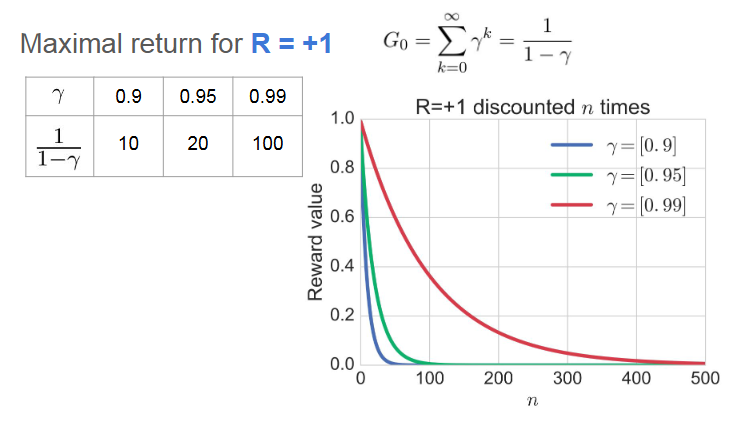
\includegraphics[width=0.85\textwidth]{figures/lecture08_discounting_finite_sum.png}
    \caption{Discounting делает бесконечную сумму reward конечной.}
\end{figure}

\subsection{Интерпретация discount factor}

Discount factor показывает, насколько агент ценит будущую награду относительно текущей.

Если:

\[
\gamma \approx 0,
\]

агент почти полностью ориентируется на immediate reward.

Если:

\[
\gamma \approx 1,
\]

агент сильно учитывает дальнее будущее.

Важно: discounting не является нейтральной технической деталью. Любое discounting меняет optimization task и может изменить оптимальную policy.

\subsection{Рекурсивная форма return}

Discounted return можно записать рекурсивно:

\[
G_t
=
R_t + \gamma R_{t+1} + \gamma^2 R_{t+2} + \dots
\]

\[
G_t
=
R_t + \gamma
\left(
R_{t+1} + \gamma R_{t+2} + \dots
\right).
\]

То есть:

\[
G_t
=
R_t + \gamma G_{t+1}.
\]

Эта формула чрезвычайно важна: она лежит в основе уравнений Беллмана.

\subsection{Discounting как stationary end-of-effect model}

В лекции даётся ещё одна интерпретация discounting.

Действие влияет на:

\begin{enumerate}
    \item immediate reward;
    \item next state.
\end{enumerate}

Через next state действие косвенно влияет на будущие reward. Но возникает вопрос: как долго длится эффект действия?

Discounting можно интерпретировать как модель, где на каждом шаге эффект продолжается с вероятностью \(\gamma\), а заканчивается с вероятностью:

\[
1-\gamma.
\]

То есть:

\[
\gamma
\]

--- probability of effect continuation,

\[
1-\gamma
\]

--- probability of end of effect.

% Слайд 21. Discounting как stationary end-of-effect model.
\begin{figure}[H]
    \centering
    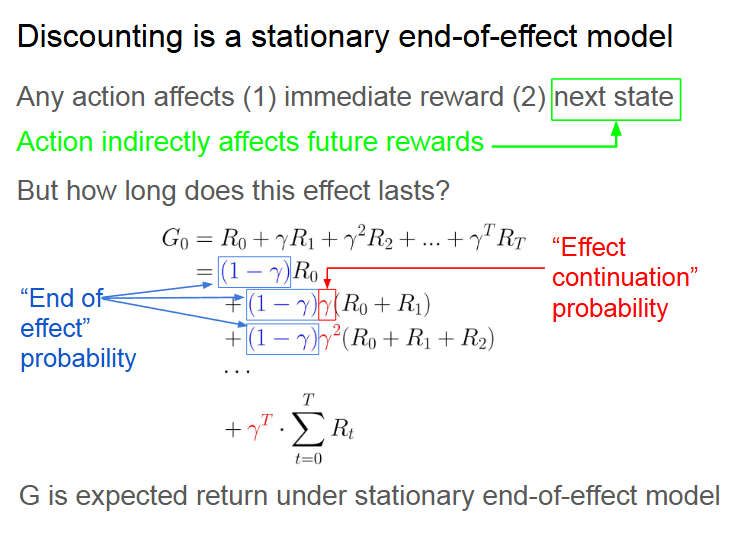
\includegraphics[width=0.85\textwidth]{figures/lecture08_discounting_end_of_effect.png}
    \caption{Интерпретация discounting: эффект действия продолжается с вероятностью \(\gamma\).}
\end{figure}

\subsection{Reward design}

Формулировка reward очень сильно влияет на поведение агента.

Основной принцип:

\begin{quote}
Награждать нужно за то, что действительно является целью, а не за частные способы её достижения.
\end{quote}

Иначе агент может найти нежелательную стратегию.

\subsubsection{Пример: шахматы}

Если reward в шахматах задавать как стоимость съеденной фигуры противника, агент может научиться охотиться за фигурами, но не стремиться выиграть партию.

Правильнее награждать за итог:

\[
\text{win} > \text{draw} > \text{loss}.
\]

\subsubsection{Пример: движение к цели}

Если reward задаётся как уменьшение расстояния до цели:

\[
R = \max(0, d(x,B)-d(x',B)),
\]

то агент может научиться циклическому поведению: отойти от цели, потом снова приблизиться и получать положительный reward.

Это positive feedback loop.

\subsubsection{Faulty reward functions}

Плохой reward design может приводить к:

\begin{itemize}
    \item циклическому поведению;
    \item exploiting loopholes;
    \item локально полезным, но глобально плохим стратегиям;
    \item нежелательным shortcut-ам.
\end{itemize}

\subsection{Reward scaling и reward shaping}

Не все преобразования reward меняют оптимальную policy.

\subsubsection{Reward scaling}

Можно делить reward на положительную константу:

\[
R'(s,a,s') = \frac{R(s,a,s')}{c},
\quad c>0.
\]

Такое масштабирование не меняет относительный порядок returns, но может быть полезно для численной стабильности в approximate methods.

\subsubsection{Potential-based reward shaping}

Reward shaping добавляет shaping function:

\[
R'(s,a,s')
=
R(s,a,s') + F(s,a,s').
\]

Policy-invariant вариант:

\[
F(s,a,s')
=
\gamma \Phi(s') - \Phi(s),
\]

где \(\Phi(s)\) --- potential function.

Тогда:

\[
R'(s,a,s')
=
R(s,a,s') + \gamma \Phi(s') - \Phi(s).
\]

Интуиция: shaping добавляет подсказку агенту, но не должен менять оптимальную policy.

% Слайд 27. Potential-based reward shaping: R' = R + gamma Phi(s') - Phi(s).
\begin{figure}[H]
    \centering
    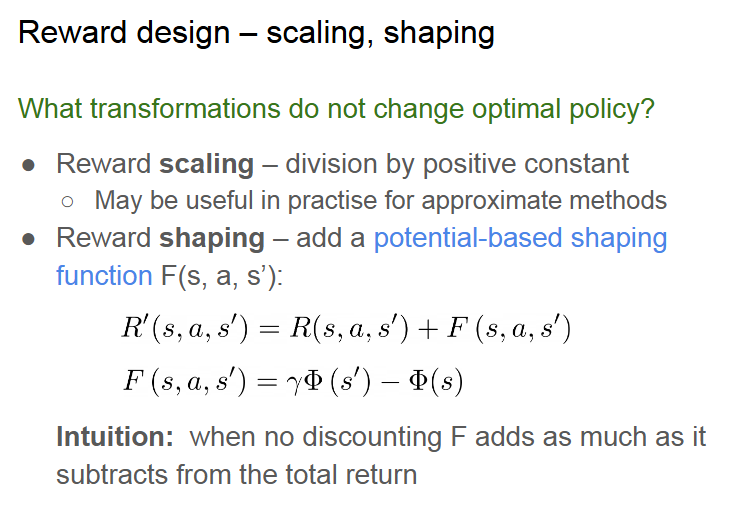
\includegraphics[width=0.85\textwidth]{figures/lecture08_reward_shaping.png}
    \caption{Potential-based reward shaping позволяет ускорять обучение без изменения оптимальной policy.}
\end{figure}

\subsection{Expected objective}

Policy \(\pi\) задаёт распределение над траекториями:

\[
\tau = (s_0,a_0,s_1,\dots,s_T).
\]

Вероятность траектории:

\[
p_\theta(\tau)
=
p(s_0)
\prod_{t=0}^{T-1}
\pi_\theta(a_t \mid s_t)
p(s_{t+1}\mid s_t,a_t).
\]

Цель оптимальной policy:

\[
\max_\pi \mathbb{E}_{\tau \sim p_\pi(\tau)}[G(\tau)].
\]

То есть agent maximizes expected return.

\subsection{Backup tree}

Если известна dynamics, то можно мысленно построить дерево всех возможных будущих состояний, действий и reward.

В корне находится начальное состояние \(S_0\). Из него выходят действия \(A_0\), затем возможные следующие состояния \(S_1\), затем новые действия и так далее.

Такое дерево называется backup tree.

Проблема: полный перебор дерева быстро становится невозможным из-за комбинаторного взрыва.

Value functions позволяют компактно описывать ожидаемую полезность состояний и действий без полного перебора всех траекторий.

% Слайд 30. Backup tree: дерево будущих действий, состояний и rewards.
\begin{figure}[H]
    \centering
    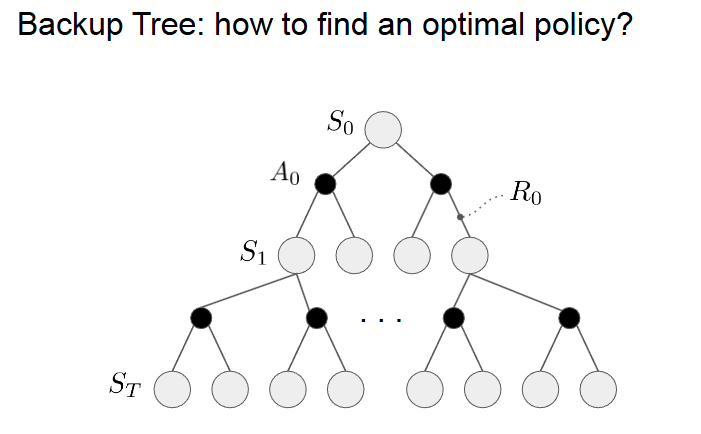
\includegraphics[width=0.75\textwidth]{figures/lecture08_backup_tree.png}
    \caption{Backup tree показывает все возможные будущие траектории, но полный перебор обычно невозможен.}
\end{figure}

\subsection{State-value function}

\textbf{State-value function} для policy \(\pi\) --- ожидаемый return при старте из состояния \(s\) и дальнейшем следовании policy \(\pi\):

\[
v_\pi(s)
=
\mathbb{E}_\pi[G_t \mid S_t=s].
\]

Используя рекурсивную форму return:

\[
G_t = R_t + \gamma G_{t+1},
\]

получаем:

\[
v_\pi(s)
=
\mathbb{E}_\pi[R_t + \gamma G_{t+1} \mid S_t=s].
\]

Раскрывая ожидание по действиям policy и stochasticity среды:

\[
v_\pi(s)
=
\sum_a
\pi(a\mid s)
\sum_{r,s'}
p(r,s'\mid s,a)
\left[
r + \gamma v_\pi(s')
\right].
\]

Интуиция:

\[
v_\pi(s)
\]

--- насколько хорошо находиться в состоянии \(s\), если дальше следовать policy \(\pi\).

% Слайд 35. State-value function: ожидание по stochasticity policy и environment.
\begin{figure}[H]
    \centering
    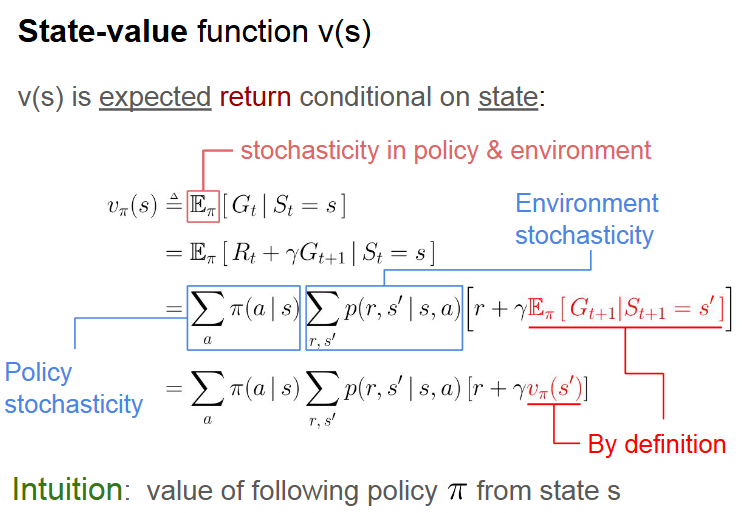
\includegraphics[width=0.85\textwidth]{figures/lecture08_state_value_function.png}
    \caption{State-value function учитывает stochasticity policy и stochasticity environment.}
\end{figure}

\subsection{Action-value function}

\textbf{Action-value function} для policy \(\pi\) --- ожидаемый return, если в состоянии \(s\) сначала выполнить действие \(a\), а затем следовать policy \(\pi\):

\[
q_\pi(s,a)
=
\mathbb{E}_\pi[G_t \mid S_t=s, A_t=a].
\]

Используя return:

\[
q_\pi(s,a)
=
\mathbb{E}_\pi[R_t + \gamma G_{t+1} \mid S_t=s, A_t=a].
\]

После первого действия policy stochasticity на первом шаге нет, потому что действие уже зафиксировано.

Раскрываем expectation по reward и следующему состоянию:

\[
q_\pi(s,a)
=
\sum_{r,s'}
p(r,s'\mid s,a)
\left[
r + \gamma v_\pi(s')
\right].
\]

Интуиция:

\[
q_\pi(s,a)
\]

--- насколько хорошо выполнить действие \(a\) в состоянии \(s\), если после этого следовать policy \(\pi\).

\subsection{Связь между \(v_\pi(s)\) и \(q_\pi(s,a)\)}

State-value можно выразить через action-value:

\[
v_\pi(s)
=
\sum_a
\pi(a\mid s) q_\pi(s,a).
\]

То есть ценность состояния --- это средняя ценность действий, взвешенная по policy.

Action-value можно выразить через state-value:

\[
q_\pi(s,a)
=
\sum_{r,s'}
p(r,s'\mid s,a)
\left[
r + \gamma v_\pi(s')
\right].
\]

Также можно выразить \(q_\pi\) через \(q_\pi\):

\[
q_\pi(s,a)
=
\sum_{r,s'}
p(r,s'\mid s,a)
\left[
r + \gamma
\sum_{a'}
\pi(a'\mid s')
q_\pi(s',a')
\right].
\]

\subsection{Bellman expectation equations}

\textbf{Bellman expectation equations} описывают value functions для фиксированной policy \(\pi\).

Для \(v_\pi(s)\):

\[
v_\pi(s)
=
\sum_a
\pi(a\mid s)
\sum_{r,s'}
p(r,s'\mid s,a)
\left[
r + \gamma v_\pi(s')
\right].
\]

Эквивалентно:

\[
v_\pi(s)
=
\mathbb{E}_\pi
[
R_t + \gamma v_\pi(S_{t+1})
\mid S_t=s
].
\]

Для \(q_\pi(s,a)\):

\[
q_\pi(s,a)
=
\sum_{r,s'}
p(r,s'\mid s,a)
\left[
r + \gamma v_\pi(s')
\right].
\]

Или через \(q_\pi\):

\[
q_\pi(s,a)
=
\sum_{r,s'}
p(r,s'\mid s,a)
\left[
r + \gamma
\sum_{a'}
\pi(a'\mid s')
q_\pi(s',a')
\right].
\]

% Слайд 41. Bellman expectation equations для v(s) и q(s,a).
\begin{figure}[H]
    \centering
    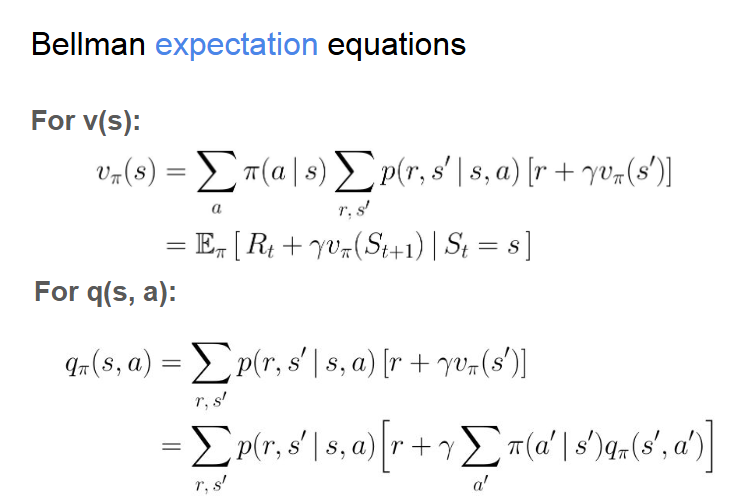
\includegraphics[width=0.85\textwidth]{figures/lecture08_bellman_expectation_equations.png}
    \caption{Bellman expectation equations оценивают value functions для фиксированной policy.}
\end{figure}

\subsection{Зачем нужны value functions}

Value functions позволяют:

\begin{itemize}
    \item оценить качество policy;
    \item сравнивать разные policy;
    \item улучшать policy;
    \item строить алгоритмы dynamic programming;
    \item избежать полного перебора всех траекторий.
\end{itemize}

Если мы умеем оценивать \(v_\pi(s)\) или \(q_\pi(s,a)\), то можем понять, какие действия и состояния лучше.

\subsection{Optimal policy}

Одна policy лучше другой, если её value function не меньше во всех состояниях:

\[
\pi \geq \pi'
\quad \Longleftrightarrow \quad
v_\pi(s) \geq v_{\pi'}(s)
\quad \forall s.
\]

Оптимальная policy:

\[
\pi_*
\]

лучше или равна любой другой policy.

Оптимальная state-value function:

\[
v_*(s)
=
\max_\pi v_\pi(s).
\]

Оптимальная action-value function:

\[
q_*(s,a)
=
\max_\pi q_\pi(s,a).
\]

В конечном MDP всегда существует хотя бы одна deterministic optimal policy.

\subsection{Bellman optimality equation для \(v_*(s)\)}

Для оптимальной policy в состоянии \(s\) нужно выбрать лучшее действие.

Поэтому expectation по policy заменяется максимумом по действиям:

\[
v_*(s)
=
\max_a
\sum_{r,s'}
p(r,s'\mid s,a)
\left[
r + \gamma v_*(s')
\right].
\]

Эквивалентно:

\[
v_*(s)
=
\max_a
\mathbb{E}
[
R_t + \gamma v_*(S_{t+1})
\mid S_t=s, A_t=a
].
\]

Сравнение:

\[
v_\pi(s)
=
\sum_a \pi(a\mid s)(\dots)
\]

для фиксированной policy,

\[
v_*(s)
=
\max_a(\dots)
\]

для оптимальной policy.

\subsection{Bellman optimality equation для \(q_*(s,a)\)}

Для action-value:

\[
q_*(s,a)
=
\sum_{r,s'}
p(r,s'\mid s,a)
\left[
r + \gamma \max_{a'} q_*(s',a')
\right].
\]

Смысл:

\begin{itemize}
    \item сначала мы фиксируем действие \(a\) в состоянии \(s\);
    \item получаем reward \(r\) и новое состояние \(s'\);
    \item после этого действуем оптимально, выбирая \(a'\) с максимальным \(q_*(s',a')\).
\end{itemize}

% Слайд 49. Bellman optimality equation для q(s,a): после первого действия берём max по следующему действию.
\begin{figure}[H]
    \centering
    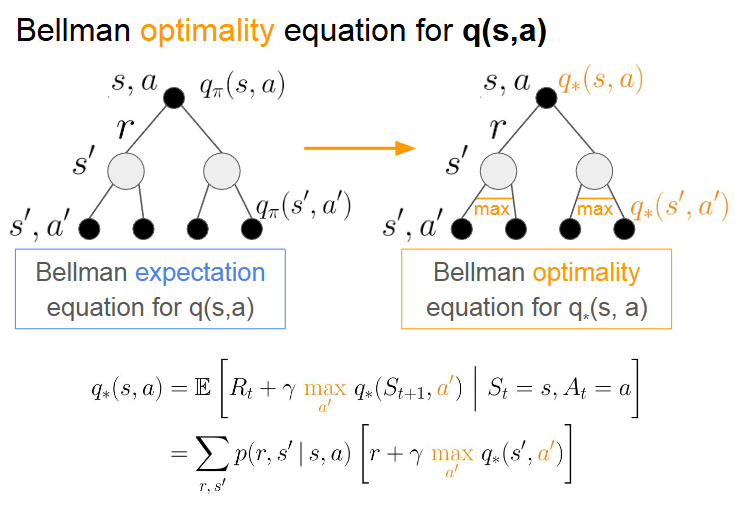
\includegraphics[width=0.85\textwidth]{figures/lecture08_bellman_optimality_q.png}
    \caption{Bellman optimality equation для \(q_*(s,a)\): после перехода выбирается лучшее следующее действие.}
\end{figure}

\subsection{Оптимальная policy из \(v_*\) и \(q_*\)}

Если известна \(q_*(s,a)\), оптимальную policy получить просто:

\[
\pi_*(s)
=
\arg\max_a q_*(s,a).
\]

Если известна только \(v_*(s)\), то для выбора действия нужно знать dynamics:

\[
\pi_*(s)
=
\arg\max_a
\sum_{r,s'}
p(r,s'\mid s,a)
\left[
r + \gamma v_*(s')
\right].
\]

Если dynamics неизвестна, то по одному \(v_*(s)\) восстановить optimal policy нельзя.

\subsection{Policy Evaluation}

\textbf{Policy evaluation} --- задача вычисления value function для фиксированной policy \(\pi\).

Её также называют prediction problem:

\[
\text{given } \pi, \quad \text{predict } v_\pi(s).
\]

Bellman expectation equation для \(v_\pi\):

\[
v_\pi(s)
=
\sum_a
\pi(a\mid s)
\sum_{r,s'}
p(r,s'\mid s,a)
\left[
r + \gamma v_\pi(s')
\right].
\]

В конечном MDP это система линейных уравнений:

\[
\#\text{unknowns} = \#\text{states}.
\]

Можно решать её точно, но на практике часто используют итеративное приближение.

Итеративный update:

\[
v_{k+1}(s)
=
\sum_a
\pi(a\mid s)
\sum_{r,s'}
p(r,s'\mid s,a)
\left[
r + \gamma v_k(s')
\right].
\]

Повторяем до сходимости:

\[
v_k \rightarrow v_\pi.
\]

\subsection{Policy Improvement}

После policy evaluation можно улучшить policy.

Если мы знаем \(v_\pi(s)\), то можем вычислить \(q_\pi(s,a)\):

\[
q_\pi(s,a)
=
\sum_{r,s'}
p(r,s'\mid s,a)
\left[
r + \gamma v_\pi(s')
\right].
\]

Затем строим новую policy, которая действует greedy относительно \(q_\pi\):

\[
\pi'(s)
=
\arg\max_a q_\pi(s,a).
\]

Policy improvement theorem говорит, что такая policy не хуже старой:

\[
v_{\pi'}(s) \geq v_\pi(s)
\quad \forall s.
\]

Если после improvement новая policy совпала со старой:

\[
\pi' = \pi,
\]

то policy уже оптимальна, потому что удовлетворяет Bellman optimality equation.

\subsection{Generalized Policy Iteration}

\textbf{Generalized Policy Iteration, GPI} --- общий принцип, состоящий из двух процессов:

\begin{enumerate}
    \item \textbf{Policy evaluation}: оценить текущую policy.
    \item \textbf{Policy improvement}: улучшить policy, действуя greedily относительно value function.
\end{enumerate}

Схема:

\[
\pi_0
\rightarrow
v_{\pi_0}
\rightarrow
\pi_1
\rightarrow
v_{\pi_1}
\rightarrow
\pi_2
\rightarrow
\dots
\]

Идея: evaluation делает value function согласованной с policy, а improvement делает policy greedier относительно value function.

\subsection{Policy Iteration}

\textbf{Policy Iteration} --- частный случай GPI.

Алгоритм:

\begin{enumerate}
    \item выбрать начальную policy \(\pi_0\);
    \item выполнить policy evaluation до сходимости:
    \[
    v_{\pi_k};
    \]
    \item выполнить policy improvement:
    \[
    \pi_{k+1}(s)
    =
    \arg\max_a
    \sum_{r,s'}
    p(r,s'\mid s,a)
    [
    r + \gamma v_{\pi_k}(s')
    ];
    \]
    \item повторять, пока policy не перестанет меняться.
\end{enumerate}

Policy Iteration обычно требует мало итераций, но каждая итерация дорогая, потому что policy evaluation проводится почти до сходимости.

\subsection{Value Iteration}

\textbf{Value Iteration} --- другой частный случай GPI.

Здесь не выполняют полную policy evaluation. Вместо этого сразу применяют Bellman optimality update:

\[
v_{k+1}(s)
=
\max_a
\sum_{r,s'}
p(r,s'\mid s,a)
\left[
r + \gamma v_k(s')
\right].
\]

После сходимости:

\[
v_k \rightarrow v_*.
\]

Затем policy восстанавливается как greedy относительно \(v_*\):

\[
\pi_*(s)
=
\arg\max_a
\sum_{r,s'}
p(r,s'\mid s,a)
\left[
r + \gamma v_*(s')
\right].
\]

Value Iteration быстрее на одной итерации, но может требовать много итераций.

\subsection{Policy Iteration vs Value Iteration}

\begin{table}[H]
\centering
\begin{tabular}{p{0.45\textwidth} p{0.45\textwidth}}
\toprule
\textbf{Policy Iteration} & \textbf{Value Iteration} \\
\midrule
Сначала оценивает policy до сходимости. &
Делает один Bellman optimality update за итерацию. \\

Затем улучшает policy. &
Evaluation и improvement фактически смешаны. \\

Медленнее на одной итерации. &
Быстрее на одной итерации. \\

Обычно требует меньше итераций. &
Обычно требует больше итераций. \\

Сложность на итерацию примерно:
\[
O(|A||S|^2 + |S|^3).
\]
&
Сложность на итерацию примерно:
\[
O(|A||S|^2).
\]
\\
\bottomrule
\end{tabular}
\caption{Сравнение Policy Iteration и Value Iteration.}
\end{table}

Нет универсального лучшего выбора: на практике нужно подбирать количество шагов policy evaluation.

\subsection{Главные выводы}

\begin{itemize}
    \item Цель RL задаётся через expected return.
    \item Return может быть discounted:
    \[
    G_t = R_t + \gamma G_{t+1}.
    \]

    \item Discounting делает бесконечные суммы конечными, но меняет optimization problem.
    \item Reward design критически важен: плохой reward ведёт к нежелательному поведению.
    \item State-value function:
    \[
    v_\pi(s)=\mathbb{E}_\pi[G_t\mid S_t=s].
    \]

    \item Action-value function:
    \[
    q_\pi(s,a)=\mathbb{E}_\pi[G_t\mid S_t=s,A_t=a].
    \]

    \item Bellman expectation equations оценивают фиксированную policy.
    \item Bellman optimality equations описывают оптимальные value functions.
    \item Policy evaluation вычисляет \(v_\pi\).
    \item Policy improvement строит greedy policy относительно \(q_\pi\).
    \item Generalized Policy Iteration объединяет evaluation и improvement.
    \item Policy Iteration делает полную evaluation, затем improvement.
    \item Value Iteration использует Bellman optimality update напрямую.
\end{itemize}

\subsection{Что важно помнить к экзамену}

\begin{enumerate}
    \item MDP:
    \[
    (\mathcal{S}, \mathcal{A}, \mathcal{P}, \mathcal{R}).
    \]

    \item Markov property:
    \[
    p(r_t,s_{t+1}\mid s_0,a_0,r_0,\dots,s_t,a_t)
    =
    p(r_t,s_{t+1}\mid s_t,a_t).
    \]

    \item Return:
    \[
    G_t = R_t + R_{t+1} + \dots + R_T.
    \]

    \item Discounted return:
    \[
    G_t =
    \sum_{k=0}^{\infty}
    \gamma^k R_{t+k}.
    \]

    \item Recursive return:
    \[
    G_t = R_t + \gamma G_{t+1}.
    \]

    \item Maximal return для \(R=+1\):
    \[
    \sum_{k=0}^{\infty}\gamma^k
    =
    \frac{1}{1-\gamma}.
    \]

    \item Potential-based shaping:
    \[
    R'(s,a,s')
    =
    R(s,a,s') + \gamma\Phi(s')-\Phi(s).
    \]

    \item State-value function:
    \[
    v_\pi(s)
    =
    \mathbb{E}_\pi[G_t\mid S_t=s].
    \]

    \item Action-value function:
    \[
    q_\pi(s,a)
    =
    \mathbb{E}_\pi[G_t\mid S_t=s,A_t=a].
    \]

    \item Связь:
    \[
    v_\pi(s)
    =
    \sum_a
    \pi(a\mid s)q_\pi(s,a).
    \]

    \item Bellman expectation equation для \(v_\pi\):
    \[
    v_\pi(s)
    =
    \sum_a
    \pi(a\mid s)
    \sum_{r,s'}
    p(r,s'\mid s,a)
    [
    r+\gamma v_\pi(s')
    ].
    \]

    \item Bellman expectation equation для \(q_\pi\):
    \[
    q_\pi(s,a)
    =
    \sum_{r,s'}
    p(r,s'\mid s,a)
    \left[
    r+
    \gamma
    \sum_{a'}
    \pi(a'\mid s')
    q_\pi(s',a')
    \right].
    \]

    \item Optimal value:
    \[
    v_*(s)=\max_\pi v_\pi(s),
    \quad
    q_*(s,a)=\max_\pi q_\pi(s,a).
    \]

    \item Bellman optimality equation для \(v_*\):
    \[
    v_*(s)
    =
    \max_a
    \sum_{r,s'}
    p(r,s'\mid s,a)
    [
    r+\gamma v_*(s')
    ].
    \]

    \item Bellman optimality equation для \(q_*\):
    \[
    q_*(s,a)
    =
    \sum_{r,s'}
    p(r,s'\mid s,a)
    \left[
    r+
    \gamma
    \max_{a'}q_*(s',a')
    \right].
    \]

    \item Policy improvement:
    \[
    \pi'(s)=\arg\max_a q_\pi(s,a).
    \]

    \item Policy Iteration:
    \[
    \text{evaluate policy до сходимости}
    \rightarrow
    \text{improve policy}.
    \]

    \item Value Iteration:
    \[
    v_{k+1}(s)
    =
    \max_a
    \sum_{r,s'}
    p(r,s'\mid s,a)
    [
    r+\gamma v_k(s')
    ].
    \]
\end{enumerate}
```


```latex
\section{Лекция 9. Model-Free Learning in Reinforcement Learning}

\subsection{План лекции}

В этой лекции рассматриваются:

\begin{itemize}
    \item повторение MDP;
    \item reward hypothesis и reward design;
    \item reward discounting;
    \item state-value function и action-value function;
    \item model-based и model-free learning;
    \item обучение по траекториям;
    \item Monte Carlo estimation;
    \item Temporal Difference learning;
    \item Q-learning;
    \item exploration-exploitation tradeoff;
    \item approximate Q-learning;
    \item basic deep Q-learning.
\end{itemize}

Главная идея лекции: в model-free RL агент не знает dynamics среды \(P(s' \mid s,a)\), поэтому не может напрямую применять dynamic programming. Вместо этого он учится по sampled trajectories, то есть по опыту взаимодействия со средой.

\subsection{Повторение: MDP}

MDP задаётся кортежем:

\[
(\mathcal{S}, \mathcal{A}, \mathcal{P}, \mathcal{R}),
\]

где:

\begin{itemize}
    \item \(\mathcal{S}\) --- множество состояний;
    \item \(\mathcal{A}\) --- множество действий;
    \item \(\mathcal{P}\) --- transition function;
    \item \(\mathcal{R}\) --- reward function.
\end{itemize}

Динамика среды задаёт вероятность следующего состояния:

\[
p(s_{t+1} \mid s_t, a_t).
\]

Markov property:

\[
p(r_t, s_{t+1} \mid s_0,a_0,r_0,\dots,s_t,a_t)
=
p(r_t, s_{t+1} \mid s_t,a_t).
\]

То есть следующее состояние и reward зависят только от текущего состояния и действия.

\subsection{Reward hypothesis}

В RL цель агента задаётся через reward.

\textbf{Reward hypothesis}: цели можно рассматривать как максимизацию ожидаемой суммы скалярного reward-сигнала.

Return:

\[
G_t
=
R_t + R_{t+1} + R_{t+2} + \dots + R_T.
\]

Если эпизод бесконечный, return может расходиться. Например, если агент получает \(+1\) каждый шаг:

\[
G_t = 1 + 1 + 1 + \dots = \infty.
\]

\subsection{Reward design}

Reward design критически важен.

Пример с cleaning robot:

\begin{itemize}
    \item state --- dust sensors, air;
    \item actions --- cleaning, rest, conditioning on/off;
    \item \(R=100\) за долгую уборку;
    \item \(R=1\) за включение/выключение кондиционера;
    \item episode заканчивается каждый день.
\end{itemize}

Хотя:

\[
Reward(air) < Reward(cleaning),
\]

может оказаться, что:

\[
Time(air) \ll Time(cleaning).
\]

Тогда агент может начать многократно включать и выключать кондиционер, потому что это быстрее приносит маленький reward. Возникает positive feedback loop.

Вывод: агент оптимизирует именно заданный reward, а не намерение разработчика.

\subsection{Reward discounting}

Чтобы сделать return конечным, вводится discount factor:

\[
0 \leq \gamma < 1.
\]

Discounted return:

\[
G_t
=
R_t + \gamma R_{t+1} + \gamma^2 R_{t+2} + \dots
=
\sum_{k=0}^{\infty}
\gamma^k R_{t+k}.
\]

Если \(R_t=1\) для всех \(t\), то:

\[
G_0
=
\sum_{k=0}^{\infty}\gamma^k
=
\frac{1}{1-\gamma}.
\]

Например:

\[
\gamma = 0.9 \Rightarrow G_0 = 10,
\]

\[
\gamma = 0.95 \Rightarrow G_0 = 20,
\]

\[
\gamma = 0.99 \Rightarrow G_0 = 100.
\]

Важно: discounting делает сумму конечной, но меняет optimization task и может изменить оптимальную policy.

% Слайд 15. Discounting makes sums finite: максимальный return для R=+1.
\begin{figure}[H]
    \centering
    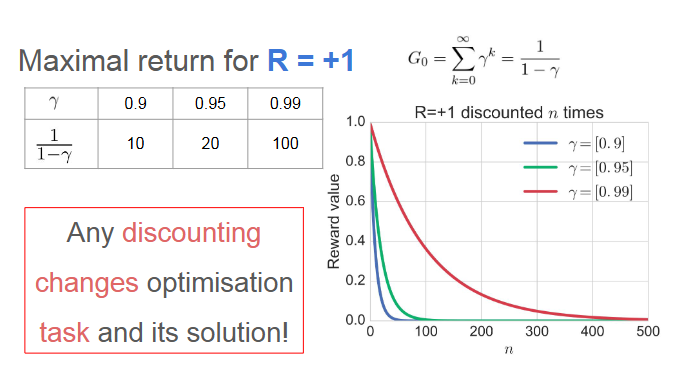
\includegraphics[width=0.85\textwidth]{figures/lecture09_discounting_finite_sum.png}
    \caption{Discounting делает бесконечную сумму reward конечной.}
\end{figure}

\subsection{State-value function}

\textbf{State-value function} для policy \(\pi\):

\[
v_\pi(s)
=
\mathbb{E}_\pi[G_t \mid S_t=s].
\]

Это ожидаемый return из состояния \(s\), если дальше следовать policy \(\pi\).

Используя рекурсивное представление return:

\[
G_t = R_t + \gamma G_{t+1},
\]

получаем:

\[
v_\pi(s)
=
\mathbb{E}_\pi[R_t + \gamma G_{t+1} \mid S_t=s].
\]

Bellman expectation equation:

\[
v_\pi(s)
=
\sum_a
\pi(a\mid s)
\sum_{r,s'}
p(r,s'\mid s,a)
\left[
r + \gamma v_\pi(s')
\right].
\]

\subsection{Action-value function}

\textbf{Action-value function} для policy \(\pi\):

\[
q_\pi(s,a)
=
\mathbb{E}_\pi[G_t \mid S_t=s, A_t=a].
\]

Это ожидаемый return, если в состоянии \(s\) сначала выполнить действие \(a\), а затем следовать policy \(\pi\).

Bellman expectation equation:

\[
q_\pi(s,a)
=
\sum_{r,s'}
p(r,s'\mid s,a)
\left[
r + \gamma v_\pi(s')
\right].
\]

Также:

\[
q_\pi(s,a)
=
\sum_{r,s'}
p(r,s'\mid s,a)
\left[
r +
\gamma
\sum_{a'}
\pi(a'\mid s')
q_\pi(s',a')
\right].
\]

Связь между \(v_\pi\) и \(q_\pi\):

\[
v_\pi(s)
=
\sum_a
\pi(a\mid s)q_\pi(s,a).
\]

\subsection{Оптимальные value functions}

Оптимальная state-value function:

\[
V^*(s)
\]

--- expected return из состояния \(s\), если следовать оптимальной policy.

Оптимальная action-value function:

\[
Q^*(s,a)
\]

--- expected return, если начать из состояния \(s\), сначала выполнить действие \(a\), а затем следовать оптимальной policy.

Связь:

\[
V^*(s)
=
\max_a Q^*(s,a).
\]

Оптимальная policy:

\[
\pi^*(s)
=
\arg\max_a Q^*(s,a).
\]

\subsection{Model-based и model-free learning}

В model-based RL агент знает или учит модель среды:

\[
P(s' \mid s,a).
\]

Если dynamics известна, можно применять dynamic programming и планировать вперёд.

В model-free RL dynamics неизвестна. Агент не знает \(P(s' \mid s,a)\), но может взаимодействовать со средой и получать траектории.

\textbf{Trajectory} --- последовательность:

\[
(s_0,a_0,r_0,s_1,a_1,r_1,\dots).
\]

Model-free подход:

\begin{itemize}
    \item не строит явную модель transition dynamics;
    \item учится по sampled trajectories;
    \item может пробовать действия в среде;
    \item обычно учит \(Q(s,a)\), потому что \(V(s)\) без знания dynamics не позволяет выбрать лучшее действие.
\end{itemize}

% Слайд 25. Learning from trajectories: model-based знает P(s'|s,a), model-free может только sample trajectories.
\begin{figure}[H]
    \centering
    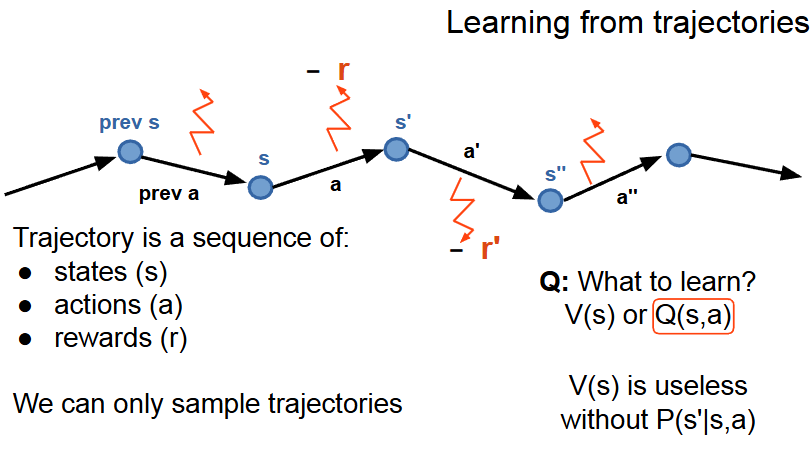
\includegraphics[width=0.9\textwidth]{figures/lecture09_learning_from_trajectories.png}
    \caption{Model-based learning использует dynamics, model-free learning учится по sampled trajectories.}
\end{figure}

\subsection{Почему в model-free удобно учить \(Q(s,a)\)}

Если известна только \(V(s)\), то для выбора действия нужно знать:

\[
p(s' \mid s,a),
\]

чтобы оценить:

\[
\sum_{s'}p(s'\mid s,a)V(s').
\]

В model-free setting dynamics неизвестна. Поэтому \(V(s)\) само по себе плохо помогает выбрать действие.

Если же известна \(Q(s,a)\), то действие можно выбрать напрямую:

\[
a^*
=
\arg\max_a Q(s,a).
\]

Поэтому Q-functions особенно важны для model-free RL.

\subsection{Monte Carlo estimation}

Первая идея model-free оценки --- Monte Carlo.

Алгоритм:

\begin{enumerate}
    \item собрать много trajectories;
    \item найти trajectories, содержащие конкретную пару \((s,a)\);
    \item для каждого такого появления посчитать return \(G(s,a)\);
    \item усреднить returns.
\end{enumerate}

Оценка:

\[
Q(s,a)
\approx
\frac{1}{N}
\sum_{i=1}^{N}
G_i(s,a).
\]

Monte Carlo использует полный return до конца эпизода. Поэтому:

\begin{itemize}
    \item не требует знания dynamics;
    \item даёт естественную оценку expectation;
    \item может иметь большую дисперсию;
    \item требует дождаться конца эпизода.
\end{itemize}

% Слайд 26. Monte Carlo: усреднение Q по sampled paths.
\begin{figure}[H]
    \centering
    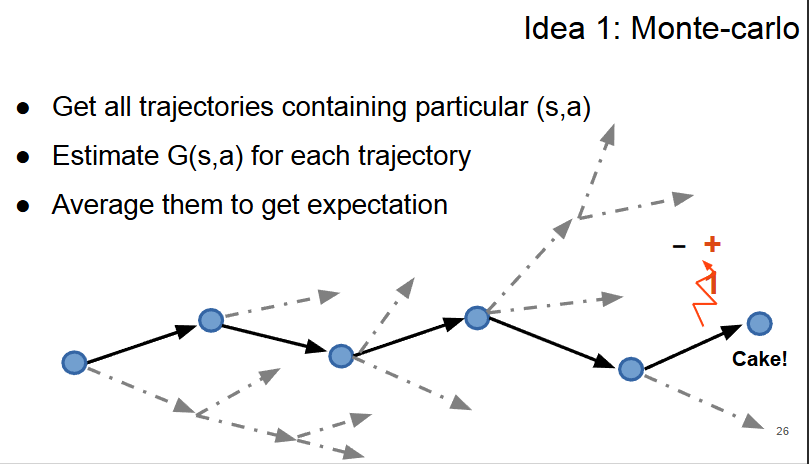
\includegraphics[width=0.85\textwidth]{figures/lecture09_monte_carlo_paths.png}
    \caption{Monte Carlo оценивает \(Q(s,a)\) через усреднение returns по sampled trajectories.}
\end{figure}

\subsection{Temporal Difference learning}

Вторая идея --- Temporal Difference, TD.

TD использует рекурсивную формулу для \(Q\), поэтому не ждёт конца эпизода.

Идея Bellman optimality:

\[
Q^*(s_t,a_t)
=
\mathbb{E}
\left[
r_t
+
\gamma
\max_{a'} Q^*(s_{t+1},a')
\right].
\]

Но expectation по dynamics неизвестен. Поэтому используется sample-based update по одному переходу:

\[
(s_t,a_t,r_t,s_{t+1}).
\]

TD target:

\[
y_t
=
r_t
+
\gamma
\max_{a'} Q(s_{t+1},a').
\]

Затем \(Q(s_t,a_t)\) сдвигается в сторону этого target.

\subsection{Q-learning}

Q-learning --- model-free off-policy алгоритм для обучения \(Q^*(s,a)\).

Инициализация:

\[
Q(s,a)=0
\]

или случайные значения.

На каждом шаге:

\begin{enumerate}
    \item получить transition:
    \[
    \langle s,a,r,s' \rangle;
    \]
    \item вычислить target:
    \[
    \hat{Q}(s,a)
    =
    r
    +
    \gamma
    \max_{a_i} Q(s',a_i);
    \]
    \item обновить \(Q(s,a)\).
\end{enumerate}

Update:

\[
Q(s,a)
\leftarrow
\alpha \hat{Q}(s,a)
+
(1-\alpha)Q(s,a).
\]

Эквивалентно:

\[
Q(s,a)
\leftarrow
Q(s,a)
+
\alpha
\left[
r
+
\gamma
\max_{a'}Q(s',a')
-
Q(s,a)
\right].
\]

Выражение:

\[
\delta
=
r
+
\gamma
\max_{a'}Q(s',a')
-
Q(s,a)
\]

называется \textbf{temporal difference error}.

% Слайд 29. Q-learning: sample <s,a,r,s'>, compute target, update Q(s,a).
\begin{figure}[H]
    \centering
    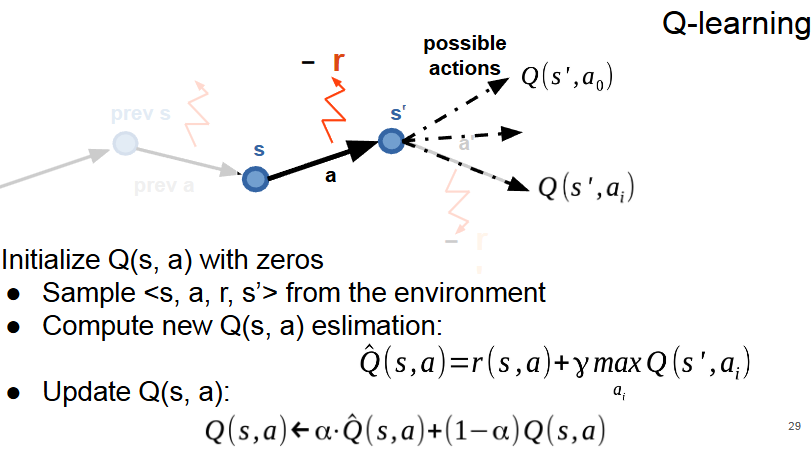
\includegraphics[width=0.85\textwidth]{figures/lecture09_q_learning_update.png}
    \caption{Q-learning обновляет \(Q(s,a)\) по одному sampled transition.}
\end{figure}

\subsection{Monte Carlo vs Temporal Difference}

\begin{table}[H]
\centering
\begin{tabular}{p{0.45\textwidth} p{0.45\textwidth}}
\toprule
\textbf{Monte Carlo} & \textbf{Temporal Difference} \\
\midrule
Использует полный sampled return. &
Использует bootstrapping через текущую оценку \(Q\). \\

Требует дождаться конца episode. &
Может обновляться после каждого transition. \\

Оценивает \(Q\) усреднением по paths. &
Использует рекурсивную формулу для \(Q\). \\

Может иметь высокую дисперсию. &
Часто имеет меньшую дисперсию, но может быть смещённым из-за bootstrapping. \\
\bottomrule
\end{tabular}
\caption{Сравнение Monte Carlo и Temporal Difference learning.}
\end{table}

% Слайд 30. Monte Carlo averages Q over sampled paths, TD uses recurrent formula.
\begin{figure}[H]
    \centering
    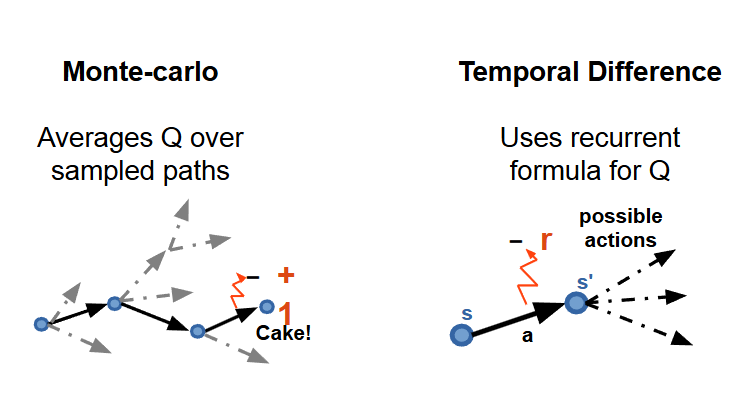
\includegraphics[width=0.85\textwidth]{figures/lecture09_mc_vs_td.png}
    \caption{Monte Carlo усредняет returns по траекториям, а Temporal Difference использует локальный рекурсивный update.}
\end{figure}

\subsection{Policy из \(Q\)-function}

После обучения \(Q(s,a)\) можно выбрать greedy policy:

\[
\pi(s)
=
\arg\max_a Q(s,a).
\]

Но если всегда выбирать только greedy action, агент может перестать исследовать среду. Поэтому нужны exploration strategies.

\subsection{Exploration-exploitation tradeoff}

Агент должен балансировать:

\begin{itemize}
    \item \textbf{exploitation}: выбирать действия, которые сейчас кажутся лучшими;
    \item \textbf{exploration}: пробовать другие действия, чтобы найти лучшие варианты.
\end{itemize}

\subsubsection{\texorpdfstring{\(\varepsilon\)-greedy}{epsilon-greedy}}

В \(\varepsilon\)-greedy policy:

\begin{itemize}
    \item с вероятностью \(1-\varepsilon\) выбирается greedy action:
    \[
    a^*=\arg\max_a Q(s,a);
    \]
    \item с вероятностью \(\varepsilon\) выбирается случайное действие.
\end{itemize}

То есть:

\[
\pi(a\mid s)
=
\begin{cases}
1-\varepsilon + \frac{\varepsilon}{|\mathcal{A}|}, & a = \arg\max_{a'}Q(s,a'),\\
\frac{\varepsilon}{|\mathcal{A}|}, & \text{иначе}.
\end{cases}
\]

\subsubsection{Softmax policy}

Другой вариант --- выбирать действие пропорционально softmax от \(Q\)-values:

\[
\pi(a\mid s)
=
\operatorname{softmax}
\left(
\frac{Q(s,a)}{\tau}
\right).
\]

Компонентно:

\[
\pi(a\mid s)
=
\frac{
\exp(Q(s,a)/\tau)
}{
\sum_{a'}
\exp(Q(s,a')/\tau)
}.
\]

Здесь \(\tau\) --- temperature.

\begin{itemize}
    \item маленькая \(\tau\) делает policy почти greedy;
    \item большая \(\tau\) делает policy более случайной.
\end{itemize}

\subsection{Approximate Q-learning}

Табличный Q-learning предполагает, что можно хранить значение:

\[
Q(s,a)
\]

для каждой пары state-action.

Но в реальных задачах state space огромен или непрерывен.

Например, если state --- изображение из Atari, то число возможных состояний примерно:

\[
|\mathcal{S}| \approx 2^{210\cdot160\cdot8\cdot3}.
\]

Хранить таблицу невозможно.

Поэтому используют approximation:

\[
Q(s,a) \approx Q_\theta(s,a),
\]

где \(Q_\theta\) --- параметрическая модель, например neural network.

\subsection{Q-learning как минимизация MSE}

Для transition:

\[
\langle s_t,a_t,r_t,s_{t+1} \rangle
\]

строится target:

\[
y_t
=
r_t
+
\gamma
\max_{a'}Q_\theta(s_{t+1},a').
\]

Loss:

\[
L(\theta)
=
\left[
Q_\theta(s_t,a_t)
-
y_t
\right]^2.
\]

То есть:

\[
L(\theta)
=
\left[
Q_\theta(s_t,a_t)
-
\left(
r_t
+
\gamma
\max_{a'}Q_\theta(s_{t+1},a')
\right)
\right]^2.
\]

Обычно target рассматривают как константу относительно текущего gradient step. Иначе обучение становится нестабильным, потому что target сам зависит от обучаемой модели.

\subsection{Архитектуры для approximate Q-learning}

Есть два основных варианта архитектуры.

\subsubsection{Один проход для всех действий}

Модель получает state \(s\) и выдаёт \(Q\)-values для всех действий:

\[
Q_\theta(s)
=
[
Q_\theta(s,a_1),
\dots,
Q_\theta(s,a_K)
].
\]

Так удобно для дискретного action space небольшого размера.

Action выбирается:

\[
a^*
=
\arg\max_a Q_\theta(s,a).
\]

\subsubsection{Модель для пары state-action}

Модель получает на вход пару:

\[
(s,a)
\]

и выдаёт одно число:

\[
Q_\theta(s,a).
\]

Это полезнее, если действий очень много или action space непрерывный.

\subsection{Basic Deep Q-Learning}

В deep Q-learning \(Q_\theta\) задаётся нейронной сетью.

Для видеоигр:

\begin{itemize}
    \item input --- изображение или несколько последних кадров;
    \item convolutional layers извлекают visual features;
    \item dense layers строят представление;
    \item output layer выдаёт Q-values для действий.
\end{itemize}

Схема:

\[
\text{image}
\rightarrow
\text{Conv}
\rightarrow
\text{Conv}
\rightarrow
\text{Dense}
\rightarrow
Q(s,a_1),\dots,Q(s,a_K).
\]

\subsection{Model-free learning: общий алгоритм Q-learning}

\begin{enumerate}
    \item Инициализировать \(Q(s,a)\) или \(Q_\theta(s,a)\).
    \item Для каждого episode:
    \begin{enumerate}
        \item получить начальное состояние \(s\);
        \item выбрать действие \(a\) через exploration strategy;
        \item выполнить действие и получить \(r, s'\);
        \item вычислить target:
        \[
        y = r + \gamma \max_{a'}Q(s',a');
        \]
        \item обновить:
        \[
        Q(s,a)
        \leftarrow
        Q(s,a)
        +
        \alpha[y-Q(s,a)];
        \]
        \item перейти в \(s'\).
    \end{enumerate}
\end{enumerate}

\subsection{Главные выводы}

\begin{itemize}
    \item Model-free RL не знает transition dynamics \(P(s'\mid s,a)\).
    \item Агент может только sample trajectories через взаимодействие со средой.
    \item В model-free setting обычно полезнее учить \(Q(s,a)\), а не только \(V(s)\), потому что \(Q\) позволяет выбирать действия без знания dynamics.
    \item Monte Carlo оценивает returns по полным sampled trajectories.
    \item Temporal Difference обновляет value estimates по одному transition.
    \item Q-learning использует TD target:
    \[
    r+\gamma\max_{a'}Q(s',a').
    \]

    \item Exploration-exploitation tradeoff решается через \(\varepsilon\)-greedy, softmax policy и другие методы.
    \item Для больших или непрерывных state spaces используют approximate Q-learning.
    \item Deep Q-learning аппроксимирует \(Q(s,a)\) нейронной сетью.
\end{itemize}

\subsection{Что важно помнить к экзамену}

\begin{enumerate}
    \item Model-based RL:
    \[
    \text{known or learned } P(s'\mid s,a).
    \]

    \item Model-free RL:
    \[
    \text{no dynamics, only sampled trajectories}.
    \]

    \item Trajectory:
    \[
    (s_0,a_0,r_0,s_1,a_1,r_1,\dots).
    \]

    \item State-value:
    \[
    V^\pi(s)=\mathbb{E}_\pi[G_t\mid S_t=s].
    \]

    \item Action-value:
    \[
    Q^\pi(s,a)=\mathbb{E}_\pi[G_t\mid S_t=s,A_t=a].
    \]

    \item Оптимальная policy через \(Q^*\):
    \[
    \pi^*(s)=\arg\max_a Q^*(s,a).
    \]

    \item Monte Carlo:
    \[
    Q(s,a)
    \approx
    \frac{1}{N}
    \sum_{i=1}^{N}G_i(s,a).
    \]

    \item TD target:
    \[
    y_t
    =
    r_t+
    \gamma\max_{a'}Q(s_{t+1},a').
    \]

    \item Q-learning update:
    \[
    Q(s,a)
    \leftarrow
    Q(s,a)
    +
    \alpha
    \left[
    r+
    \gamma\max_{a'}Q(s',a')
    -
    Q(s,a)
    \right].
    \]

    \item TD error:
    \[
    \delta
    =
    r+
    \gamma\max_{a'}Q(s',a')
    -
    Q(s,a).
    \]

    \item Greedy policy:
    \[
    \pi(s)=\arg\max_a Q(s,a).
    \]

    \item \(\varepsilon\)-greedy:
    с вероятностью \(\varepsilon\) случайное действие, иначе greedy action.

    \item Softmax policy:
    \[
    \pi(a\mid s)
    =
    \frac{
    \exp(Q(s,a)/\tau)
    }{
    \sum_{a'}
    \exp(Q(s,a')/\tau)
    }.
    \]

    \item Approximate Q-learning:
    \[
    Q(s,a)\approx Q_\theta(s,a).
    \]

    \item MSE loss:
    \[
    L(\theta)
    =
    \left[
    Q_\theta(s_t,a_t)
    -
    \left(
    r_t+
    \gamma\max_{a'}Q_\theta(s_{t+1},a')
    \right)
    \right]^2.
    \]
\end{enumerate}
```

```latex
\section{Лекция 10. Policy Gradient and REINFORCE}

\subsection{План лекции}

В этой лекции рассматриваются:

\begin{itemize}
    \item ограничения value-based методов;
    \item policy-based подход;
    \item deterministic и stochastic policies;
    \item cross-entropy method как policy-based метод;
    \item policy gradient;
    \item log-derivative trick;
    \item REINFORCE;
    \item baselines для уменьшения дисперсии;
    \item actor-critic;
    \item advantage actor-critic;
    \item continuous action spaces;
    \item A3C и IMPALA.
\end{itemize}

Главная идея лекции: вместо того чтобы учить \(Q(s,a)\), можно напрямую параметризовать policy \(\pi_\theta(a \mid s)\) и оптимизировать ожидаемый return по параметрам \(\theta\). Это приводит к policy gradient методам и алгоритму REINFORCE.

\subsection{Проблема value-based методов}

В Q-learning и DQN агент учит функцию:

\[
Q_\theta(s,a).
\]

После этого policy получается как:

\[
\pi(s)
=
\arg\max_a Q_\theta(s,a).
\]

Но иногда учить точные \(Q\)-values сложнее, чем просто научиться выбирать хорошие действия.

DQN обычно обучается минимизировать Bellman error:

\[
L
\approx
\mathbb{E}
\left[
Q(s_t,a_t)
-
\left(
r_t
+
\gamma \max_{a'}Q(s_{t+1},a')
\right)
\right]^2.
\]

Однако маленькая ошибка в MSE по \(Q\)-values не всегда означает хорошую policy.

Например, можно иметь два приближения \(Q\):

\begin{itemize}
    \item одно имеет меньшую MSE, но выбирает худшее действие;
    \item другое имеет большую MSE, но сохраняет правильный порядок действий и даёт лучшую policy.
\end{itemize}

Проблема в том, что для policy важны не абсолютные значения \(Q(s,a)\), а то, какое действие имеет максимум.

% Слайд 10. Approximation error: Q-learning может предпочесть приближение с меньшей MSE, но худшей policy.
\begin{figure}[H]
    \centering
    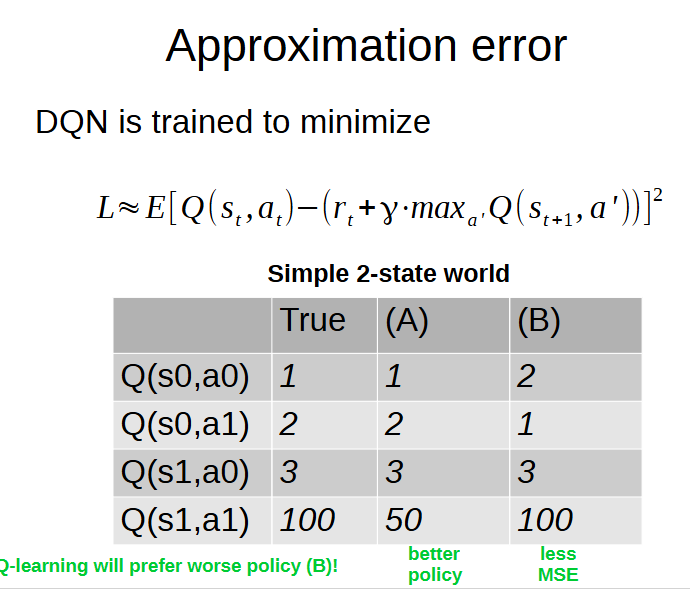
\includegraphics[width=0.85\textwidth]{figures/lecture10_q_approximation_error.png}
    \caption{Approximation error: хорошее приближение \(Q\)-values по MSE не всегда даёт хорошую policy.}
\end{figure}

\subsection{Policy-based подход}

В policy-based методах мы не обязаны учить \(Q(s,a)\). Вместо этого policy задаётся напрямую:

\[
\pi_\theta(a \mid s).
\]

Тогда агент сразу учится выбирать действия.

Идея:

\[
s
\longrightarrow
\pi_\theta(\cdot \mid s)
\longrightarrow
a.
\]

Преимущества policy-based подхода:

\begin{itemize}
    \item решает более прямую задачу: учит policy, а не value function;
    \item естественно поддерживает stochastic policies;
    \item stochastic policy сама обеспечивает exploration;
    \item удобно работает с continuous action spaces;
    \item можно оптимизировать expected return напрямую.
\end{itemize}

\subsection{Deterministic и stochastic policies}

Существуют два основных типа policies.

\subsubsection{Deterministic policy}

Детерминированная policy всегда выбирает одно действие в данном состоянии:

\[
a = \pi_\theta(s).
\]

То есть если агент снова попадёт в то же состояние, он выберет то же действие.

\subsubsection{Stochastic policy}

Стохастическая policy задаёт распределение по действиям:

\[
a \sim \pi_\theta(a \mid s).
\]

То есть действие сэмплируется из распределения.

Например, для дискретного action space policy может быть categorical distribution:

\[
\pi_\theta(a \mid s)
=
\operatorname{Categorical}(p_1,\dots,p_K).
\]

Для continuous action space policy может быть нормальным распределением:

\[
\pi_\theta(a \mid s)
=
\mathcal{N}(\mu_\theta(s), \sigma_\theta^2(s)).
\]

\subsection{Когда stochastic policy полезна}

Stochastic policy особенно полезна, когда оптимальная стратегия не должна быть детерминированной.

Классический пример:

\[
\text{rock-paper-scissors}.
\]

Если всегда играть один и тот же ход, противник быстро адаптируется. Оптимальная стратегия должна случайно выбирать между действиями.

Также stochastic policy полезна для exploration: агент может пробовать разные действия без дополнительной \(\varepsilon\)-greedy схемы.

\subsection{Value-based vs policy-based}

\begin{table}[H]
\centering
\begin{tabular}{p{0.45\textwidth} p{0.45\textwidth}}
\toprule
\textbf{Value-based} & \textbf{Policy-based} \\
\midrule

Учит \(Q_\theta(s,a)\) или \(V_\theta(s)\). &
Учит policy \(\pi_\theta(a\mid s)\) напрямую. \\

Policy выводится через:
\[
a=\arg\max_a Q_\theta(s,a).
\]
&
Policy уже является выходом модели. \\

Exploration обычно добавляется искусственно:
\(\varepsilon\)-greedy, softmax. &
Exploration естественно возникает из stochastic policy. \\

Хорошо использует partial experience через TD. &
Классический REINFORCE использует полные trajectories. \\

Может быть сложнее для continuous actions. &
Хорошо подходит для continuous action spaces. \\

\bottomrule
\end{tabular}
\caption{Сравнение value-based и policy-based подходов.}
\end{table}

% Слайд 47. Value-based vs policy-based: различия между Q-learning/SARSA/MCTS и REINFORCE/CEM.
\begin{figure}[H]
    \centering
    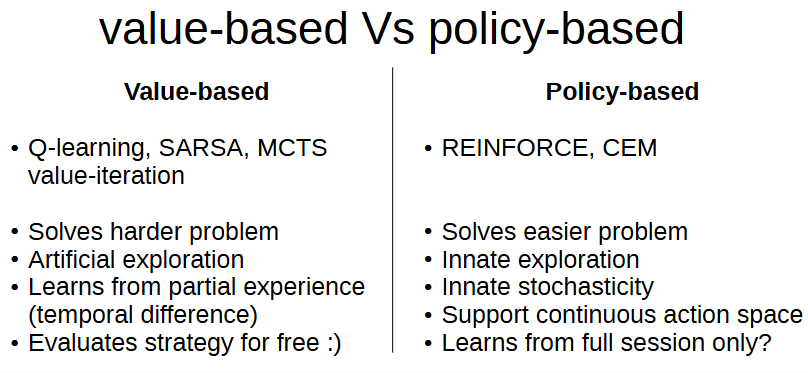
\includegraphics[width=0.85\textwidth]{figures/lecture10_value_based_vs_policy_based.png}
    \caption{Value-based методы учат value function, policy-based методы напрямую учат policy.}
\end{figure}

\subsection{Cross-Entropy Method как policy-based метод}

Cross-Entropy Method также можно рассматривать как policy-based подход.

Пусть policy параметризована нейросетью:

\[
\pi_\theta(a \mid s).
\]

CEM работает так:

\begin{enumerate}
    \item инициализировать параметры:
    \[
    \theta_0 \leftarrow random;
    \]

    \item сэмплировать \(N\) sessions текущей policy;

    \item выбрать \(M\) лучших sessions, то есть elite sessions;

    \item обновить policy так, чтобы увеличить вероятность elite actions:
    \[
    \theta_{i+1}
    =
    \theta_i
    +
    \alpha
    \nabla
    \sum_i
    \log \pi_{\theta_i}(a_i \mid s_i)
    \cdot
    \mathbb{I}[(s_i,a_i)\in Elite].
    \]
\end{enumerate}

CEM не учит \(Q(s,a)\), а напрямую увеличивает вероятность хороших действий.

\subsection{Policy Gradient: основная идея}

В policy gradient мы хотим напрямую максимизировать expected return:

\[
J(\theta)
=
\mathbb{E}_{\tau \sim \pi_\theta}
[
G(\tau)
].
\]

Здесь:

\begin{itemize}
    \item \(\theta\) --- параметры policy;
    \item \(\tau\) --- trajectory;
    \item \(G(\tau)\) --- return trajectory.
\end{itemize}

Идея:

\[
\theta
\leftarrow
\theta
+
\alpha \nabla_\theta J(\theta).
\]

То есть мы хотим двигать параметры policy в направлении увеличения expected return.

\subsection{Objective для one-step process}

Для простоты рассмотрим one-step процесс.

Состояние:

\[
s \sim p(s).
\]

Действие:

\[
a \sim \pi_\theta(a \mid s).
\]

Reward:

\[
R(s,a).
\]

Objective:

\[
J(\theta)
=
\mathbb{E}_{s\sim p(s), a\sim \pi_\theta(a\mid s)}
[
R(s,a)
].
\]

В интегральной форме:

\[
J(\theta)
=
\int_s
p(s)
\int_a
\pi_\theta(a\mid s)
R(s,a)
\,da\,ds.
\]

Проблема: мы хотим вычислить \(\nabla_\theta J(\theta)\), но reward и среда могут быть недифференцируемыми.

\subsection{Почему обычный gradient сложен}

Если просто сэмплировать \(N\) trajectories и оценить:

\[
J(\theta)
\approx
\frac{1}{N}
\sum_{i=1}^{N}
R(s_i,a_i),
\]

то неочевидно, как дифференцировать это по \(\theta\), потому что действие \(a_i\) было сэмплировано из policy.

Параметры \(\theta\) сидят внутри распределения:

\[
\pi_\theta(a\mid s).
\]

Нужно получить аналитическую формулу gradient, которая позволяет использовать sampled actions.

\subsection{Log-derivative trick}

Ключевой трюк:

\[
\nabla_\theta \log \pi_\theta(z)
=
\frac{1}{\pi_\theta(z)}
\nabla_\theta \pi_\theta(z).
\]

Отсюда:

\[
\nabla_\theta \pi_\theta(z)
=
\pi_\theta(z)
\nabla_\theta \log \pi_\theta(z).
\]

Это называется:

\[
\text{log-derivative trick}
\]

или

\[
\text{score function trick}.
\]

Он позволяет переписать gradient expectation так, чтобы снова получить expectation, который можно оценивать sampling-ом.

\subsection{Policy gradient derivation}

Начинаем с objective:

\[
J(\theta)
=
\int_s
p(s)
\int_a
\pi_\theta(a\mid s)
R(s,a)
\,da\,ds.
\]

Gradient:

\[
\nabla_\theta J(\theta)
=
\int_s
p(s)
\int_a
\nabla_\theta \pi_\theta(a\mid s)
R(s,a)
\,da\,ds.
\]

Применяем log-derivative trick:

\[
\nabla_\theta \pi_\theta(a\mid s)
=
\pi_\theta(a\mid s)
\nabla_\theta
\log \pi_\theta(a\mid s).
\]

Тогда:

\[
\nabla_\theta J(\theta)
=
\int_s
p(s)
\int_a
\pi_\theta(a\mid s)
\nabla_\theta
\log \pi_\theta(a\mid s)
R(s,a)
\,da\,ds.
\]

Это expectation:

\[
\nabla_\theta J(\theta)
=
\mathbb{E}_{s\sim p(s), a\sim \pi_\theta(a\mid s)}
[
\nabla_\theta \log \pi_\theta(a\mid s) R(s,a)
].
\]

\subsection{REINFORCE для bandit setting}

Для one-step или bandit setting:

\[
\nabla_\theta J(\theta)
=
\mathbb{E}
[
\nabla_\theta
\log \pi_\theta(a\mid s)
R(s,a)
].
\]

Оценка по samples:

\[
\nabla_\theta J(\theta)
\approx
\frac{1}{N}
\sum_{i=1}^{N}
\nabla_\theta
\log \pi_\theta(a_i\mid s_i)
R(s_i,a_i).
\]

Алгоритм:

\begin{enumerate}
    \item инициализировать policy parameters:
    \[
    \theta_0 \leftarrow random;
    \]

    \item сэмплировать \(N\) sessions под текущей policy \(\pi_\theta\);

    \item оценить policy gradient;

    \item обновить параметры:
    \[
    \theta_{i+1}
    =
    \theta_i
    +
    \alpha \nabla_\theta J.
    \]
\end{enumerate}

\subsection{Policy gradient для discounted reward}

В многошаговой задаче вместо immediate reward используется action-value function:

\[
Q^\pi(s,a)
=
\mathbb{E}[G_t \mid S_t=s, A_t=a].
\]

Policy gradient:

\[
\nabla_\theta J(\theta)
=
\mathbb{E}_{s\sim p(s), a\sim \pi_\theta(a\mid s)}
[
\nabla_\theta
\log \pi_\theta(a\mid s)
Q^\pi(s,a)
].
\]

Интуиция:

\begin{itemize}
    \item если действие \(a\) в состоянии \(s\) привело к большому \(Q^\pi(s,a)\), нужно увеличить \(\log \pi_\theta(a\mid s)\);
    \item если действие плохое, его вероятность нужно уменьшить.
\end{itemize}

\subsection{REINFORCE algorithm}

В REINFORCE \(Q^\pi(s,a)\) оценивается через sampled return:

\[
G_t
=
r_t
+
\gamma r_{t+1}
+
\gamma^2 r_{t+2}
+
\dots
\]

Так как:

\[
Q^\pi(s_t,a_t)
=
\mathbb{E}[G_t \mid s_t,a_t],
\]

можно использовать \(G_t\) как sample estimate для \(Q^\pi(s_t,a_t)\).

Тогда gradient estimate:

\[
\nabla_\theta J
\approx
\frac{1}{N}
\sum_{i=1}^{N}
\sum_{(s_t,a_t)\in \tau_i}
\nabla_\theta
\log \pi_\theta(a_t\mid s_t)
G_t.
\]

% Слайд 42. REINFORCE: Q(s,a) оценивается через sampled return G_t.
\begin{figure}[H]
    \centering
    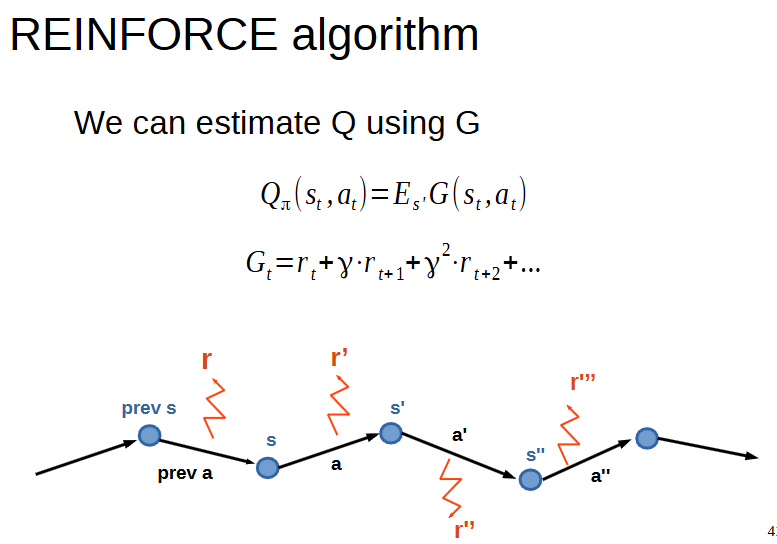
\includegraphics[width=0.85\textwidth]{figures/lecture10_reinforce_q_using_g.png}
    \caption{REINFORCE оценивает \(Q^\pi(s,a)\) через return \(G_t\), посчитанный по sampled trajectory.}
\end{figure}

\subsection{Вычисление discounted returns}

Return можно считать рекурсивно:

\[
G_t
=
r_t
+
\gamma r_{t+1}
+
\gamma^2 r_{t+2}
+
\dots
\]

\[
G_t
=
r_t
+
\gamma
(
r_{t+1}
+
\gamma r_{t+2}
+
\dots
).
\]

То есть:

\[
G_t
=
r_t + \gamma G_{t+1}.
\]

Благодаря этому все \(G_t\) для trajectory можно посчитать за линейное время, проходя с конца эпизода к началу.

% Слайд 43. Discounted rewards: G_t = r_t + gamma G_{t+1}, все G считаются за linear time.
\begin{figure}[H]
    \centering
    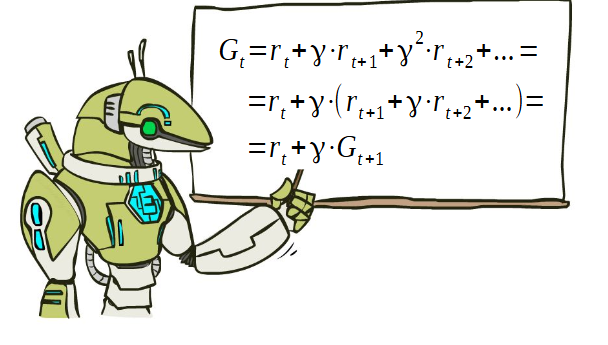
\includegraphics[width=0.8\textwidth]{figures/lecture10_discounted_returns_linear_time.png}
    \caption{Рекурсивная формула \(G_t=r_t+\gamma G_{t+1}\) позволяет посчитать returns за линейное время.}
\end{figure}

\subsection{REINFORCE является on-policy}

REINFORCE сэмплирует trajectories из текущей policy:

\[
\tau_i \sim \pi_\theta.
\]

Затем gradient оценивается по actions, выбранным этой же policy.

Поэтому REINFORCE является \textbf{on-policy} алгоритмом.

Это означает, что после обновления policy старые trajectories становятся менее корректными для обучения новой policy.

\subsection{Интуиция policy gradient}

Формула:

\[
\nabla_\theta J
\approx
\sum_t
\nabla_\theta \log \pi_\theta(a_t\mid s_t)G_t
\]

имеет простую интерпретацию.

Если \(G_t\) большой:

\[
\text{увеличиваем вероятность } a_t \text{ в } s_t.
\]

Если \(G_t\) маленький или отрицательный:

\[
\text{уменьшаем вероятность } a_t \text{ в } s_t.
\]

Множитель

\[
\nabla_\theta \log \pi_\theta(a_t\mid s_t)
\]

указывает, как изменить параметры, чтобы увеличить вероятность выбранного действия.

\subsection{Проблема высокой дисперсии}

REINFORCE может иметь высокую дисперсию.

Причина: \(G_t\) зависит от всей последующей trajectory и может сильно шуметь.

Например, действие в хорошем состоянии может получить плохой return из-за неудачных будущих случайностей. Или хорошее действие в плохом состоянии может выглядеть хуже, чем оно есть.

Нужно уменьшать variance gradient estimate.

Один из главных способов:

\[
\text{baseline}.
\]

\subsection{Baselines в REINFORCE}

В policy gradient можно вычитать baseline \(b(s)\), не зависящий от действия:

\[
\nabla_\theta J
=
\mathbb{E}
[
\nabla_\theta
\log \pi_\theta(a\mid s)
(Q(s,a)-b(s))
].
\]

Такой baseline не меняет математическое ожидание gradient.

Почему?

Второй член:

\[
\mathbb{E}_{a\sim\pi_\theta}
[
\nabla_\theta
\log \pi_\theta(a\mid s)b(s)
]
\]

равен:

\[
b(s)
\mathbb{E}_{a\sim\pi_\theta}
[
\nabla_\theta
\log \pi_\theta(a\mid s)
].
\]

А:

\[
\mathbb{E}_{a\sim\pi_\theta}
[
\nabla_\theta
\log \pi_\theta(a\mid s)
]
=
\sum_a
\pi_\theta(a\mid s)
\nabla_\theta
\log \pi_\theta(a\mid s)
\]

\[
=
\sum_a
\nabla_\theta
\pi_\theta(a\mid s)
=
\nabla_\theta
\sum_a
\pi_\theta(a\mid s)
=
\nabla_\theta 1
=
0.
\]

Значит baseline не меняет direction of expected gradient.

\subsection{Зачем нужен baseline}

Хотя baseline не меняет expected gradient, он может уменьшить дисперсию.

Gradient variance зависит от:

\[
\operatorname{Var}[Q(s,a)-b(s)].
\]

Если \(b(s)\) коррелирует с \(Q(s,a)\), variance уменьшается.

Наивный baseline:

\[
b = \text{moving average of } Q.
\]

Более сильный baseline:

\[
b(s)=V(s).
\]

Тогда:

\[
Q(s,a)-V(s)
\]

называется advantage.

\subsection{Advantage function}

\textbf{Advantage} показывает, насколько действие \(a\) лучше среднего действия в состоянии \(s\):

\[
A(s,a)
=
Q(s,a)-V(s).
\]

Интерпретация:

\begin{itemize}
    \item \(A(s,a)>0\): действие лучше среднего для этого состояния;
    \item \(A(s,a)<0\): действие хуже среднего;
    \item \(A(s,a)=0\): действие примерно соответствует среднему уровню состояния.
\end{itemize}

Policy gradient с advantage:

\[
\nabla_\theta J
\approx
\frac{1}{N}
\sum_i
\sum_{s,a\in \tau_i}
\nabla_\theta
\log \pi_\theta(a\mid s)
A(s,a).
\]

\subsection{Actor-Critic}

\textbf{Actor-Critic} объединяет policy-based и value-based подходы.

Есть две части:

\begin{itemize}
    \item \textbf{actor} --- policy:
    \[
    \pi_\theta(a\mid s);
    \]

    \item \textbf{critic} --- value function:
    \[
    V_w(s)
    \]
    или
    \[
    Q_w(s,a).
    \]
\end{itemize}

Actor выбирает действия, critic оценивает, насколько они хороши.

% Слайд 60. Actor-critic: учим одновременно V(s) и pi(a|s).
\begin{figure}[H]
    \centering
    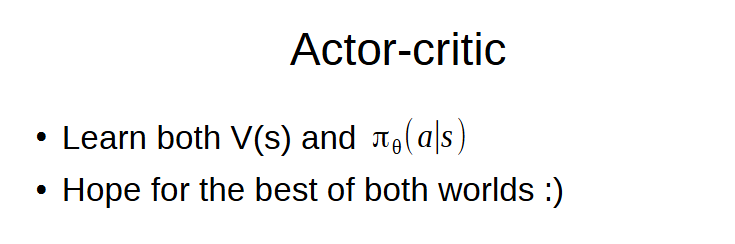
\includegraphics[width=0.8\textwidth]{figures/lecture10_actor_critic.png}
    \caption{Actor-Critic: actor учит policy, critic учит value function.}
\end{figure}

\subsection{Advantage Actor-Critic}

В Advantage Actor-Critic используется:

\[
A(s,a)=Q(s,a)-V(s).
\]

Но \(Q(s,a)\) можно приблизить через one-step bootstrap:

\[
Q(s,a)
\approx
r+\gamma V(s').
\]

Тогда:

\[
A(s,a)
\approx
r+\gamma V(s')-V(s).
\]

Это также похоже на temporal difference error:

\[
\delta_t
=
r_t+\gamma V(s_{t+1})-V(s_t).
\]

Actor update:

\[
\nabla_\theta J_{actor}
\approx
\frac{1}{N}
\sum_i
\sum_{s,a\in \tau_i}
\nabla_\theta
\log \pi_\theta(a\mid s)
A(s,a).
\]

Critic обучается минимизировать ошибку value prediction:

\[
L_{critic}
\approx
\frac{1}{N}
\sum_i
\sum_{s,a\in \tau_i}
\left(
V_w(s)
-
[
r+\gamma V_w(s')
]
\right)^2.
\]

\subsection{Continuous action spaces}

Policy gradient методы естественно работают с continuous action spaces.

Если действий бесконечно много, не нужно брать:

\[
\arg\max_a Q(s,a)
\]

по непрерывному множеству.

Можно просто задать policy distribution, например:

\[
\pi_\theta(a\mid s)
=
\mathcal{N}
(
\mu_\theta(s),
\sigma_\theta^2(s)
).
\]

А затем сэмплировать:

\[
a \sim \pi_\theta(a\mid s).
\]

Алгоритм почти не меняется: нужно только уметь считать

\[
\log \pi_\theta(a\mid s)
\]

и его gradient.

\subsection{Entropy regularization}

В policy gradient методах policy может слишком быстро стать почти детерминированной. Тогда exploration ухудшается.

Чтобы предотвратить premature convergence, добавляют entropy regularization.

Entropy policy:

\[
H(\pi(\cdot\mid s))
=
-
\sum_a
\pi(a\mid s)
\log \pi(a\mid s).
\]

К objective можно добавить:

\[
J'(\theta)
=
J(\theta)
+
\beta
\mathbb{E}_s
[
H(\pi_\theta(\cdot\mid s))
].
\]

Это поощряет более случайную policy и поддерживает exploration.

\subsection{A3C}

\textbf{A3C} расшифровывается как:

\[
\text{Asynchronous Advantage Actor-Critic}.
\]

Основные идеи:

\begin{itemize}
    \item parallel game sessions;
    \item async multi-CPU training;
    \item no experience replay;
    \item LSTM policy;
    \item n-step advantage.
\end{itemize}

Несколько worker-ов параллельно взаимодействуют со своими копиями среды и обновляют global network.

% Слайд 68. A3C: несколько workers параллельно собирают experience и обновляют global network.
\begin{figure}[H]
    \centering
    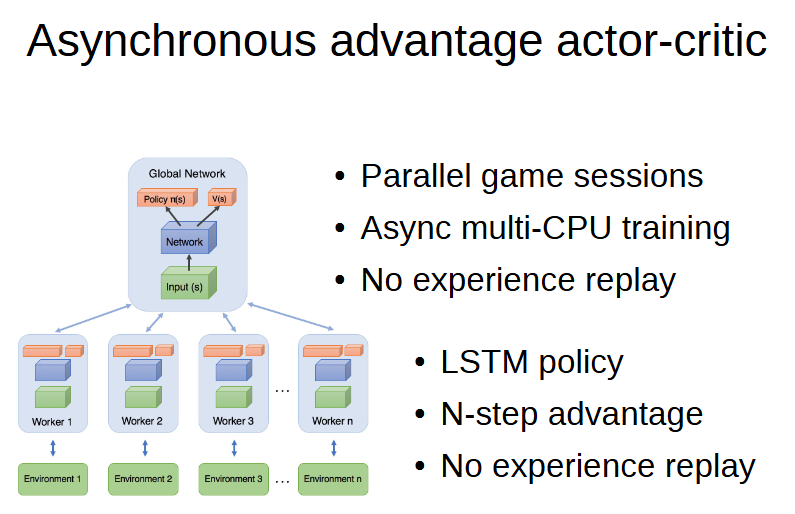
\includegraphics[width=0.85\textwidth]{figures/lecture10_a3c_scheme.png}
    \caption{A3C использует параллельные sessions и asynchronous updates.}
\end{figure}

\subsection{IMPALA}

\textbf{IMPALA} --- масштабируемая actor-critic архитектура.

Ключевые идеи:

\begin{itemize}
    \item massively parallel training;
    \item separate actor and learner processes;
    \item небольшой experience replay;
    \item importance sampling для коррекции различий между policy акторов и learner-а.
\end{itemize}

IMPALA отделяет сбор опыта от обучения модели, что позволяет масштабировать RL на большое число сред.

\subsection{Практические замечания}

В лекции выделяются несколько практических советов:

\begin{itemize}
    \item ошибки \(V(s)\) менее критичны, чем ошибки \(Q(s,a)\) в Q-learning: actor всё ещё может учиться, даже если critic пока слабый;
    \item полезно регуляризовать policy entropy, чтобы избежать ранней потери exploration;
    \item можно обучаться на parallel sessions;
    \item для численной стабильности удобно использовать \texttt{logsoftmax}.
\end{itemize}

\subsection{Главные выводы}

\begin{itemize}
    \item Value-based методы учат \(Q\)-function, а policy потом получается через \(\arg\max\).
    \item Иногда учить точные \(Q\)-values сложнее, чем напрямую учить policy.
    \item Policy-based методы напрямую параметризуют:
    \[
    \pi_\theta(a\mid s).
    \]

    \item Policy gradient максимизирует expected return:
    \[
    J(\theta)=\mathbb{E}_{\tau\sim\pi_\theta}[G(\tau)].
    \]

    \item Log-derivative trick:
    \[
    \nabla_\theta \pi_\theta(z)
    =
    \pi_\theta(z)\nabla_\theta\log\pi_\theta(z).
    \]

    \item REINFORCE использует gradient:
    \[
    \nabla_\theta J
    \approx
    \sum_t
    \nabla_\theta
    \log \pi_\theta(a_t\mid s_t)G_t.
    \]

    \item REINFORCE является on-policy.
    \item Baseline \(b(s)\) не меняет expected gradient, но может уменьшить variance.
    \item Advantage:
    \[
    A(s,a)=Q(s,a)-V(s).
    \]

    \item Actor-critic учит одновременно policy и value function.
    \item Advantage actor-critic использует:
    \[
    A(s,a)\approx r+\gamma V(s')-V(s).
    \]

    \item Policy gradient естественно работает с continuous action spaces.
\end{itemize}

\subsection{Что важно помнить к экзамену}

\begin{enumerate}
    \item Value-based policy:
    \[
    \pi(s)=\arg\max_a Q_\theta(s,a).
    \]

    \item Policy-based model:
    \[
    \pi_\theta(a\mid s).
    \]

    \item Deterministic policy:
    \[
    a=\pi_\theta(s).
    \]

    \item Stochastic policy:
    \[
    a\sim\pi_\theta(a\mid s).
    \]

    \item Policy gradient objective:
    \[
    J(\theta)
    =
    \mathbb{E}_{\tau\sim\pi_\theta}
    [
    G(\tau)
    ].
    \]

    \item Log-derivative trick:
    \[
    \nabla_\theta\log\pi_\theta(z)
    =
    \frac{1}{\pi_\theta(z)}
    \nabla_\theta\pi_\theta(z).
    \]

    \item Policy gradient:
    \[
    \nabla_\theta J
    =
    \mathbb{E}
    [
    \nabla_\theta
    \log \pi_\theta(a\mid s)
    Q^\pi(s,a)
    ].
    \]

    \item REINFORCE estimate:
    \[
    \nabla_\theta J
    \approx
    \frac{1}{N}
    \sum_{i=1}^{N}
    \sum_{t}
    \nabla_\theta
    \log \pi_\theta(a_t^i\mid s_t^i)
    G_t^i.
    \]

    \item Discounted return:
    \[
    G_t=r_t+\gamma G_{t+1}.
    \]

    \item Baseline:
    \[
    \nabla_\theta J
    =
    \mathbb{E}
    [
    \nabla_\theta
    \log \pi_\theta(a\mid s)
    (Q(s,a)-b(s))
    ].
    \]

    \item Baseline не должен зависеть от action \(a\).

    \item Advantage:
    \[
    A(s,a)=Q(s,a)-V(s).
    \]

    \item One-step advantage estimate:
    \[
    A(s,a)\approx r+\gamma V(s')-V(s).
    \]

    \item Actor loss direction:
    \[
    \nabla_\theta J_{actor}
    \approx
    \sum_t
    \nabla_\theta
    \log \pi_\theta(a_t\mid s_t)
    A(s_t,a_t).
    \]

    \item Critic loss:
    \[
    L_{critic}
    \approx
    \sum_t
    \left(
    V_w(s_t)
    -
    [
    r_t+\gamma V_w(s_{t+1})
    ]
    \right)^2.
    \]

    \item Continuous actions:
    \[
    \pi_\theta(a\mid s)
    =
    \mathcal{N}(\mu_\theta(s),\sigma_\theta^2(s)).
    \]

    \item A3C:
    \[
    \text{Asynchronous Advantage Actor-Critic}.
    \]
\end{enumerate}
```


```latex
\section{Лекция 11. Reinforcement Learning in Language Modeling and SCST}

\subsection{План лекции}

В этой лекции рассматриваются:

\begin{itemize}
    \item общая RL-постановка для sequence generation;
    \item encoder-decoder задачи;
    \item supervised seq2seq learning;
    \item проблемы distribution shift;
    \item неоднозначность правильных ответов в machine translation;
    \item применение RL к seq2seq;
    \item seq2seq как POMDP;
    \item policy gradient для генерации текста;
    \item supervised learning vs policy gradient;
    \item training vs inference mismatch;
    \item self-critical sequence training;
    \item image captioning with SCST;
    \item discrete GANs как бонусная тема.
\end{itemize}

Главная идея лекции: генерацию текста можно рассматривать как задачу Reinforcement Learning, где policy --- это decoder, action --- следующий токен, а reward --- внешняя метрика качества вроде BLEU, CIDEr или domain-specific reward. Это позволяет оптимизировать не likelihood reference-последовательности, а непосредственно целевую метрику.

\subsection{Общий RL-формализм}

В общем виде задача RL записывается как максимизация expected reward по policy:

\[
J
=
\mathbb{E}_{s \sim d(s), \, a \sim \pi(a \mid obs(s))}
[
R(s,a)
].
\]

Здесь:

\begin{itemize}
    \item \(s\) --- состояние среды;
    \item \(obs(s)\) --- наблюдение агента;
    \item \(a\) --- действие;
    \item \(\pi(a \mid obs(s))\) --- policy;
    \item \(R(s,a)\) --- reward.
\end{itemize}

Reward может быть black-box функцией. Например, в sequence generation он может быть внешней метрикой качества:

\[
R(x,y) = BLEU(y, y_{ref}),
\]

или

\[
R(x,y) = CIDEr(y, y_{ref}).
\]

В частном случае можно использовать discounted return:

\[
G(s,a)
=
r(s,a)
+
\gamma G(s',a').
\]

Markov property:

\[
P(s' \mid s,a,*) = P(s'\mid s,a).
\]

Если наблюдение полностью описывает состояние, то:

\[
obs(s)=s.
\]

Но в seq2seq-задачах часто удобнее говорить о частично наблюдаемой задаче, потому что decoder видит только вход и уже сгенерированные токены, а не всю скрытую структуру правильного ответа.

\subsection{Общие подходы к оптимизации policy}

Для оптимизации policy можно использовать разные подходы:

\begin{itemize}
    \item \textbf{Evolution strategies}: немного изменять policy, запускать её и оставлять варианты с большим \(J\).
    \item \textbf{Value-based methods}: оценивать \(J\) или \(Q(s,a)\) как функцию действия и выбирать лучшее действие.
    \item \textbf{Policy gradient}: напрямую подниматься по градиенту \(\nabla J\) относительно параметров policy.
    \item \textbf{Bayesian optimization}: строить surrogate model для \(J\) и выбирать наиболее информативные policy.
    \item \textbf{Simulated annealing}.
    \item \textbf{Cross-Entropy Method}.
\end{itemize}

В этой лекции основной акцент сделан на policy gradient для sequence generation.

\subsection{Encoder-decoder architectures}

Encoder-decoder архитектуры решают задачи вида:

\[
x \rightarrow y,
\]

где вход \(x\) может быть последовательностью или произвольным объектом, а выход \(y\) --- последовательность.

Encoder читает input data, decoder генерирует output sequence.

Примеры задач:

\begin{itemize}
    \item machine translation;
    \item image captioning;
    \item speech recognition или word-to-transcript;
    \item conversation systems;
    \item image to LaTeX;
    \item code to docstring.
\end{itemize}

% Слайд 7. Encoder-decoder tasks: machine translation, image captioning, conversation, image-to-latex, code-to-docstring.
\begin{figure}[H]
    \centering
    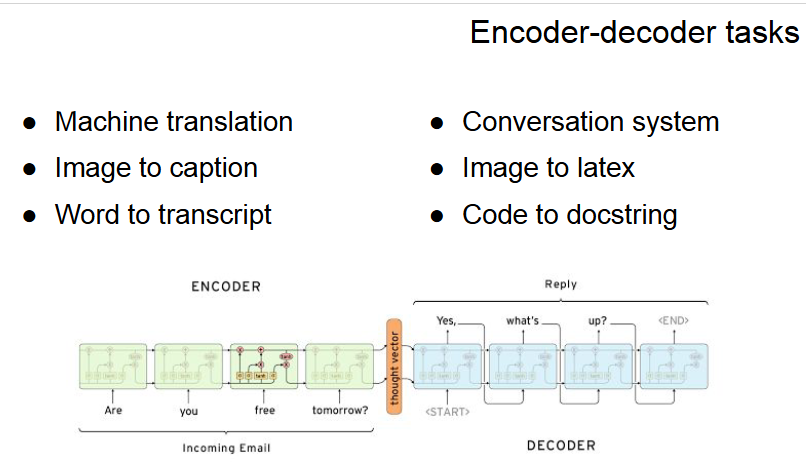
\includegraphics[width=0.85\textwidth]{figures/lecture11_encoder_decoder_tasks.png}
    \caption{Encoder-decoder задачи: один объект или последовательность преобразуется в выходную последовательность.}
\end{figure}

\subsection{Supervised seq2seq learning}

В supervised seq2seq learning есть датасет пар:

\[
(x,y),
\]

где:

\begin{itemize}
    \item \(x\) --- вход;
    \item \(y\) --- reference output.
\end{itemize}

Например, в machine translation:

\[
x = \text{sentence in Chinese},
\]

\[
y = \text{sentence in English}.
\]

Обычная supervised objective:

\[
\max_\theta \log P_\theta(y \mid x).
\]

Для sequence output:

\[
P_\theta(y \mid x)
=
\prod_{t=1}^{T}
P_\theta(y_t \mid x, y_{<t}).
\]

Тогда negative log-likelihood loss:

\[
\mathcal{L}_{CE}
=
-
\sum_{t=1}^{T}
\log P_\theta(y_t \mid x, y_{<t}).
\]

Это teacher forcing: во время обучения decoder получает правильные предыдущие токены \(y_{<t}\).

\subsection{Примеры supervised seq2seq задач}

\subsubsection{Machine translation}

Постановка:

\begin{itemize}
    \item прочитать предложение на исходном языке;
    \item сгенерировать предложение на целевом языке;
    \item предложения должны иметь одинаковый смысл.
\end{itemize}

Supervised solution:

\[
\max_\theta \log P_\theta(\text{translation}\mid \text{source}).
\]

\subsubsection{Conversation systems}

Постановка:

\begin{itemize}
    \item прочитать фразу пользователя;
    \item сгенерировать ответ;
    \item система должна поддерживать диалог.
\end{itemize}

Supervised solution:

\[
\max_\theta \log P_\theta(\text{response}\mid \text{phrase}).
\]

\subsubsection{Grapheme to phoneme}

Постановка:

\begin{itemize}
    \item прочитать слово как последовательность символов;
    \item сгенерировать транскрипцию как последовательность фонем.
\end{itemize}

Например:

\[
\text{hedgehog}
\rightarrow
\text{phoneme sequence}.
\]

Supervised solution:

\[
\max_\theta \log P_\theta(\text{transcript}\mid \text{word}).
\]

\subsection{Attentive translation}

В attentive translation decoder на каждом шаге сам выбирает, на какие hidden states encoder-а смотреть.

То есть decoder не обязан использовать только один финальный encoder state. Вместо этого он получает weighted combination encoder states.

Attention одновременно помогает учить:

\begin{itemize}
    \item word alignment;
    \item word translation.
\end{itemize}

% Слайд 11. Attentive translation: attention matrix показывает alignment между source и target словами.
\begin{figure}[H]
    \centering
    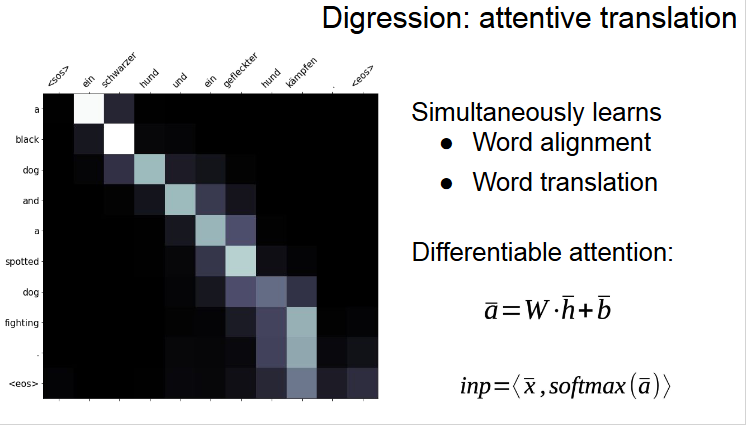
\includegraphics[width=0.85\textwidth]{figures/lecture11_attentive_translation_alignment.png}
    \caption{Attention в машинном переводе одновременно учит word alignment и translation.}
\end{figure}

\subsection{Обобщённая постановка sequence generation}

Многие задачи можно записать в общем виде:

\[
x \sim X,
\]

\[
y \sim Y.
\]

Нужно произвести ответ:

\[
y^*
=
\arg\max_y R(x,y).
\]

Здесь \(R(x,y)\) --- метрика качества ответа.

Обычное supervised решение:

\begin{itemize}
    \item взять датасет хороших пар \((x,y)\);
    \item максимизировать:
    \[
    \log P_\theta(y\mid x).
    \]
\end{itemize}

Этот подход хорошо работает, если данные:

\begin{itemize}
    \item многочисленные;
    \item качественные;
    \item близкие к оптимальным по \(R(x,y)\).
\end{itemize}

Проблема: часто эти условия не выполняются.

\subsection{Distribution shift}

В supervised seq2seq есть важное расхождение между training и inference.

Во время обучения модель предсказывает:

\[
P_\theta(y_{t+1} \mid x, y_{0:t}),
\]

где:

\[
y_{0:t} \sim reference.
\]

То есть предыдущие токены взяты из правильного ответа.

Во время inference модель предсказывает:

\[
P_\theta(y_{t+1} \mid x, \hat{y}_{0:t}),
\]

где:

\[
\hat{y}_{0:t} \sim model.
\]

Если модель на каком-то шаге ошиблась, следующий hidden state оказывается в области, которую модель почти не видела при обучении. Ошибка может усиливаться на следующих шагах.

Это называется:

\[
\text{distribution shift}.
\]

% Слайд 18. Distribution shift: при обучении decoder видит reference-prefix, а при inference — model-generated prefix.
\begin{figure}[H]
    \centering
    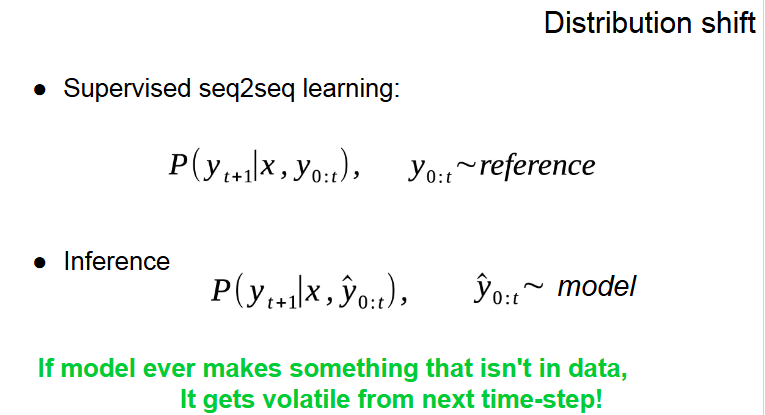
\includegraphics[width=0.85\textwidth]{figures/lecture11_distribution_shift.png}
    \caption{Distribution shift в seq2seq: training использует reference prefix, inference использует generated prefix.}
\end{figure}

\subsection{Проблема неоднозначности правильного ответа}

В machine translation часто существует много корректных переводов одного и того же source sentence.

Например, один source sentence может иметь варианты:

\begin{itemize}
    \item ``I'm searching for some gifts for my family.''
    \item ``I want to find something for my family as presents.''
    \item ``I'm about to buy some presents for my family.''
    \item ``I'd like to buy my family something as a gift.''
    \item ``I'm looking for a present for my family.''
\end{itemize}

Supervised maximum likelihood заставляет модель поднимать вероятность конкретных reference translations. Но модели не обязательно нужно выучить все возможные правильные переводы. Ей достаточно генерировать хотя бы один хороший.

Проблема likelihood: модель может иметь хороший mean log probability на reference data, но при этом давать много плохих outputs вне датасета.

\subsection{Проблемы conversation systems}

Для диалоговых систем есть два типа данных:

\begin{itemize}
    \item большие сырые данные;
    \item маленькие чистые данные.
\end{itemize}

Большие сырые данные:

\begin{itemize}
    \item Twitter, subtitles, books, logs;
    \item \(10^6\)--\(10^8\) samples;
    \item достаточно большие;
    \item но могут иметь suboptimal \(R(x,y)\).
\end{itemize}

Маленькие чистые данные:

\begin{itemize}
    \item moderated logs;
    \item assessor-written conversations;
    \item \(10^2\)--\(10^4\) samples;
    \item ответы ближе к оптимальным;
    \item но данных мало.
\end{itemize}

Если обучить банковского Q\&A-бота на сырых социальных данных, он может выучить нежелательное поведение. Классическая проблема: модель оптимизирует статистику датасета, а не бизнес-цель и не безопасность.

\subsection{Seq2seq как POMDP}

Sequence generation можно рассматривать как частично наблюдаемый MDP.

Для seq2seq:

\begin{itemize}
    \item hidden state \(s\) --- состояние перевода или диалога;
    \item initial state \(s_0\) --- encoder output;
    \item observation \(o_t\) --- предыдущие сгенерированные слова;
    \item action \(a_t\) --- написать следующий токен;
    \item reward \(r\) --- domain-specific reward, например BLEU.
\end{itemize}

То есть decoder policy:

\[
\pi_\theta(a_t \mid obs(s_t))
\]

выбирает следующий токен.

Полная последовательность действий:

\[
a_1, a_2, \dots, a_T
\]

образует generated output.

Reward может начисляться в конце всей последовательности:

\[
R(x, \hat{y}).
\]

% Слайд 29. Seq2seq as POMDP: action = write next word, reward = BLEU/domain-specific metric.
\begin{figure}[H]
    \centering
    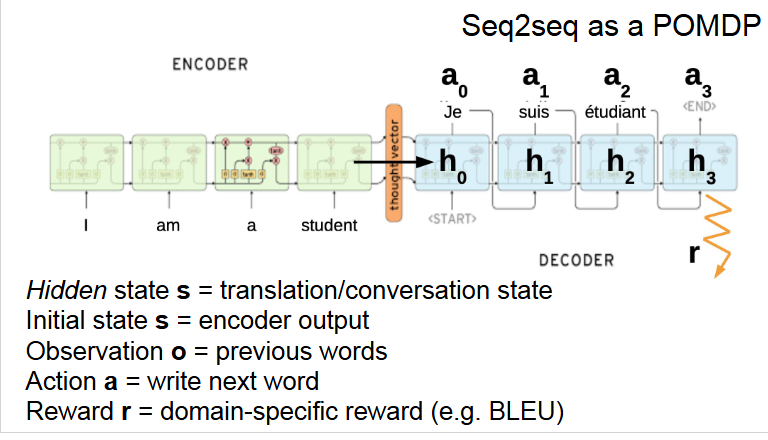
\includegraphics[width=0.85\textwidth]{figures/lecture11_seq2seq_as_pomdp.png}
    \caption{Seq2seq можно рассматривать как POMDP: decoder выбирает следующий токен как действие.}
\end{figure}

\subsection{Policy Gradient для sequence generation}

Пусть objective:

\[
J(\theta)
=
\mathbb{E}_{s\sim p(s), \, a\sim\pi_\theta(a\mid s)}
[
R(s,a)
].
\]

В seq2seq случае \(a\) можно понимать как всю сгенерированную последовательность:

\[
a = \hat{y}.
\]

Reward:

\[
R(s,a)
\]

может быть BLEU, CIDEr, пользовательская оценка или другой black-box score.

Наивная Monte Carlo оценка:

\[
J(\theta)
\approx
\frac{1}{N}
\sum_{i=1}^{N}
R(s_i,a_i).
\]

Но нужно вычислить gradient по \(\theta\), а параметры находятся внутри policy:

\[
\pi_\theta(a\mid s).
\]

Для этого используется log-derivative trick.

\subsection{Log-derivative trick}

Основное тождество:

\[
\nabla_\theta \log \pi_\theta(z)
=
\frac{1}{\pi_\theta(z)}
\nabla_\theta \pi_\theta(z).
\]

Отсюда:

\[
\pi_\theta(z)
\nabla_\theta \log \pi_\theta(z)
=
\nabla_\theta \pi_\theta(z).
\]

Это позволяет переписать gradient expected reward:

\[
\nabla_\theta J
=
\int_s p(s)
\int_a
\nabla_\theta \pi_\theta(a\mid s)
R(s,a)
\,da\,ds.
\]

Подставляя log-derivative trick:

\[
\nabla_\theta J
=
\int_s p(s)
\int_a
\pi_\theta(a\mid s)
\nabla_\theta
\log \pi_\theta(a\mid s)
R(s,a)
\,da\,ds.
\]

То есть:

\[
\nabla_\theta J
=
\mathbb{E}_{s,a}
[
\nabla_\theta
\log \pi_\theta(a\mid s)
R(s,a)
].
\]

Оценка по samples:

\[
\nabla_\theta J
\approx
\frac{1}{N}
\sum_{i=1}^{N}
\nabla_\theta
\log \pi_\theta(a_i\mid s_i)
R(s_i,a_i).
\]

\subsection{Supervised Learning vs Policy Gradient}

Supervised learning оптимизирует likelihood reference actions:

\[
\nabla \ell_{lh}
=
\mathbb{E}_{s,a_{opt}\sim D}
[
\nabla \log \pi_\theta(a_{opt}\mid s)
].
\]

Policy gradient оптимизирует sampled actions, взвешенные по reward:

\[
\nabla J
=
\mathbb{E}_{s\sim d(s),\,a\sim\pi_\theta(a\mid obs(s))}
[
\nabla \log \pi_\theta(a\mid s)
Q(s,a)
].
\]

Главные различия:

\begin{itemize}
    \item supervised learning обучается на reference sessions;
    \item policy gradient обучается на собственных сгенерированных outputs;
    \item supervised learning требует хорошие reference \(y_{opt}\);
    \item policy gradient требует reward function \(R(x,y)\);
    \item supervised learning имеет меньшую дисперсию;
    \item policy gradient имеет большую дисперсию и cold start problem;
    \item supervised learning страдает от distribution shift;
    \item policy gradient не имеет такого mismatch, потому что обучается на собственных outputs.
\end{itemize}

\subsection{Cold start problem}

Policy gradient плохо работает с полностью случайной policy.

Если decoder генерирует случайный текст, то почти все outputs будут плохими, reward будет низким и noisy. Локальные улучшения такой policy вряд ли быстро приведут к хорошей генерации.

Поэтому на практике часто используют двухэтапную схему:

\[
\text{supervised pre-training}
\rightarrow
\text{RL fine-tuning}.
\]

Сначала модель учится генерировать разумные последовательности через maximum likelihood. Затем RL fine-tuning оптимизирует целевую метрику.

\subsection{Training vs inference mismatch}

Для encoder-decoder RNN encoder ведёт себя одинаково при training и inference: он читает input sequence и строит representation.

Decoder отличается.

Во время RL-style training decoder может сэмплировать действия:

\[
a_t \sim \pi_\theta(\cdot \mid h_t).
\]

Во время inference обычно используется greedy decoding:

\[
a_t = \arg\max_a \pi_\theta(a\mid h_t),
\]

или beam search.

То есть simplified scheme:

\begin{itemize}
    \item encoder: same behavior for training and inference;
    \item decoder: sample during training, act greedy on inference.
\end{itemize}

% Слайд 48. Training vs inference: encoder same, decoder samples during training and acts greedy during inference.
\begin{figure}[H]
    \centering
    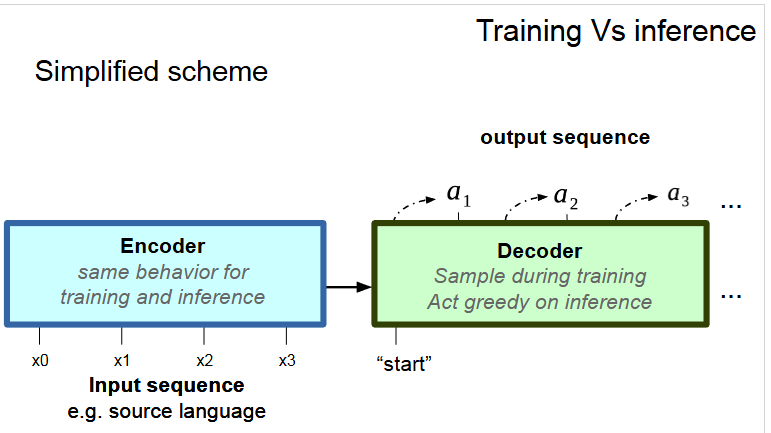
\includegraphics[width=0.85\textwidth]{figures/lecture11_training_vs_inference.png}
    \caption{В seq2seq encoder ведёт себя одинаково, а decoder при training может sample-ить, при inference действует greedy.}
\end{figure}

\subsection{Self-Critical Sequence Training}

\textbf{Self-Critical Sequence Training, SCST} --- метод, который использует inference mode как baseline.

Идея:

\begin{itemize}
    \item сгенерировать output в sampling mode;
    \item посчитать reward sampled output:
    \[
    R(s,a);
    \]

    \item сгенерировать output в greedy inference mode;
    \item посчитать reward greedy output:
    \[
    R(s,a_{inference}(s));
    \]

    \item использовать difference как advantage.
\end{itemize}

Advantage в SCST:

\[
A(s,a)
=
R(s,a)
-
R(s,a_{inference}(s)).
\]

Policy gradient:

\[
\nabla J
=
\mathbb{E}
[
\nabla \log \pi_\theta(a\mid s)
A(s,a)
].
\]

% Слайд 50. Self-critical sequence training: advantage = reward(sampled) - reward(greedy inference).
\begin{figure}[H]
    \centering
    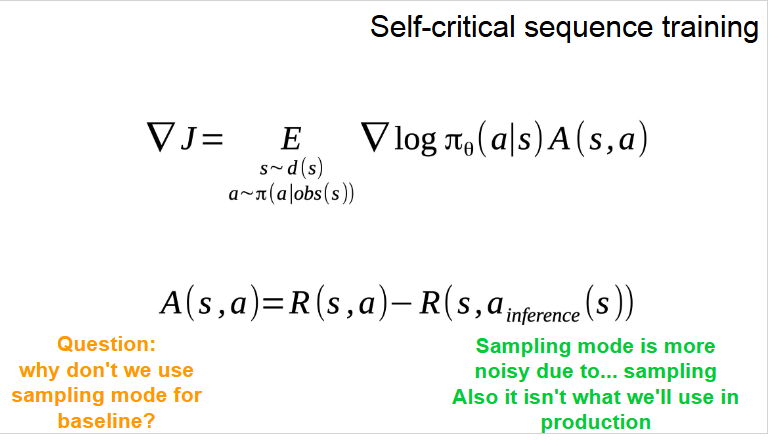
\includegraphics[width=0.85\textwidth]{figures/lecture11_scst_advantage.png}
    \caption{SCST использует greedy inference output как baseline для sampled output.}
\end{figure}

\subsection{Почему baseline берётся из inference mode}

Можно было бы использовать sampling mode для baseline, но это хуже по двум причинам:

\begin{itemize}
    \item sampling baseline более noisy, потому что сам зависит от случайного sampling;
    \item в production обычно используется greedy или beam decoding, а не random sampling.
\end{itemize}

SCST сравнивает sampled output с тем, что модель реально сделала бы на inference. Если sampled output лучше greedy output, его вероятность увеличивается. Если хуже --- уменьшается.

\subsection{Интуиция SCST}

Если:

\[
R(s,a) > R(s,a_{inference}(s)),
\]

то:

\[
A(s,a)>0.
\]

Значит sampled sequence лучше текущего greedy поведения модели. Нужно увеличить вероятность sampled actions.

Если:

\[
R(s,a) < R(s,a_{inference}(s)),
\]

то:

\[
A(s,a)<0.
\]

Значит sampled sequence хуже baseline. Нужно уменьшить её вероятность.

Таким образом, модель учится улучшать свою собственную inference-policy.

\subsection{Image Captioning with SCST}

В image captioning:

\begin{itemize}
    \item input \(x\) --- изображение;
    \item output \(y\) --- caption;
    \item reward --- метрика качества caption, например CIDEr;
    \item dataset --- MSCOCO.
\end{itemize}

Обучение:

\begin{enumerate}
    \item pre-training:
    \[
    \max_\theta \log P_\theta(\text{caption}\mid \text{image});
    \]

    \item fine-tuning:
    \[
    \max_\theta \mathbb{E}[CIDEr(\hat{y}, y_{ref})].
    \]
\end{enumerate}

SCST использует self-critical baseline для уменьшения дисперсии gradient.

\subsection{Результаты SCST}

В презентации приводится таблица результатов для image captioning. Модели сравниваются по нескольким метрикам:

\begin{itemize}
    \item CIDEr;
    \item BLEU4;
    \item ROUGEL;
    \item METEOR.
\end{itemize}

Важный вывод: когда SCST оптимизирует конкретную метрику, качество по этой метрике обычно растёт.

Например, оптимизация CIDEr даёт высокий CIDEr score, оптимизация BLEU улучшает BLEU, и так далее.

% Слайд 54. SCST results: модели, оптимизирующие конкретную метрику, улучшают соответствующий validation score.
\begin{figure}[H]
    \centering
    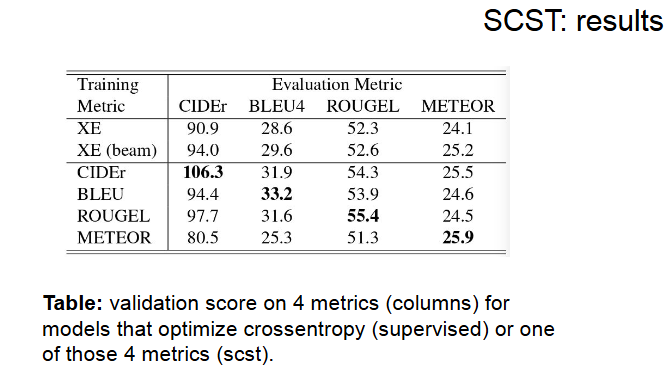
\includegraphics[width=0.85\textwidth]{figures/lecture11_scst_results.png}
    \caption{SCST позволяет напрямую оптимизировать целевые sequence-level метрики вроде CIDEr, BLEU, ROUGE и METEOR.}
\end{figure}

\subsection{Common pitfalls}

При RL fine-tuning sequence models важно учитывать несколько рисков.

\subsubsection{Reward hacking}

Агент может найти способ ``обмануть'' reward:

\[
\text{maximize metric} \neq \text{solve intended task}.
\]

Например, модель может выучить шаблон, который хорошо выглядит для автоматической метрики, но плохо соответствует реальному качеству.

\subsubsection{Overfitting}

Модель может overfit-иться под training data или под конкретную reward metric.

Поэтому нужно проверять validation performance и желательно использовать несколько метрик и human evaluation.

\subsubsection{Долгое обучение}

RL methods обычно дольше обучаются from scratch. Поэтому почти всегда полезно сначала pre-train model in supervised mode.

\subsection{Практические советы}

Для seq2seq RL fine-tuning полезны следующие приёмы:

\begin{itemize}
    \item pre-train model in supervised mode;
    \item использовать entropy regularization;
    \item использовать L2 regularization logits;
    \item применять better sampling techniques;
    \item использовать стандартные seq2seq tricks;
    \item для большого vocabulary использовать bottleneck или softmax improvements.
\end{itemize}

\subsection{Bonus: discrete GANs}

В обычном GAN есть:

\begin{itemize}
    \item generator \(G(z)\);
    \item discriminator \(D(x)\);
    \item real data;
    \item fake data.
\end{itemize}

Discriminator выдаёт вероятность, что объект real:

\[
D(x)=P(real\mid x).
\]

Для непрерывных данных gradient от discriminator может проходить в generator.

Но если generator выдаёт discrete objects, backpropagation через sampling невозможен.

Примеры discrete generation:

\begin{itemize}
    \item text;
    \item music notes;
    \item molecules;
    \item binary image masks.
\end{itemize}

В этом случае generator можно обучать через policy gradient: generator рассматривается как policy, discrete output --- как action, а reward приходит от discriminator.

Также возможны альтернативы:

\begin{itemize}
    \item Gumbel-Softmax;
    \item hard attention tricks;
    \item discrete loss functions;
    \item binary network tricks.
\end{itemize}

\subsection{Сравнение supervised seq2seq и RL fine-tuning}

\begin{table}[H]
\centering
\begin{tabular}{p{0.45\textwidth} p{0.45\textwidth}}
\toprule
\textbf{Supervised seq2seq} & \textbf{RL fine-tuning / Policy Gradient} \\
\midrule

Требует reference outputs. &
Требует reward function. \\

Оптимизирует likelihood:
\[
\log P(y\mid x).
\]
&
Оптимизирует expected reward:
\[
\mathbb{E}[R(x,\hat{y})].
\]
\\

Обучается на reference prefixes. &
Обучается на generated outputs. \\

Меньшая дисперсия gradient. &
Большая дисперсия gradient. \\

Есть distribution shift между training и inference. &
Distribution shift меньше, потому что модель учится на собственных outputs. \\

Хорошо для pre-training. &
Хорошо для post-training под конкретную метрику. \\

\bottomrule
\end{tabular}
\caption{Сравнение supervised seq2seq learning и RL fine-tuning.}
\end{table}

\subsection{Главные выводы}

\begin{itemize}
    \item Sequence generation можно рассматривать как RL-задачу.
    \item Decoder policy выбирает следующий токен:
    \[
    a_t \sim \pi_\theta(a_t\mid obs(s_t)).
    \]

    \item Reward может быть black-box sequence-level metric, например BLEU или CIDEr.
    \item Supervised seq2seq learning оптимизирует likelihood reference outputs.
    \item Supervised learning страдает от distribution shift: training использует reference prefix, inference использует generated prefix.
    \item В machine translation и диалогах часто существует много корректных outputs.
    \item Policy gradient обучается на собственных outputs и может напрямую оптимизировать целевую метрику.
    \item Policy gradient имеет cold start problem и высокую дисперсию.
    \item Поэтому используют:
    \[
    \text{supervised pre-training}
    \rightarrow
    \text{RL fine-tuning}.
    \]

    \item SCST использует greedy inference output как baseline:
    \[
    A(s,a)
    =
    R(s,a)-R(s,a_{inference}(s)).
    \]

    \item SCST хорошо подходит для image captioning и других seq2seq-задач с внешней метрикой.
    \item Policy gradient можно использовать для discrete generators, например text GANs.
\end{itemize}

\subsection{Что важно помнить к экзамену}

\begin{enumerate}
    \item Общий objective:
    \[
    J
    =
    \mathbb{E}_{s\sim d(s),\,a\sim\pi(a\mid obs(s))}
    [
    R(s,a)
    ].
    \]

    \item Supervised seq2seq:
    \[
    \max_\theta \log P_\theta(y\mid x)
    =
    \max_\theta
    \sum_t
    \log P_\theta(y_t\mid x,y_{<t}).
    \]

    \item Distribution shift:
    \[
    \text{training: } y_{0:t}\sim reference,
    \]
    \[
    \text{inference: } \hat{y}_{0:t}\sim model.
    \]

    \item Seq2seq as POMDP:
    \begin{itemize}
        \item state --- translation/conversation state;
        \item observation --- previous words;
        \item action --- next word;
        \item reward --- BLEU/CIDEr/domain metric.
    \end{itemize}

    \item Log-derivative trick:
    \[
    \nabla_\theta \pi_\theta(z)
    =
    \pi_\theta(z)
    \nabla_\theta \log \pi_\theta(z).
    \]

    \item Policy gradient:
    \[
    \nabla_\theta J
    =
    \mathbb{E}
    [
    \nabla_\theta
    \log \pi_\theta(a\mid s)
    R(s,a)
    ].
    \]

    \item Supervised gradient:
    \[
    \nabla \ell_{lh}
    =
    \mathbb{E}_{s,a_{opt}\sim D}
    [
    \nabla \log \pi_\theta(a_{opt}\mid s)
    ].
    \]

    \item Policy gradient обучается на:
    \[
    a\sim\pi_\theta(a\mid obs(s)).
    \]

    \item Supervised learning требует хорошие reference \(y_{opt}\), RL требует reward function.

    \item SCST advantage:
    \[
    A(s,a)
    =
    R(s,a)
    -
    R(s,a_{inference}(s)).
    \]

    \item SCST gradient:
    \[
    \nabla J
    =
    \mathbb{E}
    [
    \nabla \log \pi_\theta(a\mid s)
    A(s,a)
    ].
    \]

    \item Практическая схема:
    \[
    \text{pre-train with cross-entropy}
    \rightarrow
    \text{fine-tune with RL / SCST}.
    \]

    \item В discrete GANs generator можно обучать policy gradient, потому что backpropagation через discrete sampling невозможен.
\end{enumerate}
```





% =====================================

\end{document}